% !TEX root = ../These_Robin_Master.tex
\chapter{Évaluer et paramétrer un modèle de simulation complexe en situation d'inter-disciplinarité}
\label{chap:chap3}
\begin{center}
{\large Version \hl{2019-11-24}}
\end{center}

\begin{itemize}
	\item 31/10/2019 : Fusion anciens chapitre 3 (évaluation) et 4 (paramétrage)
	\item 08/11/2019 : Fin reprise + Impression Lena
	\item 11/11/2019 : Reprises commentaires Lena du 24/11/2017 + finalisation
	\item 19/11/2019 : Dernier round reprises Lena
	\item 24/11/2019 : Fin reprise + envoi relecture :
		\begin{itemize}
			\item Seb : Intro + 3.1 + 3.2.1 et 3.2.2 (pas la 3.2.3) + Conclusion
			\item Clem : Intro + Partie 3.3 + Conclusion
			\item Paul G. : 3.2.3
			\item => \hl{Retour si possible le jeudi 05/12/2019}
		\end{itemize}
\end{itemize}
\setcounter{minitocdepth}{2}
\minitoc
\clearpage

\phantomsection
\section*{Introduction}
\label{sec:chap3-4-intro}
\addcontentsline{toc}{section}{Introduction}

Dans le chapitre précédent, nous avons présenté un modèle, SimFeodal, dont l'objectif est de répondre à un questionnement thématique (\hl{ref 2.1.2}) portant les phénomènes de polarisation, de hiérarchisation et de fixation de l'habitat paysan entre les IX$^e$ et XIII$^e$ siècles.
Pour juger de la capacité du modèle à reproduire ces processus empiriques, on on procède à une \og évaluation\fg{} du modèle.
Ce type d'évaluation prend appui sur un ensemble de critères : plus ceux-ci sont remplis, meilleure sera l'évaluation, et plus le modèle sera jugé satisfaisant.

L'évaluation de modèle est un domaine incontournable et fortement étudié dans le champ de la modélisation, quel que soit le type de modèles sur cette évaluation porte.
Dans le cas de SimFeodal, modèle descriptif et complexe, l'évaluation ne peut se faire de manière formelle, c'est-à-dire analytique, tant les interactions entre agents et mécanismes sont nombreuses, non linéaires, et donc non prédictibles.
L'évaluation ne peut donc être qu'expérimentale, en analysant le comportement du modèle sur la base de ses sorties.

SimFeodal pose de plus le problème d'être un modèle basé sur des connaissances expertes plutôt que sur des données directement intégrables ou confrontables.
Cela en complexifie l'évaluation, car les approches classiques sont peu adaptées à ce type de modélisation interdisciplinaire guidé par la théorie et où les données empiriques sont lacunaires.
Il est en effet difficile de quantifier le comportement attendu du modèle.

Les difficultés liées à l'évaluation du modèle sont renforcées par le type de construction mis en place pour SimFeodal, qui est un modèle exploratoire dans lequel l'évaluation n'a pas vocation à valider une version définitive et statique du modèle, mais au contraire à guider son amélioration par des ajustements successifs.

Dans le chapitre précédent, on décrivait par exemple une \og version\fg{} du modèle, intitulée \og version 6.3\fg{}, ce qui montre qu'auparavant, il y a nécessairement eu au moins 5 versions préalables, et sans doute bien plus de sous-versions.
Ce chapitre vise à présenter le processus d'amélioration du modèle que nous nommons \og paramétrage\fg{}, c'est-à-dire l'approche théorique et empirique qui a guidé l'évolution de SimFeodal, à partir des retours réguliers de l'évaluation du modèle.

Dans ce chapitre, nous présenterons en premier lieu la démarche globale d'évaluation, et en particulier une proposition de méthode fondée sur l'évaluation visuelle -- adaptée aux modèles du type de SimFeodal.
Nous spécifierons cette approche en l'appliquant au cas de SimFeodal, c'est-à-dire en présentant les critères retenus pour l'évaluation du modèle.
Nous décrirons ensuite le paramétrage du modèle, son articulation avec l'évaluation, et nous mènerons une analyse rétrospective de l'évolution de SimFeodal.

\section{Comment évaluer un modèle ?}\label{sec:evaluer-modele}

Depuis les travaux précurseurs en simulation informatique \autocite{naylor_verification_1967,hermann_validation_1967,sargent_validation_1979} jusqu'aux recherches contemporaines \autocite{amblard_evaluation_2006,banos_pour_2013,augusiak_merging_2014, rey-coyrehourcq_plateforme_2015}, la plupart des chercheurs ont toujours mis en avant qu'un modèle de simulation non évalué n'avait ni utilité -- pour \cite{naylor_verification_1967} notamment --, ni validité.
Sans caricaturer ces écrits, on peut noter que tous cantonnent les modèles non évalués à des \og jeux\fg{} ou encore, pour les plus modérés, à des outils uniquement pédagogiques.

Comme indiqué dans le \hl{chapitre 1}, nous considérons SimFeodal comme un modèle résolument exploratoire, en particulier par la dimension heuristique qui le caractérise : les résultats produits par le modèle n'ont pas vocation à être mobilisés directement, ce sont des supports à la synthèse et à la ré-organisation de connaissances expertes sur le cas d'étude analysé.
On pourrait dès lors se passer d'en mener une évaluation quelconque.

Il nous semble pour autant que l'exercice intellectuel que constitue la (co-)construction d'un modèle de simulation perdrait de son intérêt intrinsèque s'il ne donnait lieu à des procédures, quelles qu'elles soient, ayant pour objectif d'assurer une certaine qualité au modèle, à défaut de lui garantir une validation stricte.

Nous sommes en effet convaincus que même pour des modèles visant à \og assister la construction de théories\fg{}
\footnote{
	\og Simulation models to support theory building -- so-called heuristic modelling -- \textelp{}.\fg{}
} pour reprendre les termes de \textcite[260]{lake_trends_2014}, ou encore, selon la classification alternative de l'auteur, pour les modèles à utilité \og de développement\fg{}
\footnote{
	\og 'developmental' utility\fg{}, c'est-à-dire les modèles dont le développement et l'implémentation bénéficient aux chercheurs qui y prennent part plutôt qu'à ceux qui se contentent de les utiliser a posteriori.
}, les différents outils d'évaluation permettent d'acquérir une connaissance précieuse sur l'objet modélisé, ne serait-ce que par les effets collatéraux qu'entraîne l'évaluation d'un modèle.
Qu'un modèle soit statistique ou à base d'agents, de type descriptif ou explicatif, à visée pédagogique ou prédictive, ou encore constitue un modèle \og hybride\fg{} entre ces catégories, un modèle de simulation demeure un modèle qu'il convient d'évaluer pour être en mesure d'en tirer des connaissances \autocite[299-300]{sargent_history_2017}.

Sans entrer dans les spécificités conceptuelles de ce qu'est l'évaluation d'un modèle ou de l'histoire de ces méthodes
\footnote{
	En particulier parce que ce sujet a été très largement traité dans un travail de thèse récent au sein de notre laboratoire de recherche \autocite[pp. 58--184]{rey-coyrehourcq_plateforme_2015}, travail auquel nous renvoyons vivement pour plus d'approfondissements.
}, nous nous contenterons dans la suite de cette partie de donner une vision aussi succincte que possible de ce qu'est l'évaluation, en particulier pour en dégager les méthodes employées usuellement.
Cela nous permettra en particulier de défendre et de promouvoir l'une de ces méthode, la validation visuelle, que nous jugeons très adaptée dans le cadre de co-constructions interdisciplinaires de modèles.

\subsection{Évaluation, validation, vérification\ldots}

Il nous semble important de commencer cette partie par un point de définition et de clarification des concepts mobilisés, non pas par convention, mais parce que les usages en matière d'emploi des termes d'évaluation, de validation (méthodologique, formelle\ldots) ou encore de vérification sont particulièrement diffus et trompeurs dans la littérature relative à la modélisation, y compris dans le champ plus restreint de la simulation à base d'agents en sciences humaines et sociales.

Depuis les travaux fondateurs, dans les années 1960, la logique qui consiste à éprouver un modèle -- c'est-à-dire à vérifier qu'il corresponde correctement d'une part (1) au système qu'il décrit, et d'autre part à
(2) la manière dont il est décrit -- donne lieu à différentes terminologies.
On notera en particulier que les deux articles considérés comme pionniers, tous deux parus en 1967, reposent pour l'un sur la notion de vérification (\textit{verification}) \autocite{naylor_verification_1967}, et pour l'autre sur celle de validation \autocite{hermann_validation_1967}, sans pour autant que la distinction entre les deux approches puisse être vue comme consistante.
Quelques décennies plus tard, une fois la pratique de simulation informatique plus développée et mûre, un consensus de pratique a été adopté autour de l'expression englobante de \og Validation, Verification and Testing techniques (VV\&T)\fg{}, par l'entremise d'une proposition de \textcite{balci_validation_1994} de clarification et de définition de chacun de ces composants.
Pour reprendre ses mots en une distinction devenue courante en simulation à base d'agent, la \textit{validation} consiste à concevoir le bon modèle 
\footnote{
	\og Model validation deals with building the \textit{right} model.\fg{} \autocite[121]{balci_validation_1994}
} -- sens (1) exposé plus haut --,
alors que la \textit{verification} permet de s'assurer que le modèle est bien construit
\footnote{
	\og Model verification deals with building the model \textit{right}.\fg{} \autocite[123]{balci_validation_1994}
} -- sens (2).
Le \og \textit{Testing}\fg{} correspond aux techniques mises en œuvre, et s'applique donc indistinctement à ces deux termes (\textit{validation} et \textit{verification}).

En dépit de cette définition stricte, les usages persistent dans une absence de distinction formelle entre vérification et validation, le plus souvent en englobant ces pratiques dans le terme plus large et moins défini d'\og évaluation\fg{}.
Il n'est d'ailleurs pas rare que ces trois termes soient employés de manière interchangeable, voir intervertie, comme un recensement rigoureux des usages le démontre \autocite{augusiak_merging_2014}.
Dans cet article, les auteurs mènent une méta-analyse de la littérature sur les usages de chacun des termes liés à l'évaluation\footnote{
	\textit{Corroboration}, \textit{Evaluation}, \textit{Testing}, \textit{Validation}, \textit{Verification} et \textit{Substantiation}
}, et en particulier de celui de \textit{validation}, et du sens signifié par leurs auteurs respectifs.
Ils en tirent le constat qu'une large partie des termes analysés a été employé par plusieurs auteurs leur affectant des sens contradictoires.
Par exemple : \og the term ``validation'' has been given virtually any possible meaning in this context\fg{} \autocite[120]{augusiak_merging_2014}.

\paragraph*{}
Les auteurs de cette étude puisent dans ce constat les besoins d'une nouvelle terminologie, unique et explicite, permettant de dépasser notamment les successions d'attrait et de rejet que la notion de validation entraîne de par son positivisme.
Ils proposent ainsi un nouveau terme, l'\og \textit{evaludation} \fg{}, assorti à une typologie de concepts -- explicitement définis  \autocite[table 2, p. 125]{augusiak_merging_2014} -- liés à l'évaluation permettant d'identifier l'objet et le sujet de chacune des phases du cycle d'\og évaludation\fg{} (voir \cref{fig:schema_evaludationl}).

\begin{figure}[H]
	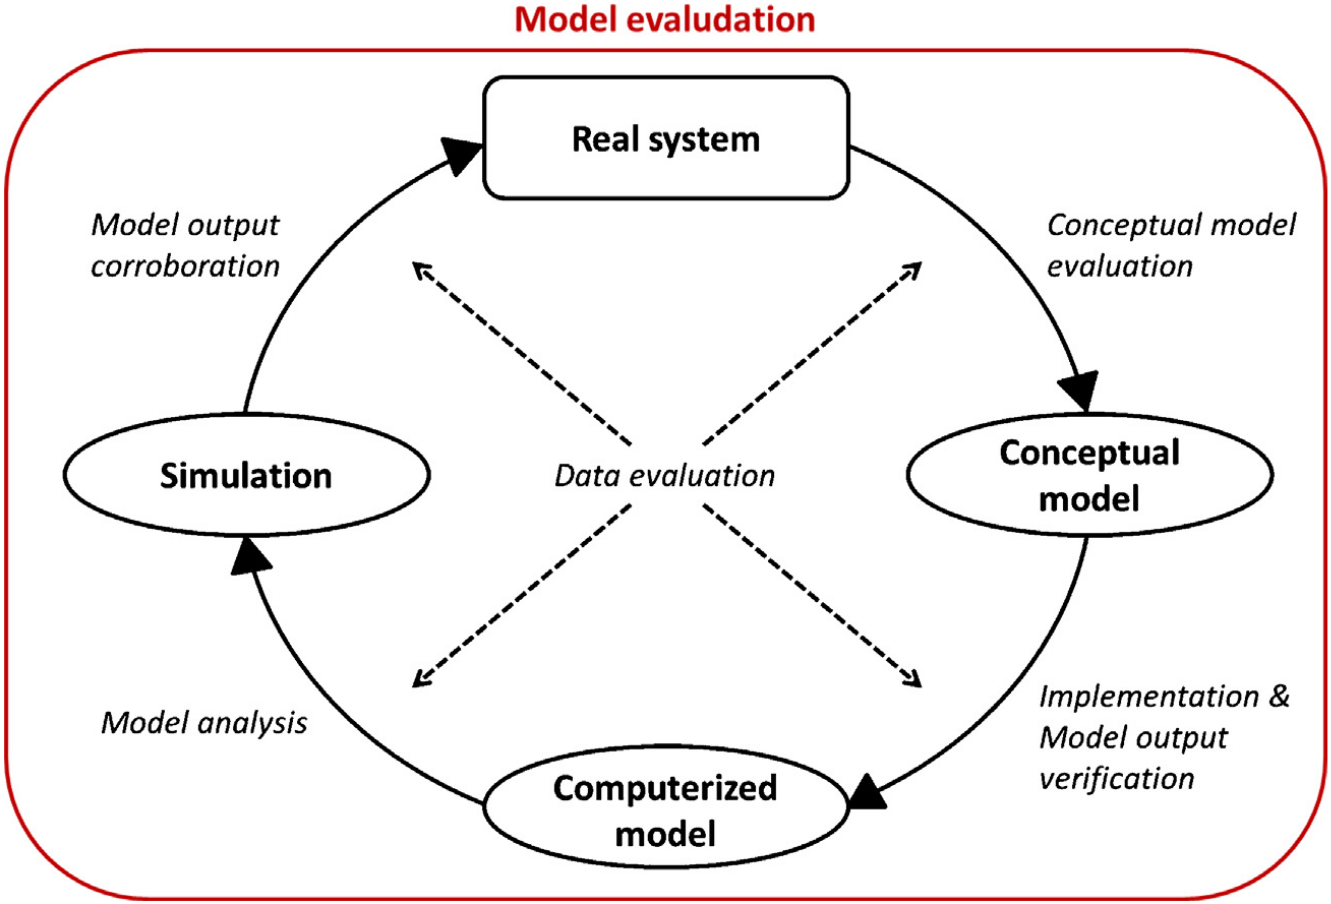
\includegraphics[width=\linewidth]{img/Schema_Augusiak_evaludation.png}
	\caption[Représentation schématique du cycle de modélisation et de la typologie des termes relatifs à l'évaluation de modèle.]{Représentation schématique du cycle de modélisation et de la typologie des termes relatifs à l'évaluation de modèle, dans \textcite[Fig. 1, p. 121]{augusiak_merging_2014}}
	\label{fig:schema_evaludationl}
\end{figure}

Dans ce schéma, il est intéressant de noter que le terme de \og validation\fg{} n'est nul part employé (si ne n'est dans le mot-valise \textit{evaludation}), au contraire de celui d'\og \textit{evaluation}\fg{} assez omniprésent.
Les auteurs se détachent de l'usage de \og \textit{validation}\fg{} en raison de la connotation très positiviste et \og binaire\fg{} de ce mot : elle peut impliquer qu'un modèle est soit valide, soit invalide, loin du gradient qu'accepte l'évaluation.
Notons que l'item central du schéma, l'évaluation des données (\textit{data evaluation}) qui intervient pour l'évaluation de chacun des types de modèle, a une signification plus ouverte qu'on ne pourrait l'entendre au sens premier.
\textcite[121]{augusiak_merging_2014} y incluent ainsi des connaissances extraites des données en tant que telles : \og The term ``data'' also refers
to patterns \autocite{grimm_pattern-oriented_2012} or, in economists' termi-
nology, ``stylised facts'', which are general trends and signals in data,
observations, and empirical knowledge.\fg{}

Nous partageons absolument le besoin formel, identifié par les auteurs de cette étude, de définir un nouveau terme dans leur proposition, et nous souscrivons à leur approche de définition.
Il nous semble toutefois, et nous le déplorons, que ce travail n'ait pas encore suffisamment percolé dans la communauté scientifique, et en particulier dans le monde francophone.
Au moment de rédiger ces lignes, très peu d'auteurs en font un usage en français, et surtout sous la forme de recension plus que d'utilisation du concept \autocite[par exemple][89,436]{rey-coyrehourcq_plateforme_2015}.

Par soucis d'homogénéité et de compréhension par un plus grand nombre de ce travail, nous nous contenterons donc de nous inscrire dans les choix de \textcite[voir \cref{enc:lexique-eval-amblard}]{amblard_evaluation_2006}, en particulier parce qu'ils nous semblent assez largement adoptés dans la communauté scientifique francophone de modélisation en sciences humaines et sociales, quand bien même ces concepts nous paraissent moins robustes que ceux présentés auparavant.

\clearpage
\begin{encadre}{Évaluation, validation interne et externe}{lexique-eval-amblard}
\renewcommand{\thempfootnote}{\alph{mpfootnote}}

Pour \textcite{amblard_evaluation_2006}, on emploie le concept d'\textbf{évaluation} pour définir l'approche d'ensemble, et on distingue alors \og \textbf{validation interne}\fg{} -- correspondant à la \textit{verification} définie par \textcite{balci_validation_1994}, c'est-à-dire s'assurer de la bonne conception du modèle, et \og \textbf{validation externe}\fg{} -- ce que \citeauthor{balci_validation_1994} nomme \textit{validation}, soit l'assurance que le modèle est adapté à ce qu'il cherche à représenter.

\begin{quotation}
\noindent \og Il est classique de différencier deux étapes dans la validation : interne et externe.
\begin{itemize}
	\item La phase de vérification ou \textbf{validation interne} comprend d'abord une vérification de conformité entre les spécifications et le programme implémenté et pose la question : est-ce que le modèle implémenté est bien celui que je voulais implémenter ? [...]
	Ensuite, la validation interne concerne la recherche et l'identification des propriétés du modèle.
	Dans le cas des simulations multi-agents, des preuves logiques ne peuvent être obtenues et se pose alors la question : est-ce que mon modèle possède les propriétés attendues ?
	Parmi ces bonnes propriétés, on considère par exemple la robustesse ou des études de sensibilité pour vérifier si les réponses sont bien différenciées sur l'espace des paramètres.
	Cette phase de validation interne concerne de fait une validation dans le contexte ou la logique propre du modèle.

	\item La deuxième phase de validation, la \textbf{validation externe}, correspond à l'évaluation de l'adéquation entre le modèle et le phénomène réel dont il est censé rendre compte.
	Pour cette dernière phase, la comparaison aux données empiriques ou le fait que le modèle soit capable d'exhiber des faits stylisés identifiés sur le système modélisé sont des critères clés.
\end{itemize}
Ainsi, ce qui est étudié au travers des simulations, ce sont tout d'abord les propriétés systémiques (structurelles et dynamiques) du modèle, les formes qui peuvent apparaître du fait des hypothèses posées (validation interne) ;
ensuite est évaluée la pertinence du modèle vis-à-vis de situations que l'on souhaite représenter ou prévoir (validation externe).\fg{}\\
	\mbox{}~ \hfill \cite[110-111]{amblard_evaluation_2006}
\end{quotation}
\end{encadre}

\clearpage

\subsection{Les étapes de l'évaluation d'un modèle}

Parmi les nombreuses techniques disponibles pour l'évaluation, il est courant de privilégier telle ou telle méthode en fonction de la phase d'avancement d'un modèle.
Traditionnellement, l'usage veut ainsi que le modélisateur tende vers des méthodes de plus en plus formelles à mesure que l'évaluation progresse\footnote{
	Voir par exemple la typologie des méthodes d'évaluation, des plus \og informelles \fg{} aux méthodes \og formelles \fg{} chez \textcite[figure 3, p. 131]{balci_validation_1994}}.
Les schémas des étapes d'évaluation de \citeauthor{klugl_validation_2008} (\cref{fig:schema_kluegl}) et de \citeauthor{ngo_calibration_2012} (\cref{{fig:schema_ngo}}) constituent un bon résumé de cette progression -- représentée de manière itérative quand bien même chaque auteur insiste sur le fait que ces étapes doivent être menées en multipliant les allers-retours entre elles -- que l'on peut brièvement décrire plus avant.

\begin{figure}[H]
	\center
	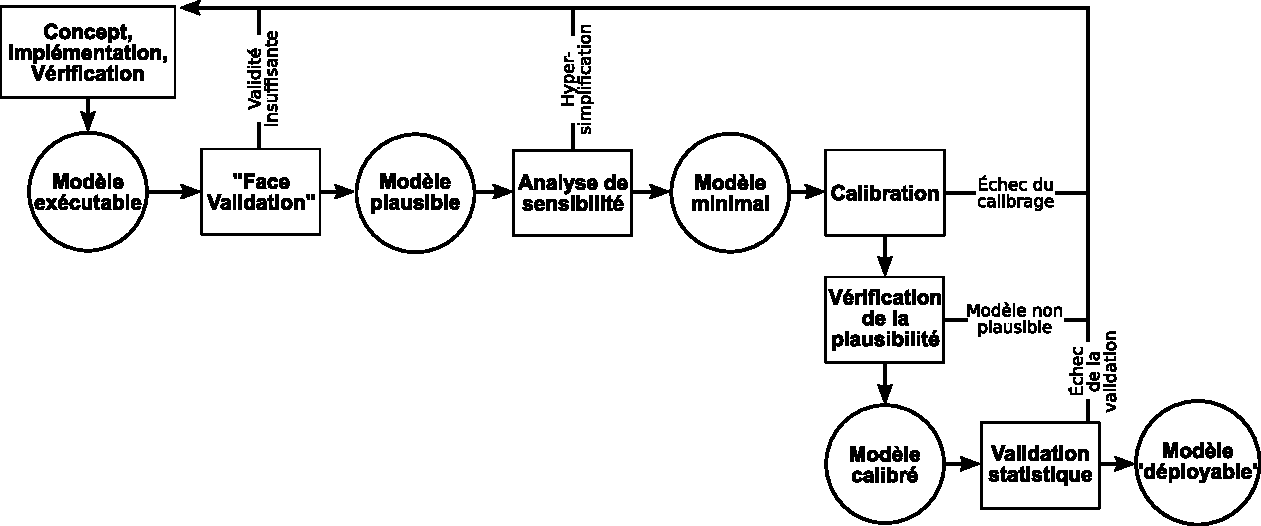
\includegraphics[width=\linewidth]{img/schema_kluegl_traduit.pdf}
	\caption[Une esquisse de procédure générale de validation de modèles de simulation à base d'agents.]{Une esquisse de procédure générale de validation de modèles de simulation à base d'agents, traduit d'après \textcite[fig. 1 p. 42]{klugl_validation_2008}}
	\label{fig:schema_kluegl}
\end{figure}
\bigskip
\begin{figure}[H]
	\center
	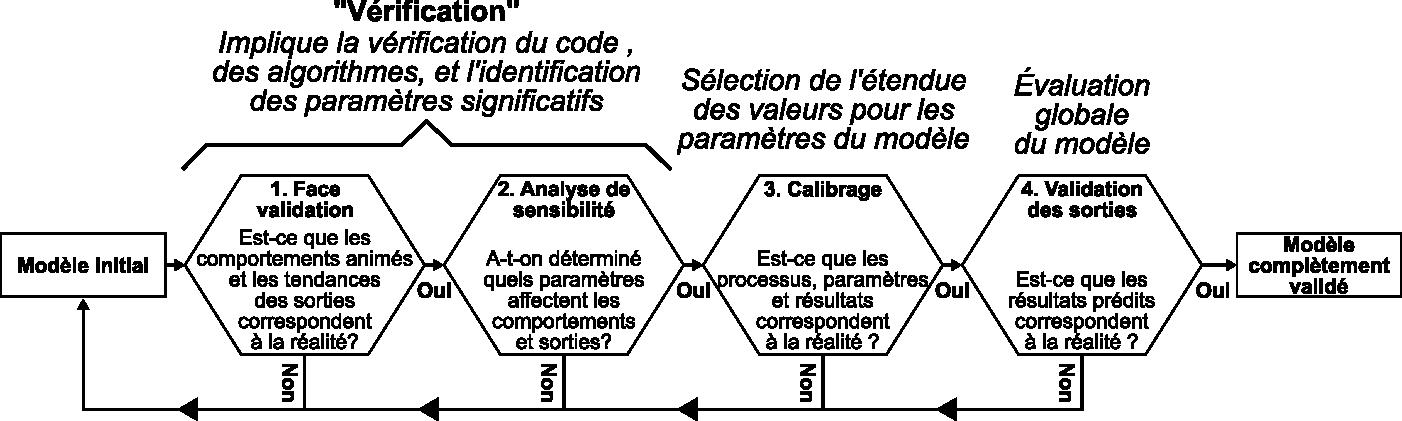
\includegraphics[width=\linewidth]{img/schema_ngo.pdf}
	\caption[Procédure générale de validation d'un modèle à base d'agents.]{Une procédure générale de validation d'un modèle à base d'agents, traduit d'après \textcite[fig. 10.1 p. 183]{ngo_calibration_2012}}
	\label{fig:schema_ngo}
\end{figure}


\paragraph{\og \textit{Face validation}\fg{}.}
La première étape, de \og \textit{face validation}\fg{}, consiste ainsi à vérifier visuellement, en se confortant à des intuitions sur le comportement attendu, la plausibilité du modèle.
On entend par plausibilité la potentielle adéquation entre le déroulement (en termes de dynamiques observés) et l'issu (au travers des données produites) d'une simulation, et les connaissances expertes que l'on possède sur le système modélisé.
Cette étape est souvent considérée comme une mesure préalable relevant du bon sens plus que de l'évaluation strictement dite, et relève autant de la validation interne que de la validation externe.
Nous reviendrons plus longuement dans les pages suivantes (voir \cref{subsec:face-validity}) sur cette étape essentielle d'après l'avis partagé dans la littérature mais néanmoins largement sous-exploité et méjugée à notre avis.

\paragraph{Analyse de sensibilité.}
Quand une première version du modèle a été implémentée, il est recommandé de procéder à l'analyse de sa \og sensibilité \fg{}, entendue à l'égard des paramètres du modèle : en faisant varier, selon des méthodes plus ou moins complexes
\footnote{
	Un point plus précis y est consacré dans le \hl{chapitre 6}
}, les valeurs des différents paramètres du modèle, on peut observer l'influence de chaque paramètre sur le déroulement du modèle.
Cette procédure, relative à la validation interne, intervient tôt, et doit être répétée lors de chaque modification majeure dans les mécanismes du modèle.
L'analyse de sensibilité permet en effet de simplifier le modèle conceptuel et son pendant implémenté :
	si l'analyse révèle qu'un paramètre, quelles que soient les valeurs qui lui sont attribuées, n'a qu'un effet minime voir négligeable sur les sorties du modèles, alors il peut être judicieux de supprimer ce paramètre ou le mécanisme qui le mobilise.
Réduire le nombre de paramètres ou de mécanismes d'un modèle peut sensiblement l'améliorer, selon le principe de parcimonie qui voudrait qu'un modèle plus simple soit meilleur\footnote{
	Les avis divergent nettement sur ce point, voir par exemple la définition de la \textit{simplicité} dans \textcite[120]{amblard_evaluation_2006}
}.
Même sans aller jusqu'à ce type de découvertes sur l'inutilité de certains paramètres, l'analyse de sensibilité permet de gagner en connaissance sur le fonctionnement d'un modèle complexe et/ou non-déterministe, ne serait-ce que parce qu'elle aide souvent le modélisateur à trouver une \og polarité \fg{} à l'effet des paramètres :
	si tel indicateur de sortie (voir \cref{subsec:indices-indicateurs}) croît quand on diminue les valeurs d'un paramètre et décroît quand on les augmente, alors on peut prévoir l'effet d'une modification de ce paramètre, ce qui peut éclairer le fonctionnement thématique du modèle.

\paragraph{Calibrage.}
Une fois le modèle mieux connu et surtout réduit à ses composantes nécessaires et suffisantes, on cherche à en améliorer la qualité de représentation, c'est-à-dire à faire en sorte, en jouant sur les valeurs de paramètres, que le modèle reproduise plus précisément le système qu'il décrit (validation externe) et qui correspond à l'observation empirique ou aux connaissances thématiques.
Cette démarche, nommée calibrage, soulève l'enjeu d'isoler, pour chaque paramètre, une étendue de valeurs acceptables et optimales.
La complexité -- au sens figuré -- de cette étape réside dans la complexité -- au sens propre -- du modèle qu'il convient de calibrer :
	dans un modèle complexe, où chaque mécanisme peut influencer chacun des autres mécanismes de manière non linéaire, la modification des valeurs d'un paramètre doit certes modifier l'état du modèle en lui-même, mais a le plus souvent tendance à modifier par là même l'optimalité des valeurs des autres paramètres.
Le problème ressemble à celui des vases communicants :
	pour que le modèle soit calibré, il faut que chaque valeur de paramètre soit optimale, mais la modification de chacun des paramètres peut dérégler l'effet des autres paramètres, et par la même les valeurs qu'ils doivent se voir attribuer.
On ne peut donc procéder paramètre par paramètre, en les réglant un par un, au risque d'entrer dans une boucle infinie de calibrage, mais au contraire, il est nécessaire de considérer l'ensemble -- ou un sous-ensemble -- des paramètres et de tester des valeurs qui iraient vers une optimisation du comportement du modèle.
Le calibrage en lui-même n'est pas à proprement parler une véritable procédure d'évaluation d'un modèle :
	il vise ainsi plutôt à \og améliorer\fg{} le modèle plus qu'à juger de sa validité.
Il s'agit ainsi plutôt d'une méthode et d'un problème d'optimisation que d'évaluation.
Les différents auteurs mettent toutefois en avant son intérêt dans l'évaluation de modèle en ce qu'il permet de garantir une meilleure validation externe du modèle puisqu'il aboutit à l'isolation d'étendues optimales de valeurs de paramètres :
	en menant de nouveaux tests d'évaluation (analyse de sensibilité, \textit{face validation}, etc.) \autocite[43]{klugl_validation_2008} sur les valeurs optimales identifiées, on peut évaluer si elles sont porteuses de sens d'un point de vue empirique ou au moins vis-à-vis de la connaissance experte du système modélisé.

\paragraph{Validation statistique.}
La validation statistique (\og \textit{output validation}\fg{} dans la \cref{fig:schema_ngo}) est sans doute la méthode d'évaluation la plus évidente pour quiconque a été amené à concevoir un modèle.
Il s'agit de confronter les données produites par le modèle -- les \textit{outputs} --
aux données empiriques -- ou observées -- qu'ils cherchent à reproduire.
Autrement dit, en termes statistiques, à s'assurer de la qualité de l'ajustement -- la \textit{goodness of fit} -- des données simulées.
On en mesure l'écart avec les données observées, quand de telles données sont disponibles, en cherchant à minimiser cet écart :
	plus l'écart est faible, alors plus le modèle parvient à reproduire les observations qui ont servi de support à sa conception et construction.
La validation statistique est donc une méthode de validation externe.
Les différents auteurs du champ de l'évaluation recommandent de ne mener cette étape qu'à la fin du processus d'évaluation, quand le réflexe en pratique est souvent de s'appuyer sur les données empiriques dès le début de la conception du modèle.
A défaut de suivre cette recommandation, le modélisateur risque d'emmener le modèle vers du \og sur-ajustement \fg{} (\textit{overfitting}), et d'inscrire alors celui-ci dans une forme de tautologie, le modèle étant alors construit précisément pour produire ce qu'il devrait plutôt faire émerger.
En conservant la validation statistique comme l'une des dernières étapes du cycle d'évaluation, c'est-à-dire en s'empêchant d'essayer de faire coller le modèle aux données qu'il doit reproduire, on s'assure de l'indépendance des mesures de l'ajustement, et on peut donc garantir une certaine objectivité quant à l'évaluation du modèle.

\paragraph{Validations formelles.}
Absentes des deux figures (\ref{fig:schema_kluegl} et \ref{fig:schema_ngo}), les méthodes de validation formelles sont toutefois porteuses d'un intérêt assez prégnant quand elles sont applicables.
Ces méthodes visent à résoudre de manière analytique un modèle complexe, c'est-à-dire à mettre en équations les comportements du modèle, leurs effets d'interaction, et à résoudre ces équations pour en proposer les ensembles finis de solutions ou d'états.
Cela requiert d'être en mesure de convertir un modèle exprimé dans un formalisme quelconque en un système d'équations dynamiques, et de parvenir en outre à résoudre l'ensemble de ce système.
Dans l'évaluation de modèles au sens large, cette étape peut se révéler indispensable et assez directe, par exemple quand il apparaît nécessaire d'évaluer un modèle basé sur la théorie des jeux, que l'on traite alors sous forme d'analyse de graphes.

Dans le cas plus spécifique des modèles à base d'agent, cas dans lequel nous nous inscrivons ici, la situation est plus difficile.
On emploie généralement la modélisation à base d'agents parce qu'elle encourage une approche anthropomorphique, plus aisément compréhensible et requérant moins de connaissances mathématiques que d'autres approches, mais aussi car il est terriblement complexe d'exprimer des systèmes dotés de multiples interactions, qui plus est multi-scalaires, sous forme de réseaux d'équations.
En un sens, on pourrait presque considérer qu'on fait appel à de la modélisation à base d'agents quand on ne peut mobiliser des modèles formels.
Le processus qui tendrait à formaliser, mathématiquement, des modèles agents est alors intrinsèquement contre-intuitif et difficile, quand bien même certains pensent que ce n'est pas une fatalité mais une question de temps\footnote{
	Par exemple Alain \textsc{Franc}, mathématicien dans le projet TransMonDyn :
	\og L'une des difficultés de l'acceptation des SMA comme modèles est que ces comportements sont très mal compris mathématiquement.
	Il existe peu de résultats qui permettent de relier un type de règles avec un type de comportement, alors que de tels liens sont à la base du succès des systèmes dynamiques, où l'on connaît (parfois\ldots) les gammes de paramètres qui mènent à un comportement d'équilibre, cyclique ou chaotique, et l'on sait qu'il ne peut y en avoir d'autres.
	[...]
	Il existe donc une tension entre, d'un côté, les systèmes dynamiques qui forment une théorie riche et solide de modélisation mathématique, mais pour un nombre assez restreint de situations (bien des difficultés apparaissent dans le cadre non linéaire, que l'on peut lire dans la richesse des travaux sur la modélisation de la turbulence par exemple) et, d'un autre côté, les SMA qui permettent des simulations à partir de règles plus riches et diversifiées, mais pour des résultats dont la compréhension mathématique très souvent nous échappe (il y a peu de théorèmes).
	On peut donc dire en résumé que les SMA sont « en avance » sur la compréhension mathématique des systèmes dynamiques et peuvent proposer des cas d'études aux mathématiciens.\fg{}
	\autocite[Annexe 2, \og Retour sur les SMA comme outil et cadre conceptuel de modélisation.\fg{}, pp. 479-482 ]{ouriachi_lelaboration_2018}
}.

Si la nature même de cet exercice implique vraisemblablement que peu s'y essayent, on notera tout de même que quelques auteurs \autocite{zhang_tipping_2011,grauwin_dynamic_2012}\footnote{
	\hl{Lena : regarder Axelrod et Axtell, dans leur article sur les 4 modes d'utilisation d'un SMA, article très maths. --> \textbf{Je ne trouve pas cette référence}.}
} sont parvenus à résoudre de manière analytique un modèle foncièrement pensé comme un modèle agent -- en automate cellulaire en l'occurrence --, le modèle de Schelling (voir \cref{enc:param-schelling}).
En dehors de l'intérêt que cela peut représenter pour la connaissance de ce modèle en particulier, rappelons tout de même que le modèle de Schelling a été énoncé à la fin des années 1960, que c'est un modèle particulièrement parcimonieux, et qu'il a tout de même fallu attendre le tournant des années 2010 afin d'y trouver une solution formelle.
Notons enfin que pour certains auteurs, dont l'un des pères de la modélisation à base d'agents informatiques \textcite{epstein2006remarks}, la résolution analytique de modèles de simulation à base d'agents n'est pas véritablement un enjeu, l'objectif étant d'utiliser le paradigme le plus \og éclairant\fg{} pour un problème donné :
\begin{quotation}
	\noindent \og
	The oft-claimed distinction between computational agent models, and equation-based models is illusory.
	Every agent model is, after all, a computer program (typically coded in a structured or object-oriented programming language).
	As such, each is clearly Turing computable (computable by a Turing machine).
	But, for every Turing machine, there is a unique corresponding and equivalent partial recursive function [see Hodel (1995)].\\
	\textelp{}\\
	So, in principle, one could cast any agent-based computational model as an explicit set of mathematical formulas (recursive functions).
	In practice, these formulas might be extremely complex and difficult to interpret.
	But, speaking technically, they surely exist.\textelp{}
	In any case, the issue is not whether equivalent equations exist, but which representation (equations or programs) is most illuminating.
	\fg{}\\
	\mbox{}~ \hfill \textcite[1590-1591]{epstein2006remarks}
\end{quotation}

Notons tout de même une dernière piste, intermédiaire, qui permet d'approcher de l'analyse formelle de modèles à base d'agents.
Un collectif de chercheurs a conçu un modèle descriptif et complexe de la participation électorale en partant des comportements individuels des électeurs \autocite[\og{}Modèle 1\fg{}]{edmonds2014complex,fieldhouse_cascade_2016}.
En accord avec les principes de la modélisation KIDS \autocite{edmonds_kiss_2005}, proposé par l'un des membres de ce collectif, les chercheurs ont ensuite procédé à une large simplification du modèle, notamment en réduisant une partie de ses aspects les plus spécifiques (réseaux sociaux des électeurs et différenciation des partis politiques entre autre) \autocite[\og{}Modèle 2\fg{}]{lafuerza_2_staged_2016}.
En repartant de cette version parcimonieuse du modèle, les chercheurs ont alors re-construit une nouvelle version du modèle, encore plus parcimonieuse et analysable de manière formelle \autocite[\og{}Modèle 3\fg{}]{lafuerza_3_simplification_2016}.
Après avoir démontré les liens entre le modèle 1 et le modèle 2, puis entre le modèle 2 et le modèle 3, les auteurs ont pu montrer à l'aide de l'évaluation formelle du modèle 3 que certains mécanismes du modèle 1, empiriquement pensés importants, n'avaient en fait qu'un effet très modéré.
\textcite{lafuerza_3_simplification_2016} s'appuient sur cette expérience pour démontrer l'utilité de la méthode KIDS vis-à-vis du respect qu'elle permet de conserver vis-à-vis des connaissances expertes :
\begin{quotation}
	\noindent \og
One of the most compelling [advantages of this method] is that it combines the best of two worlds:
the simplicity appreciated by those trained in the physical sciences, but having an input from the many effects included in complex models.
A central point is that, although the models constructed through this procedure are ‘simple’, in the sense that they have far fewer parameters than the models they are derived from and are more amenable to analysis, they will typically have features that would not have been guessed at if one started from simple models and then added further complexity.
This is the strength of the approach:
Model 1 contains within it a large amount of social science data and expertise, and a diluted form of this is
retained in Model 3.
	\fg{}\\
	\mbox{}~ \hfill \textcite[6]{lafuerza_3_simplification_2016}
\end{quotation}

Dans l'absolu, une telle expérience demande une énorme quantité de travail, et sans aller jusque là, on peut chercher à approcher d'une validation formelle sur un modèle complexe de manière directe, c'est-à-dire sans passer par des modèles intermédiaires.
Il est ainsi possible d'analyser le comportement d'un modèle de manière globale, c'est-à-dire en explorant l'ensemble de ses comportements possibles.
On peut pour cela user de méthodes basées sur du calcul intensif qui visent à cartographier \og l'espace des sorties\fg{} d'un modèle.
C'est par exemple l'un des enjeux principaux, en matière de recherche, d'une plate-forme telle qu'OpenMOLE \autocite{reuillon_openmole_2013}, dont une partie des algorithmes \autocite[par exemple][]{cherel_beyond_2015} cherche à traverser l'espace des sorties de la manière la plus efficiente possible, c'est-à-dire en cherchant à réduire le nombre de combinaisons de paramètres possible -- gigantesque en raison de l'explosion combinatoire -- via des solutions d'optimisation.

\paragraph{Quelle évaluation pour quels modèles ?}\label{par:quelle-eval-quel-modeles}

Les étapes d'évaluation énumérées ci-dessus consistent autant en une approche chronologique -- relative aux phases successives de la construction d'un modèle -- qu'en un gradient de qualité de l'évaluation, souvent considéré en fonction de la difficulté et du coût temporel nécessaire à chacune de ces méthodes
\footnote{
	\og [One] should start with cheap tests that allow fast rejection of the model and continue investing more and more effort when the model becomes more and more valid. \fg{}, \textcite[42]{klugl_validation_2008}, par exemple.
}.
Il est évident à la lecture des auteurs de références du champ (par exemple ceux référencés en \cref{sec:evaluer-modele}) que pour eux, \og plus\fg{} le modèle est évalué, c'est-à-dire se confronte aux étapes d'évaluation de plus en plus formelles, plus il sera digne de confiance et donc capable d'apporter des connaissances sur les objets qu'il tend à représenter.
Robert \textsc{Sargent} par exemple différencie les méthodes d'évaluation selon que le système modélisé est observable ou non, c'est-à-dire \og s'il est possible ou non de collecter des données sur le comportement opérationnel de l'entité \fg{}
\footnote{
	\og The major attribute affecting operational validity is whether the problem entity (or system) is observable, where observable means it is possible to collect data on the operational behavior of the program entity.\fg{}, \textcite[6]{sargent2009verification}.
}.
Pour autant, ces auteurs soulignent aussi que selon les choix de modélisation et les caractéristiques du système modélisé, toutes ces étapes ne sont pas nécessairement accessibles ou possibles.

Nous pensons qu'un autre facteur peut affecter plus fortement l'éventail des méthodes possibles d'évaluation : la parcimonie du modèle réalisé.
Ainsi, avec un modèle très parcimonieux, qui s'inscrirait dans un certain purisme des méthodes \og KISS\fg{}, doté d'un nombre minime d'\textit{inputs} et d'\textit{outputs}, il nous semble que toutes les méthodes, y compris les plus formelles, sont assez simplement -- si ce n'est pour la résolution analytique, on l'a vu plus haut -- applicables.
A contrario, un modèle très descriptif, ancré dans une approche \og KIDS\fg{}, fourmillant d'\textit{inputs}, de paramètres et d'\textit{outputs} sera bien plus complexe à évaluer de manière quantitative, ou \og objective\fg{} selon les mots des pionniers de l'évaluation.

Pour illustrer l'écart entre ces approches en matière de possibilités de quantification de l'évaluation, prenons l'exemple d'une analyse de sensibilité :
	cette technique consiste à faire co-varier les valeurs des paramètres afin d'observer les effets que, chacun ou conjoints, ils produisent sur les sorties du modèle.
Avec un modèle de Schelling, dans lequel on identifie en général trois paramètres (cf. \cref{enc:param-schelling}), que l'on peut faire varier chacun selon une granularité de dix valeurs, et tenir compte de l'aléa en menant dix réplications, on peut mener une analyse de sensibilité basique au moyen de ($10^3 \times 10$) 10 000 simulations.
Dans le cas d'un modèle doté d'une dizaine de paramètres, et avec le même type d'analyse basique, le nombre de simulations nécessaire dépasserait déjà le milliard\ldots

Pour de tels modèle, malgré tout assez peu complexe au regard de certains des tenants du genre KIDS, une analyse de sensibilité rigoureuse ou un calibrage fin ne sont en aucun cas envisageables selon les canons méthodologiques de l'évaluation.
Dans ce cas, les théoriciens de l'évaluation recommandent, à défaut de mieux, de tout de même mener les premières étapes d'un cycle d'évaluation \autocite[342]{petty2010verification} :
	\og While moving beyond face validation to more objective and quantitative methods should always be a goal, face validation is clearly preferable to no validation at all.\fg{}

Nous ne partageons pas la réticence associée à cette recommandation.
Au contraire, nous considérons que dans ce type de cas, des méthodes de \og \textit{face validation}\fg{} peuvent être utiles et suffisantes pour évaluer un modèle de simulation.
Une des conditions est que ces méthodes soient menées de façon systématique et en suivant un protocole précis.
Après avoir défini de manière plus approfondie ce qu'est la face validation, nous formulerons ensuite une proposition d'un tel protocole, intitulé \og évaluation visuelle\fg{}.


\subsection{Une évaluation de la plausibilité d'un modèle : la \og \textit{face validation}\fg{}}\label{subsec:face-validity}

Avant d'aller plus avant dans la justification de l'utilité des méthodes de \textit{face validation}, il convient de définir plus précisément ce à quoi la littérature réfère quand elle préconise cette méthode d'analyse de plausibilité d'un modèle.

\subsubsection{Définition}
Le terme semble avoir émergé dans les années 1940, en particulier dans le champ scientifique de la psychologie et des études pédagogiques \autocite{nevo_face_1985}.
Concept discuté et disputé dans ces domaines \autocite{mosier_critical_1947}, on y attribue un besoin pour les modèles, statistiques dans ce cas, de présenter à la fois une validité à l'épreuve des données, mais aussi de présenter une apparence de validité, c'est-à-dire de sembler plausibles
\footnote{
	\og
	In this usage, the term ``face validity'' implies that a test which is to be used in a practical situation should, in addition to having pragmatic or statistical validity, appear practical, pertinent and related to the purpose of the test as well; i.e., it should not only be valid but it should also appear valid.
	This usage of the term assumes that ``face validity'' is not validity in any usual sense of the word but merely an additional attribute of the test which is highly desirable in certain situations.
	\fg{} \textcite[192]{mosier_critical_1947}
}.

Pour illustrer ce besoin de \og plausibilité\fg{}, on peut prendre l'exemple des problèmes de corrélations fallacieuses (ou \og \textit{spurious correlations}\fg{}).
À la suite d'un article \autocite{shaw_elevated_2017} liant utilisation de glyphosate et nombre d'enfants diagnostiqués autistes (\cref{fig:autisme-glyphosate}), plusieurs chercheurs ont renvoyé à l'analyse menée par un membre de l'espace de discussion \textit{reddit}\footnote{
	Message posté par l'utilisateur \og jasonp55\fg{} en 2012 : \\ \href{https://www.reddit.com/r/skeptic/comments/14qbn9/rskeptic_i_was_practicing_graphpad_and_i_think_i/}{www.reddit.com/r/skeptic/comments/14qbn9/}
}.
Celui-ci qui proposait en effet-- de manière ironique -- une explication opposée, liant prévalence de l'autisme et vente de produits de  l'agriculture biologique (\cref{fig:autisme-bio}).

\begin{figure}[H]
	\begin{minipage}[b]{.46\linewidth}
		\centering
		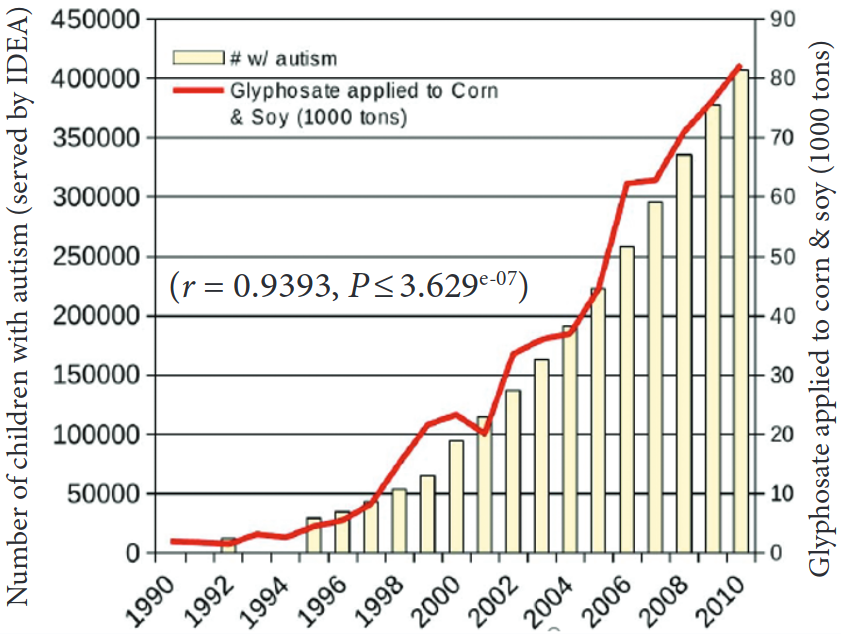
\includegraphics[width=\linewidth]{img/autisme_glyphosate.png}
		\caption[Relation entre autisme et utilisation de glyphosate.]{Relation entre autisme et utilisation de glyphosate, d'après \cite[Figure 2, p. 51]{shaw_elevated_2017} \label{fig:autisme-glyphosate}}
	\end{minipage} \hfill
	\begin{minipage}[b]{.46\linewidth}
		\centering
		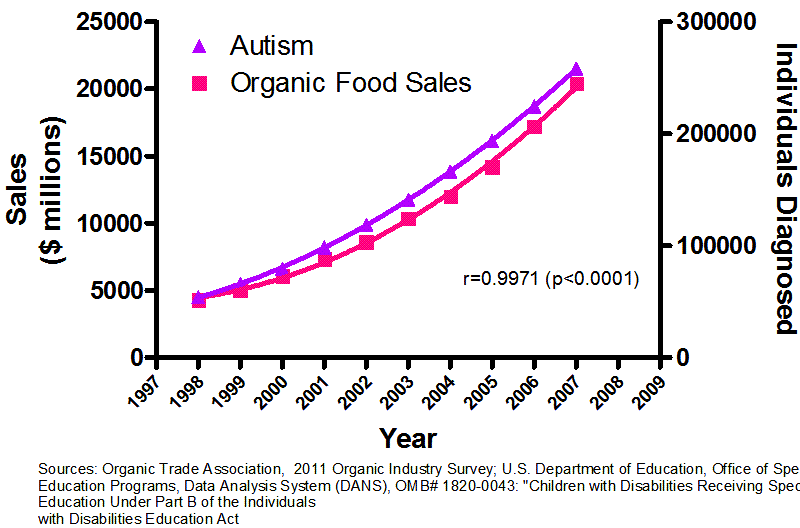
\includegraphics[width=\linewidth]{img/autisme_bio.png}
		\caption[Relation entre autisme et vente d'aliments \og bio\fg{}.]{Relation entre autisme et vente d'aliments \og bio\fg{}, d'après \og jasonp55\fg{}, 2012.}
		\label{fig:autisme-bio}
	\end{minipage}
\end{figure}

En termes de qualité de l'ajustement, le second modèle est meilleur : son coefficient de corrélation est de $0.997$ quand celui du premier ne vaut que $0.939$.
En dehors du principe statistique qui veut que causalité et corrélation ne soient pas équivalents, cet exemple illustre la nécessité d'apporter un éclairage en termes de plausibilité dans l'évaluation.
Tout épidémiologiste pourra en effet rejeter les conclusions du second graphique en se basant sur son intuition face à l'absence de relation empirique, au niveau individuel, entre autisme et alimentation biologique.
Cet exemple, trivial, illustre le besoin d'une évaluation basée sur la plausibilité, quand bien même une mesure de la validité aurait déjà été effectuée et jugée concluante.

C'est à cette évaluation de plausibilité que correspond, dans les \cref{fig:schema_kluegl,fig:schema_evaludationl} notamment, l'étape de \og \textit{face validation}\fg{}.
L'utilisation très polysémique -- et donc contradictoire -- de ce terme, et les importants débats autour de son usage ayant poussé à sa désuétude
\footnote{
	\cite[205]{mosier_critical_1947} recommande même son abandon : \og Since the term ''face validity'' has become overlaid with a high degree of emotional content and since its referents are not only highly ambiguous but lead to widely divergent conclusions, it is recommended that the term be abandoned.\fg{}
}, on le retrouve pourtant au cœur de l'un des articles fondateurs de l'évaluation de modèles de simulation, où \citeauthor{hermann_validation_1967} le définit ainsi :

\begin{quotation}
	\noindent \og
	Face validity is a surface or initial impression of a simulation or game's realism.
	Probably no approach to model validity is reported more frequently than the subjective estimates of experimenters, observers, or human participants as to the correspondence between the model's operation and their perception of the actual phenomena which the game or simulation represent.
	[...]\\
	Face validity can be a significant part of a validity strategy.
	A quick impression that "things don't seem right" may be the only validity check possible during the actual operation of a game or simulation.
	Such validity judgments and their evaluation may also be part of the learning experience provided by operating models designed for instructional purposes.
	\fg{}\\
	\mbox{}~ \hfill \textcite[221]{hermann_validation_1967}
\end{quotation}

Quelques années plus tard, on en trouve une définition plus succincte chez un des fondateurs de l'évaluation de modèles : \og Face validity is asking people knowledgeable about the system whether the model is reasonable.\fg{} \autocite[500]{sargent_validation_1979}.
Cette définition introduit un aspect qui nous semble important en matière de \textit{face validation} : il ne s'agit pas de faire évaluer la plausibilité d'un modèle par un quelconque examinateur, mais bel et bien par un expert du sujet modélisé\footnote{
	On retrouve l'expression de \og people knowledgeable about the system\fg{} chez \textcite[130]{balci_validation_1994}, et \textcite[2]{kennedy_verification_2006} parlent de \og domain experts\fg{}.
}.
Ce type d'évaluation n'a donc pas uniquement vocation à démasquer des comportements contre-intuitifs, mais bel et bien à faire expertiser, par un thématicien, le déroulement et l'aboutissement d'un modèle de simulation.

Il a fallu attendre la relative démocratisation des plate-formes de modélisation à base d'agents pour qu'une auteure, \citeauthor{klugl_validation_2008}, se penche véritablement sur l'identification et l'explicitation de la \textit{face validity}, et en donne une définition plus précise, mais englobante car centrée sur les usages plus que sur la méthode en elle-même :

\begin{quotation}
	\noindent \og
	Face validity can be seen as the result of face validation. Under this paradigm I want to subsume all methods that rely on natural human intelligence.
	Examples are structured walk-through, expert assessments of descriptions, animations or results.
	Thus, face validity shows that processes and outcomes are reasonable and plausible within the frame of theoretic basis and implicit knowledge of system experts or stake-holder.
	Face validation may be applied from the early phases of the simulation study under the umbrella of conceptual validations.
	It is often also called plausibility checking.
	[...]\\
	Face validation usually plays an important role during model design.
	All tests based on reviews, audits, involving presentation and justification of assumptions and model structure are used for reaching this form of plausibility.
	\fg{}\\
	\mbox{}~ \hfill \textcite[39--41]{klugl_validation_2008}
\end{quotation}


La description des méthodes possibles menant à cette évaluation n'est pas en reste non plus dans cet article, puisque l'auteur identifie trois familles de cette \textit{face validation}, chacune pouvant être menée par des experts différents \footnote{
	L'énumération qui suit est une traduction libre et une reformulation partielle de \textcite[41-42]{klugl_validation_2008}
} :

\paragraph{Composantes de la \textit{face validation}.}\label{par:composantes-face-validation}
\begin{itemize}
	\item \textbf{Évaluation du déroulement.} Ce type d'évaluation vise à analyser le déroulement d'une simulation dans son ensemble.
	Il s'agit ici de juger de la plausibilité des dynamiques (à l'échelle du système dans son ensemble, ou de composantes de celui-ci) reproduites dans la simulation, via une observation en direct de la simulation.
	
	\item \textbf{Évaluation des sorties.} Cette approche consiste plutôt à une évaluation qualitative des sorties produites par la simulation.
	Cela peut prendre la forme de vérifications des valeurs (approche que l'on retrouve dans les méthodes d'évaluation plus formelles, via une automatisation de ces types d'évaluation) par un expert, mais aussi d'analyse des covariations et évolutions temporelles de différents indicateurs de sortie.
	L'évaluation des sorties peut être appliquée sur le système modélisé dans son ensemble, mais aussi au niveau des types d'agents mobilisés.
	
	\item \textbf{Évaluation \og immersive\fg{}.} Il s'agit ici d'évaluer le modèle au travers de la vraisemblance des actions et réactions individuelles des agents qui y interagissent.
	L'accent est donc mis sur la plausibilité du comportement des agents (niveau micro), plus que sur celle des dynamiques macroscopiques résultantes.
	Les experts de ces deux niveaux d'observation peuvent être différents (un psychologue spécialiste des réactions individuelles en cas d'incident ne peut porter un jugement de même niveau qu'un physicien spécialisé dans les dynamiques de foules par exemple), et il faut donc, à chaque niveau d'observation du modèle, faire intervenir un expert adéquat.
\end{itemize}


Pour l'auteur, ces trois approches d'évaluation sont complémentaires et s'inscrivent dans des temporalités différentes de la phase de vie du modèle.
Elle encourage ainsi plutôt à mener l'évaluation des sorties après les deux autres, puisque ces dernières sont comparativement moins coûteuses en termes de calcul \autocite[42]{klugl_validation_2008}.

Il nous semble que si les deux premières approches sont applicables à tout modèle, l'évaluation immersive comporte un postulat lourd sur la plausibilité des trajectoires individuelles.
Cela se prête bien à de nombreux modèles où les agents représentent des humains dotés de comportements rationnels, ou encore des particules dont la trajectoire individuelle est prévisible en dehors des effets d'interaction.
Toutefois, tout un pan de la modélisation en géographie repose sur des agents non anthropomorphiques, ou encore sur des entités primaires dont seules les interactions ont vocation à faire émerger un comportement d'ensemble.
Dans le cas de SimFeodal par exemple (\hl{ref chap2}), les comportements individuels des foyers paysans ne reposent pas sur des hypothèses de vraisemblance :
	le foyer paysan qui se déplace de villes en villes, parfois en faisant des allers-retours, au cours des 300 ans modélisés, ne s'appuie sur aucune connaissance empirique, et tendrait même à contrevenir aux connaissances expertes de la mobilité résidentielle des foyers paysans médiévaux.
On pourrait y voir une \og méta-plausibilité\fg{} inter-générationnelle, mais il serait difficile de l'interpréter et surtout de la différencier d'autres comportements de foyers paysans.
Le suivi d'un foyer paysan, isolé de ses co-agents, au cours du déroulement du modèle, par un expert thématicien, n'est donc pas sujet à évaluation, au contraire du suivi des structures spatiales de niveau macroscopique engendrées par cette accumulation de déplacements.

L'évaluation immersive, bien que peu adaptée à certains types de modèles, peut toutefois s'avérer de manière universelle utile en matière d'évaluation interne, dans un aspect de \og débugage\fg{}.
Même si les réactions et attributs des agents ne reproduisent pas une connaissance experte, leur observation peut toujours servir au modélisateur pour vérifier l'absence de valeurs aberrantes ou encore la juste activation de chacun des mécanismes.



\subsubsection{Limites}

Comme mentionné auparavant (\ref{par:quelle-eval-quel-modeles}), pour de nombreux auteurs \autocite{hermann_validation_1967, balci_validation_1994, kennedy_verification_2006}, la \textit{face validation} ne peut qu'être une étape préalable à des méthodes d'évaluation plus quantitatives et formelles.
Les raisons données sont souvent le manque d'objectivité d'une démarche fondamentalement basée sur l'expertise et l'impression.
Parmi ces auteurs, \citeauthor{hermann_validation_1967} est sans doute celui qui se montre le plus méfiant vis-à-vis de la pratique de la \textit{face validation}, en en pointant plusieurs limites :

\begin{quotation}
	\noindent \og
	Although face validity has value in the early stages of model building or for quick checks during actual operation, its severe limitations should be recognized.
	Sometimes the experimenter will not know what behaviors are "realistic" because of his limited experience observing the actual phenomena.
	Participants can become interested and highly motivated in an incorrect representation of the desired environment.
	If the simulation involves the substitution of one property for another, some features may appear quite unreal and yet replicate the performance of the reference system for which the simulation was designed.
	The acceptance of face validity as a rough, first approximation might be improved if the simulator explicitly stated in advance what observations would constitute indications that an aspect of the observable universe had been successfully captured.
	In summary, face validity in its usual form suffers from the lack of explicit validity criteria.
	\fg{}\\
	\mbox{}~ \hfill \textcite[222]{hermann_validation_1967}
\end{quotation}

Ces réserves nous semblent être autant de pistes pour justifier de l'intérêt d'une démarche scientifique de \textit{face validation}. En reprenant les critiques dans l'ordre énoncé par l'auteur, on peut y répondre ainsi :
\begin{itemize}
	\item \textbf{Manque de connaissance experte.}
	Cette première remarque nous apparaît comme quelque peu biaisée : si l'on confie une évaluation experte à des non experts, naturellement, cela ne peut déboucher sur une évaluation correcte du modèle.
	Cela est d'ailleurs applicable quelle que soit la méthode d'évaluation : une expertise ne vaut que par la qualité de l'expert.
	De manière plus nuancée, on notera d'ailleurs que cette phrase montre ici l'absence d'un élément de définition de la \textit{face validation} partagé par les autres auteurs :
	\citeauthor{hermann_validation_1967} considère par là que c'est au modélisateur uniquement de mener cette phase d'évaluation, alors que la littérature s'entend quant au fait que ce rôle échoit à des experts.
	Ce faisant, \citeauthor{hermann_validation_1967} se positionne dans la logique de construction de modèles par des modélisateurs, sans apport des thématiciens, et donc dans l'approche classique de séparation forte entre ces deux acteurs indispensables du modèle (voir \hl{chapitre 1, prestation vs co-construction}).
	
	\item \textbf{Invraisemblance de certains comportements.}
	\citeauthor{hermann_validation_1967} met en avant que dans un modèle, tous les mécanismes n'ont pas vocation à être vraisemblables.
	Ainsi, en mentionnant ces \og propriétés de substitutions\fg{}, il rappelle un élément important d'une évaluation, quelle qu'en soit la méthode.
	On ne doit et ne peut en effet juger de la plausibilité que des aspects du modèle qui cherchent à reproduire un comportement plausible.
	Il nous semble qu'ici aussi, la critique de l'auteur revient à ignorer l'importance du dialogue entre modélisateur et évaluateur, tout en présumant que l'évaluateur ne serait pas le modélisateur.
	Si le modélisateur connaît les \og substitutions\fg{} opérées dans le modèle, il se gardera donc bien de juger de leur vraisemblance.
	\textit{A contrario}, un expert thématicien pourrait être étonné par certains comportements micro, dans la mesure où il ne connaîtrait pas les correspondances entre éléments du modèle et éléments du système modélisé.
	Là encore, cette limite repose donc surtout sur le choix d'un mode de construction isolé, c'est-à-dire n'impliquant pas et le thématicien et le modélisateur.
	Plus généralement, cette limite est présente s'il n'y a pas d'explicitation des \og substitutions\fg{} implémentées, c'est-à-dire de la correspondance entre le domaine conceptuel et le domaine du modèle implémenté : le niveau attendu de plausibilité individuelle de chaque comportement doit être décidé pendant la construction du modèle.
	
	\item \textbf{Explicitation préalable des objectifs.}
	La dernière remarque de cette citation nous semble, sans conteste, être la plus importante et la plus juste.
	L'auteur note ainsi que la \textit{face validation} ne peut constituer une méthode d'évaluation adaptée si l'on ne spécifie pas, en amont, les critères qu'elle doit s'attacher à examiner.
	C'est là encore vrai de toutes les méthodes d'évaluation, mais nous souscrivons aux remarques de \citeauthor{hermann_validation_1967} quant à l'importance primordiale que cela revêt pour la \textit{face validation}.
	En matière de plausibilité, on pourrait ainsi, comme cela nous semble souvent être le cas, se contenter d'évaluer \og à chaud\fg{} les différentes dynamiques et sorties d'un modèle, sans s'encombrer d'une démarche, ou feuille de route, spécifique.
	Le risque est alors d'introduire encore plus de subjectivité dans cette analyse, et en particulier de briser la capacité de reproductibilité ou de justification d'une évaluation :
	une évaluation peut être subjective tout en étant justifiée, appuyée par des arguments, et dès lors, reproductible si tant est que chacun de ces éléments soit explicités.
	Quand un modèle est évalué par une seule personne, par exemple un expert thématicien, la nécessité d'une telle démarche est peu visible, chacun étant en capacité d'estimer qu'il sera en mesure de justifier \textit{a posteriori} son évaluation.
	A contrario, quand un modèle résulte d'un travail collaboratif, qui plus est quand il implique plusieurs évaluateurs, les évaluations d'un même résultat peuvent varier.
	Il est donc indispensable de les expliciter autant que possible, et pour se prémunir d'un travail gigantesque d'analyse postérieure des résultats tout autant que pour se doter d'un outil de discussion et de débat commun, il apparaît primordial de fixer une grille d'évaluation, ou, en d'autres termes, d'un ensemble de critères à observer.
	Cela ne limite aucunement la nécessaire subjectivité et complémentarité des évaluateurs experts, mais permet au contraire d'inscrire leurs discours dans un référentiel de comparabilité.
	
\end{itemize}

\subsubsection{Intérêts de la \textit{face validation}}

En dépit des limites identifiées ci-dessus, qui nous semblent surpassables à condition de définir une grille d'évaluation avec précision en amont, la \textit{face validation} présente de nombreux atouts en dehors de la facilité de sa mise en œuvre traditionnelle.

Là où H\textsc{ermann} et les auteurs classiques cantonnent la \textit{face validation} à une étape préalable à une véritable évaluation, K\textsc{lügl} justifie l'intérêt propre de cette démarche méthodologique, y compris dans les phases plus avancées de la démarche classique d'évaluation :

\begin{quotation}
	\noindent \og One may argue why face validity is need, when statistical validation is successfully done?
	Face validation assures that the processes and structures are reasonable for a human expert.
	Especially, when there is (semi-)automatic calibration of a simulation that is used in combination with statistical validation, a careful check of plausibly is necessary.
	This is in general true for all kinds of simulation, but it is particularly important for agent-based simulations.[...]
	
	\noindent Although face validation may be informal and inconsistent, but it at least results in plausibility of modeled processes.
	Our experience with modeling and simulation in many interdisciplinary projects showed that even the formulation of a plausible model supports theory building and future empirical research.\fg{}\\
	\mbox{}~ \hfill \textcite[40;43]{klugl_validation_2008}
\end{quotation}


Pour l'auteure, la face validation complète ainsi d'autres méthodes d'évaluations mieux considérées, et nous irons même plus loin en considérant que chacune de ces méthodes peut potentiellement être améliorée en la conjuguant à une analyse de plausibilité visuelle de ses résultats.

On notera d'ailleurs que chez B\textsc{alci}, dans une analyse de l'applicabilité des méthodes de \og VV\&T\fg{} (\textit{Validation, Verification and Testing techniques}) aux différentes phases du cycle de vie d'un modèle, seules 5 techniques\footnote{
	Il s'agit systématiquement de méthodes \og informelles\fg{} : 
	(1) La vérification de la documentation (\textit{Documentation Checking}; (2) la \textit{Face Validation}; (3) les inspections de code; (4) les \og revues\fg{} de modèle (\textit{Reviews}) et enfin (5) les \og procédures pas à pas\fg{} d'évaluation (\textit{walkthrough}).
} (sur 77 analysées) présentent la caractéristique d'être mobilisables à chacune de ces phases.
Pour obtenir cette information, nous avons croisé plusieurs travaux de \textsc{Balci}.
Dans un premier article \autocite{balci_verification_1997}, cet auteur présente toutes les méthodes de VV\&T qu'il a identifié, et il les catégorise en quatre catégories.
Chaque méthode peut ainsi être formelle, informelle, statique ou dynamique.
Nous avons tiré d'un second article \autocite{balci1998verification} un tableau présentant l'applicabilité de chacune de ces méthodes à l'une des 18 étapes du \og cycle de vie\fg{} des modèles de simulation qu'il identifie.
En numérisant ces deux informations, relatives aux catégories des méthodes et à leur applicabilité, nous avons pu créer une représentation graphique (\cref{fig:taxonomy_balci}) qui les croise.

\begin{figure}[H]
	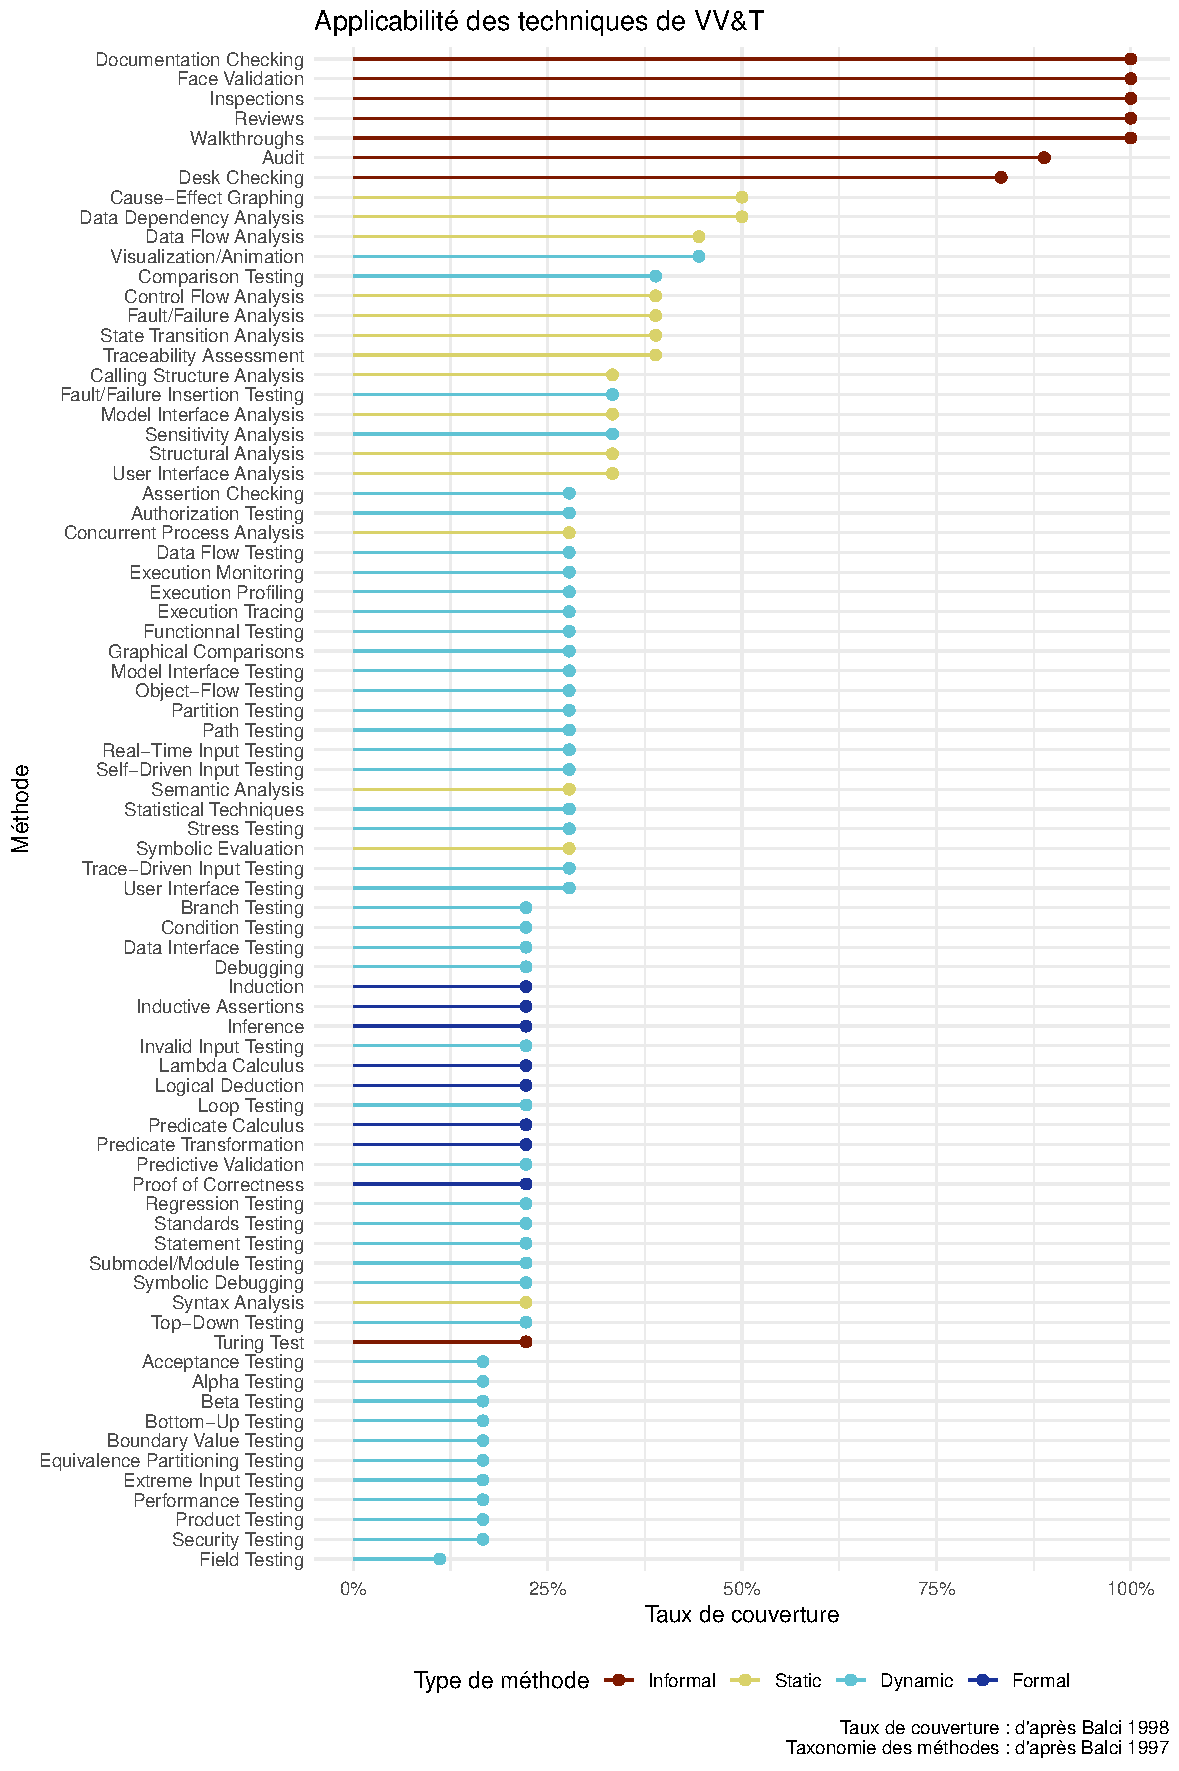
\includegraphics[width=\linewidth]{img/VVetT_Balci.pdf}
	\caption[Part des étapes de la cycle de vie d'un modèle pour lesquelles différentes méthodes de \og VV\&T\fg{} peuvent être mobilisées.]{Part des étapes de la cycle de vie d'un modèle pour lesquelles différentes méthodes de \og VV\&T\fg{} peuvent être mobilisées, selon le type de méthode (intitulés d'origine).\\
\textit{	Taxonomie des méthodes : d'après \textcite[Figure 2, p. 139]{balci_verification_1997} ; \\
	Taux de couverture : d'après \textcite[Table 3, pp. 45-47]{balci1998verification}.}}
	\label{fig:taxonomy_balci}
\end{figure}

Cette figure fait apparaître très nettement une \og hiérarchie\fg{} d'applicabilité des méthodes selon leur type : les méthodes informelles sont les plus souvent mobilisables, suivies par les méthodes statiques et certaines méthodes statiques.

\subsection{Vers une évaluation visuelle}

Au regard de ces éléments, il nous semble que l'utilité des approches de \textit{face validation} est assez largement prouvée.
C'est le cas que cette approche soit cantonnée à une phase préalable mineure ou au contraire à une bonne pratique plus générale, à mener lors de chacune des phases de construction et d'évaluation d'un modèle.

\subsubsection{Une démarche comparative}
Comme identifié en limites et en intérêts, il nous semble de plus que la \textit{face validation} souffre, en matière de réputation, d'un manque de clarification de la démarche qu'elle met en œuvre.
Nous considérons que dotée d'un protocole d'évaluation rigoureux, cette méthode peux constituer une alternative crédible à des méthodes d'évaluation plus répandues, par exemple les méthodes statistiques.
Ces dernières sont souvent basées sur l'analyse de l'écart entre des données empiriques et des données simulées, et cherchent à quantifier et à minimiser cet écart.
La \textit{face validation} procède à la même démarche comparative :
\begin{quotation}
		\noindent \og Face validation is a validation method that compares simuland behavior to model results. [...] Based on their knowledge of the simuland, the observers subjectively compare the behavior of the simuland as reflected in the simulation results with their knowledge of the behavior of the actual simuland under the same conditions, and judge whether the former is acceptably accurate. Differences between the simulation results and the experts' expectations may indicate model accuracy issues.
	\mbox{}~ \hfill \textcite[341]{petty2010verification}
\end{quotation}
Nous postulons que la démarche comparative que l'on retrouve dans l'évaluation statistique peut donc être appliquée sans recherche de quantification, c'est-à-dire en évaluant ces mêmes écarts de manière subjective et qualitative.
Dans les modèles descriptifs dotés de nombreux indicateurs non résumables, tel que SimFeodal (\hl{ref chap 2}), la comparaison terme à terme entre des valeurs numériques est potentiellement possible, mais non ordonnable et ne peut donc déboucher sur un indicateur unique (voir \cnameref{par:indicateurs-simfeodal}, \cpageref{par:indicateurs-simfeodal}).
De plus, les données empiriques qui permettraient de mener une comparaison sont trop lacunaires et incertaines pour être jugées suffisamment fiables pour évaluer le modèle.

\subsubsection{Une démarche rigoureuse} Nous pensons toutefois que ces carences quantitatives peuvent être compensés par les connaissances expertes des différents thématiciens impliqués dans la construction et l'évaluation d'un modèle.
Ainsi, dès lors que le processus d'évaluation est pensé en amont de son application, et qu'il est possible de parvenir à la création d'une grille d'analyse, c'est-à-dire à un protocole d'évaluation, il nous semble que la différence avec l'évaluation statistique est assez restreinte.
Pour évaluer les modèles du type de SimFeodal, nous considérons dès lors qu'il est tout à fait possible de faire reposer cette démarche sur une évaluation experte, s'inscrivant dans les logiques de \textit{face validation}, et en particulier de sa composante d'évaluation des sorties (voir \cnameref{par:composantes-face-validation}, \cpageref{par:composantes-face-validation}).

\subsubsection{Un nouveau terme ?} Dans la suite de cet ouvrage, nous nommerons cette approche \og \textbf{évaluation visuelle}\fg{}.
Ce terme n'est, à notre connaissance, que peu employé, et le semble surtout en études environnementales, par exemple pour définir une méthode de comptage d'espèces animales et végétales \autocite[par exemple][]{harmelin-vivien_evaluation_1985}.
Le pendant anglophone, la \og \textit{visual evaluation}\fg{}, semble s'inscrire dans le même champ disciplinaire \autocite[par exemple][]{horst_assessment_1984}, et paraît aussi assez faiblement utilisée dans un usage scientifique.
Dans l'usage qui en sera fait dans ce manuscrit, ce terme est forgé au regard de la \og \textit{face validation}\fg{} naturellement, et pourrait être confondu avec.
Il s'agit toutefois de s'éloigner de l'aspect \og apparence\fg{} présent dans le terme -- qui insiste donc sur une validité de façade --, pour embrasser au contraire la méthode visuelle.
Cette dernière a fait ses preuves -- dans de nombreux autres champs disciplinaires -- et constitue un pan non négligeable des méthodes d'analyse, et nous pensons donc adéquat d'en faire un usage argumenté dans le domaine de l'évaluation de modèles de simulations.
On notera un usage proche de cette dernière, appliquée aux modèles aussi, mais statistiques cette fois-ci, visant à l'évaluation visuelle de modèles de \og \textit{Data Science}\fg{}.
\textcite{eilers_its_2017} partagent le constat d'une utilité réelle de l'évaluation visuelle (intitulée \og Visual Model Evaluation\fg{} dans leur cas), et mettent une emphase particulière dans l'intérêt des intuitions que peuvent avoir les experts thématiques à la vue des résultats d'un modèle.
Pour ce faire, ils insistent sur l'intégration d'experts dans le processus d'évaluation, et sur le besoin de communications, lors de cette phase de travail, entre les modélisateurs et ces experts\footnote{
	\og Integrating these expert groups [data scientists and domain experts] to follow a common objective is still a major challenge today for a successful data science project in the industry and therefore a suitable field for information systems research.
	A collaborative analysis system addressing this issue should therefore focus on both aspects. It is important to most efficiently support human decision-makers with data-driven expert systems, and much research has been carried out in this area (Shim et al. 2002; Power 2008).
	But it is equally important that domain experts are also part of the system itself, e.g. by supporting data scientists with their domain knowledge when constructing the underlying models.
	A key success factor for this purpose is communication between different groups.\fg{} \autocite[2]{eilers_its_2017}
}.


\subsubsection{Définir l'évaluation visuelle} Pour définir cette évaluation visuelle, nous repartirons de la définition de la \textit{face validation} sur laquelle cette méthode s'appuie.

\paragraph{Définition.} Il s'agit d'évaluer, visuellement, la plausibilité du comportement d'un modèle à partir des données qu'il produit.
Cette plausibilité peut être entendue comme la correspondance entre le système modélisé et le modèle du système, correspondance s'exprimant en comparant les données en sortie de simulation -- et en les agrégeant au besoin pour tenir compte de la nécessaire réplication
\footnote{
	Cet aspect est discuté dans les chapitres \hl{1, 2 et 7}.
	En matière d'évaluation, tel que pointé par la majorité des auteurs cités dans cette sous-partie de chapitre, il est ainsi nécessaire de tenir compte de la variabilité d'un modèle, variabilité intrinsèque dans un modèle stochastique.
	Il n'est donc pas possible d'évaluer, visuellement ou non, un modèle stochastique sur la base d'une seule exécution. Au contraire, seule l'exécution d'un certain nombre de \textbf{réplications} (voir \hl{chapitre 1}) permet de s'assurer que le comportement évalué correspond bien au comportement habituel, ou tendanciel, du modèle.
} -- au comportement du système modélisé.
Cette correspondance doit être qualifiée avant de mener cette phase d'évaluation, c'est-à-dire qu'il est nécessaire de spécifier les critères d'observation et les réponses attendues.
Ces éléments, les critères d'évaluation, ne peuvent être formulés par n'importe qui : si le modélisateur autant qu'un expert externe peuvent les spécifier, il convient de s'assurer de l'expertise -- thématique et de la connaissance du système tel que modélisé -- de l'évaluateur.
On obtient ainsi un système à évaluer au filtre d'une grille d'analyse qualitative et basée sur le visuel.
Il devient alors possible d'apprécier l'écart le modèle et le système qu'il représente, sans chercher pour autant à quantifier ou à mesurer cet écart. 
Il s'agit en effet plutôt d'ordonner différentes versions ou paramétrages d'un modèle de simulation afin de juger de ceux qui semblent minimiser cet écart.

Un dernier point nous semble particulièrement appréciable dans ce recours à l'appréciation visuelle plutôt qu'à une mesure stricte de l'écart entre une situation estimée parfaite et une situation simulée.
C'est la capacité, humaine, à estimer semblable des configurations spatiales qui seraient jugées très différentes par une méthode de calcul quelconque.
Si l'on cherche par exemple à estimer l'écart entre un semis de point cible et un semis simulé, on peut mesurer l'écart comme, par exemple, une somme des écarts de chacun des points à celui qu'ils sont sensés représenter.
Un décallage minime, par exemple obtenu par translation horizontales de quelques dizaines de mètre sur un semis régional, engendrera alors une démultiplication des erreurs, alors même qu'un œil humain aurait jugé ces deux semis quasi-identiques.
En terme de configuration spatiale, la quantification peut ainsi amener à des contres interprétations dans l'analyse.
Dans le cadre d'un modèle comme SimFeodal où l'espace est important et qui plus est, théorique et aléatoire, et donc difficilement agrégeable (\hl{cf. chapitre 7}), le recours systématique à l'évaluation visuelle nous paraît alors indispensable.

\paragraph*{}Cette méthode, contrairement à d'autres, plus quantitatives, permet donc au final de tirer avantage des méthodes qualitatives telles que la \textit{face validation} -- par exemple la capacité d'évaluer un modèle qui ne reposerait que sur peu de données empiriques ou encore sur des données incertaines --, tout en se confortant à une démarche d'évaluation rigoureuse, loin de l'estimation \og au doigt mouillé\fg{} à laquelle peuvent donner lieu certaines méthodes reposant sur la plausibilité et l'estimation.

\subsubsection{Des critères pour l'évaluation visuelle : construire des indicateurs de sortie de simulation}

Dans la présentation de la démarche d'évaluation visuelle, nous précisions que pour que cette évaluation qualitative et experte soit rigoureuse, il était nécessaire de fixer des objectifs de manière préalable, et d'en expliciter la teneur autant que possible.

Pour l'évaluation de SimFeodal, face à la multiplicité des attentes thématiques vis-à-vis du modèle, nous avons choisi de mobiliser à cet effet des \og indicateurs de sortie\fg{}.
Ceux-ci relèvent du domaine de la simulation et leur évaluation doit être guidée par les connaissances empiriques, formalisées au sein d'\og indices empiriques\fg{} qui correspondent à ces indicateurs.

Pour finir de décrire la démarche d'évaluation de SimFeodal, il reste donc à définir plus précisément ces composantes de l'évaluation, ainsi qu'à expliciter les objectifs fixés pour chacun des indicateurs que l'on va construire.

\let\orisectionmark\sectionmark
\renewcommand\sectionmark[1]{}%
\section{Une grille d'analyse composée d'indicateurs de sortie}
\orisectionmark{Les indicateurs de sortie}
\let\sectionmark\orisectionmark

Le modèle SimFeodal présenté dans le \hl{chapitre 2} correspond à la \og version 6.3 \fg{} du modèle, c'est-à-dire qu'il en constitue une version qui n'est ni la première, ni sans doute la dernière dans cette expérience de co-construction interdisciplinaire de modèle qui s'inscrit résolument dans le temps long.
L'ensemble des mécanismes figurant dans le modèle conceptuel ont été implémentés mais l'ensemble des liens, interactions et valeurs de paramètres ne sont pas encore stabilisés.
De ce fait les résultats des simulations ne répondent pas toujours complètement aux attentes définies dans le \hl{chapitre 2}.

Si l'on a déjà décrit le principal objectif du modèle dans le chapitre précédent (celui de comprendre les mécanismes sous-jacents au processus de polarisation qui s'est déroulé entre 800 et 1100), il convient ici d'expliciter comment les résultats d'un tel processus peuvent être saisis.
Ceux-ci sont en effet nombreux et hétérogènes, concernant aussi bien des concentrations de foyers paysans que l'émergence de pôles.
Certains sont centraux, d'autres secondaires, et le modélisateur a des attentes relativement aux résultats qui devraient être obtenus en fin de simulation.
La description précise de ces attentes se révèle importante dans le cadre du paramétrage -- et de l'ensemble des étapes de la vie du modèle -- de SimFeodal.

Une telle description repose sur la construction d'\og{}indices empiriques\fg{} et d'\og{}indicateurs de sortie de simulation\fg{} qui vont permettre de rendre compte des résultats des simulations.
Il s'agira d'exprimer les attentes sous formes de critères relatifs à ces indicateurs de sortie de simulation.

Dans cette partie, on explicitera d'abord le sens que l'on prête à ces \og indices empiriques \fg{} et \og d'indicateurs de sortie de simulation\fg{}.
Ces indices et indicateurs sont nombreux, certains sont multivariés, et il s'agira donc de présenter des méthodes visant à réduire la complexité de ces indicateurs de sortie, en adoptant une démarche proche de ce qui se fait en statistiques : réduction de dimensionnalité et/ou catégorisation et hiérarchisation de ces indicateurs.
L'utilisation de ces méthodes permettra, seule, de décrire et qualifier le comportement du modèle SimFeodal tel qu'il a été décrit dans le chapitre précédent, avant d'en analyser les résultats par ce biais dans le \hl{chapitre 6}.

\subsection{Indices et indicateurs}\label{subsec:indices-indicateurs}

On attend d'un modèle, sans entrer encore dans le détail, qu'il reproduise au moins les grands traits de l'élément empirique dont il est sensé rendre compte.
Ces grands traits peuvent s'entendre de multiples manières, et se formaliser avec encore plus d'approches.
Ici, nous avons souhaité proposer une dichotomie simple entre le domaine de l'empirique et celui de la simulation, en systématisant l'usage d'un vocabulaire qui est souvent employé de manière plurielle.
Pour être en mesure d'évaluer la vraisemblance du comportement reproduit par le modèle sur le plan empirique, il est nécessaire de mettre en correspondance des éléments empiriques et des éléments issus de la simulation.
Nous caractérisons ces éléments en deux grands ensembles :
(1) \textbf{les indices empiriques}, éléments quantifiables ou au moins descriptibles émanant du domaine empirique, et (2) \textbf{les indicateurs de sortie}, variables informatiques produites par le modèle de simulation et devant pouvoir être comparés à chacun des indices empiriques.
La \cref{fig:schema_indices} reprend, sous forme de schéma ontologique synthétique, ces deux ensembles de mesures, explicitant le vocabulaire mobilisé dans cette partie.

\begin{figure}[H]
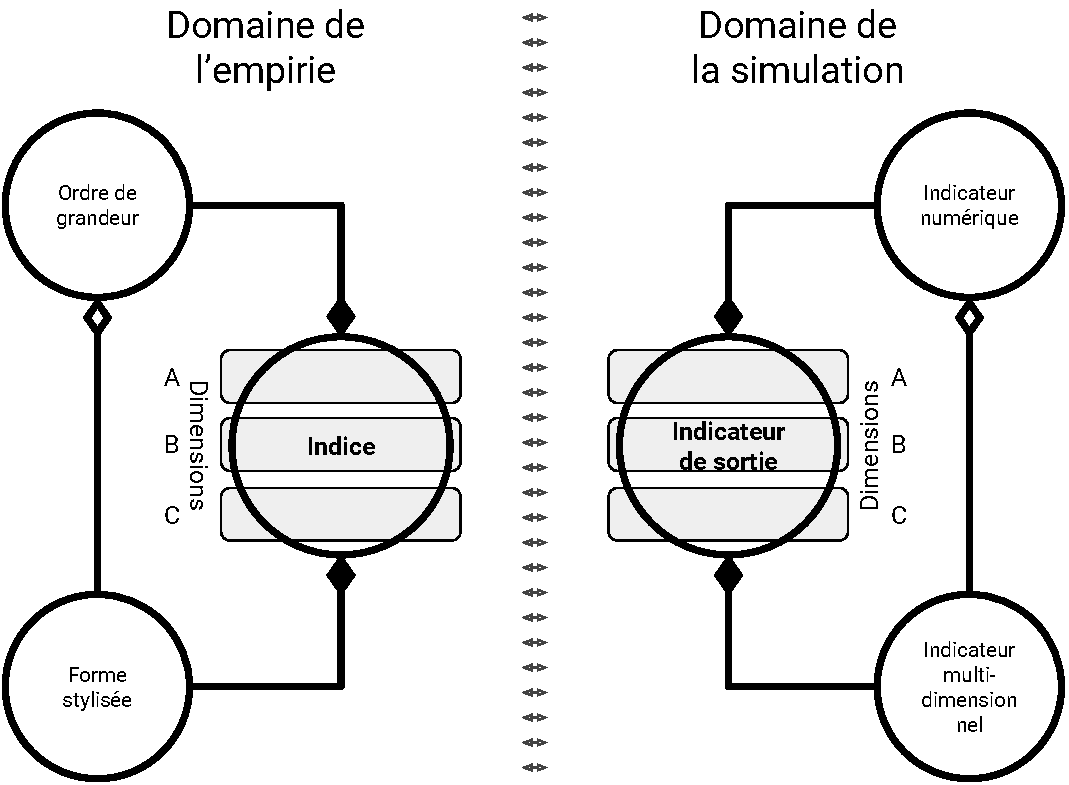
\includegraphics[width=\linewidth]{img/schema_indice_indicateur.pdf}
\caption[Schéma de synthèse des correspondances entre mesures empiriques et simulées.]{Schéma de synthèse des correspondances entre mesures relevant du domaine empirique et mesures issues des simulations pour l'évaluation du modèle SimFeodal
%\footnotemark.
}
\label{fig:schema_indices}
\end{figure}
%\footnotetext{
%	La correspondance des éléments est représentée par une symétrie axiale, entre d'un côté des \og indices empiriques\fg{} et de l'autre des \og indicateurs de sortie de simulation\fg{}.
%	Les losanges pleins désignent une relation de composition :
%	un \og indice empirique\fg{} est soit un ordre de grandeur, soit une forme stylisée.
%	Les losanges vides indiquent une relation d'agrégation :
%	une forme stylisée est une agrégation d'ordres de grandeurs.
%	Les dimensions (A à C) regroupent des indices (et les indicateurs qui leur correspondent) qui peuvent être de plusieurs types, et sont elles aussi comparables et en correspondance entre les domaines.
%}

Dans cette figure, on représente au moyen d'une symétrie axiale la correspondance entre le \textbf{domaine empirique} et le \textbf{domaine de la simulation}.
Les \textbf{indicateurs de sortie} sont donc la correspondance simulée des \textbf{indices} du domaine empirique.
Indices et indicateurs de sortie sont catégorisés selon des \textbf{dimensions} (A, B, C) qui correspondent aux processus que l'on cherche à modéliser : la polarisation du système de peuplement, sa hiérarchisation, sa fixation, etc.
Les dimensions sont donc composées\footnote{
	Les losanges noirs marquent une relation de composition dans le formalisme UML, repris dans ce schéma.
	La position du losange indique le sens de la relation : les indices sont composés d'ordres de grandeur et de formes stylisées.
} d'un ensemble d'indices, pour la partie empirique, et des indicateurs de sortie de simulation correspondants.

Les indices empiriques peuvent être de deux formes.
Nous nommons la forme la plus simple \og \textbf{ordre de grandeur}\fg{}.
Ces indices expriment donc une valeur observée, connue avec plus ou moins de certitude (d'où le terme d'ordre de grandeur), qui trouvera une correspondance dans le domaine simulé sous la forme d'un \textbf{indicateur numérique}.
D'autres indices ont une forme plus complexe, reposant sur l'agrégation\footnote{
En UML, un losange vide symbolise les relations d'agrégation : plusieurs ordres de grandeurs sont nécessaires pour définir une forme stylisée.
} de plusieurs ordres de grandeur, et on les nomme \og formes stylisés\fg{}, par analogie aux faits stylisés déjà décrits.
Dans le domaine de la simulation, les indicateurs de sortie correspondant sont appelés \og \textbf{indicateurs multidimensionnels}\fg{}, pour appuyer l'idée qu'ils sont constitués de plusieurs indicateurs numériques.

On peut illustrer cela avec un exemple tiré de SimFeodal.
Dans le domaine empirique, on sait que la part de l'habitat rural dispersé tend à diminuer au cours de la période, depuis environ 95\% jusqu'à environ 20\%.
C'est notamment l'un des indices du processus de polarisation, qui constitue une dimension d'analyse.
Ces deux valeurs sont des indices empiriques, de type \og ordre de grandeur\fg{}.
Dans le modèle de simulation, on a un indicateur de sortie correspondant qui correspond au taux de foyers paysans isolés.
Le taux de foyers paysans isolés en début de simulation est un indicateur numérique, de même que celui en fin de simulation.
La forme de la courbe d'évolution du taux de foyers paysans isolés au cours de la simulation est un indicateur multi-dimensionnel : elle repose sur une succession d'indicateurs numériques que sont le relevé du taux à chaque pas de temps.
Cette forme de courbe peut être évalué au regard de la forme stylisée, dans le domaine empirique, sur laquelle est s'appuie.
On sait que la part de l'habitat rural diminue régulièrement au cours du temps, et on évaluera donc, pour cette dimension (la polarisation), la capacité du modèle à reproduire un processus de polarisation semblable à celui observé par le biais de la forme stylisé \og diminution régulière de la part de l'habitat rural dispersé\fg{}.


\subsubsection{Les indices empiriques.}

Afin d'évaluer la capacité du modèle à reproduire un phénomène observé, il est nécessaire de disposer dans le domaine empirique, de \og points de repère\fg{}.
Selon les modèles, ceux-ci peuvent revêtir de multiples formes et relever de l'ensemble des échelles spatiales et temporelles que l'on choisit de mettre en scène dans le modèle.
Leur point commun est qu'ils doivent pouvoir être mesurés, au sens le plus large, c'est-à-dire être en capacité d'être reproduits et comparables avec d'autres mesures.
Dans cette étude, on a décidé de qualifier ces points de repère d'\og\textbf{indices empiriques}\fg{} et de les regrouper en deux catégories basées sur la précision avec laquelle ils peuvent être décrits et non sur la précision de leur connaissance, cf. \cref{sssec:incertitude}.
La \cref{fig:schema_indices} illustre cette catégorisation entre la première catégorie -- les ordres de grandeur -- et la seconde -- les formes stylisées --.

\paragraph{Ordres de grandeur.}
La première catégorie est constituée d'\textbf{ordres de grandeurs} empiriques estimés -- avec une précision plus ou moins importante (\hl{cf. tableau 3 p. 317 du chap. TMD, à reproduire dans chap 2}).
Certaines valeurs empiriques sont ainsi connues, que ce soit d'après des sources primaires ou secondaires, et peuvent ainsi constituer des indices.
Par exemple, on connaît avec quasi-certitude le nombre d'églises paroissiales de la région Touraine en 1100.
D'autres valeurs empiriques sont en revanche issues d'estimations.
Tel est le cas, par exemple, du taux de foyers paysans isolés en fin de période.
Celui-ci ne peut être renseigné par des sources primaires et il a donc été nécessaire de l'estimer à partir de sources secondaires et en menant des extrapolations.
Il est cependant possible de construire des indicateurs de sortie de simulation offrant une correspondance presque exacte avec ces différents indices observés ou estimés (cf. \cnameref{par:correspondance}, p. \pageref{par:correspondance}).
Il est dès lors possible de mener une comparaison entre données observées/estimées et données simulées.
Ces ordres de grandeur peuvent ainsi participer à l'évaluation du comportement du modèle simulé.

\paragraph{Faits et formes stylisés.}
La seconde catégorie d'indices empiriques est moins précise et ne repose pas sur une valeur observable ou estimable, mais plutôt sur la connaissance experte d'un phénomène.
Il s'agit des \og \textbf{faits stylisés}\fg{}\footnote{
	Définis ainsi par \autocite{livet2014diversite}: \og
	Un ``fait stylisé'' est une présentation simplifiée (i.e. taux, ratio ou écart, structure spatiale) d'une régularité empirique sur l'observation de laquelle il y a un large accord.
	Le terme a été popularisé en économie par Nicholas Kaldor (1961).[Les] faits stylisés peuvent être construits de la manière suivante :
	1) en partant du domaine empirique, on identifie des relations saillantes ;
	2) on opère quelques simplifications qui permettent d'inclure formellement ces relations dans des modèles ;
	3) une fois admis que ces simplifications ne faussent pas trop les choses, on érige ces relations à la fois simplificatrices et formalisables au rang de `` faits stylisés'', dont les concepts théoriques doivent rendre compte.\fg{}
}, qui rendent davantage compte d'une tendance dans la forme d'une relation ou d'une organisation que d'un ordre de grandeur.
On fait un large usage de ces faits stylisés en économie, mais aussi en géographie, par exemple quand on qualifie la tendance des systèmes de peuplement à se hiérarchiser.
La valeur de la pente associée à la courbe rang-taille d'un système de villes a ainsi été décrite comme tendant vers $1$ à mesure que le système évolue et se hiérarchise (\cite{berry_city_2012}, in \cite[\S9]{pumain_multilevel_2015})\footnote{
	Notons que les auteurs de \textcite{pumain_multilevel_2015} nuancent cette affirmation, en montrant empiriquement que les pentes convergent vers des valeurs supérieures ou inférieures à 1 en fonction de l'ancienneté de l'intégration des systèmes de ville considérés \autocite{cura_old_2017}.
}.
De la même manière, le modèle de transition démographique d'Adolphe Landry est un fait stylisé, énoncé à partir de l'observation de nombreuses récurrences de l'évolution des populations d'un pays en fonction de leurs taux de natalité et de mortalité.
Ces exemples montrent qu'au sein des faits stylisés, il y a une certaine diversité quant à la précision de leurs énoncés.
On peut ainsi quantifier précisément la courbe d'une relation rang-taille et l'allure de son évolution dans le temps, au moyen de l'évolution du coefficient de sa pente, et ces indices empiriques sont le plus souvent communiqués dans la littérature.
Pour la transition démographique, on peut certes l'exprimer sous la forme d'une courbe logistique, mais les paramètres de cette courbe ne sont le plus souvent pas donnés dans les études thématiques.
Le fait stylisé \og transition démographique\fg{} est ainsi communiqué d'une manière moins précise que le fait stylisé \og hiérarchisation d'un système de villes\fg{}.

Dans notre cas d'étude, les faits stylisés sur lesquels on s'appuiera seront d'une part des \og allures\fg{} de courbes, temporelles (par exemple l'évolution dans le temps d'un indicateur tel que le taux de concentration des foyers paysans) ou liées à une composition de valeurs (par exemple la courbe rang-taille correspondant à la hiérarchie des agrégats), et d'autre part des formes de répartition spatiale (densité du semis d'églises paroissiales par exemple).
Notons que ces formes stylisées relèvent le plus souvent d'une agrégation ou d'une composition d'ordres de grandeurs (comme figuré dans la \cref{fig:schema_indices}) :
l'évolution dans le temps de la population, par exemple, correspond à un vecteur d'ordres de grandeur, c'est-à-dire à une succession de mesures de la quantité de population pour chaque date étudiée.

\subsubsection{Les indicateurs de sortie de simulation}

Les ordres de grandeur et formes stylisées évoqués  ci-dessus relèvent du domaine empirique, c'est-à-dire qu'on dispose de données ou de connaissances d'experts à leur sujet.
Afin de pouvoir les mobiliser pour évaluer la capacité du modèle à reproduire le phénomène d'intérêt, il est nécessaire de définir des \textbf{indicateurs de sortie} dans le modèle de simulation, c'est-à-dire des variables informatiques que l'on enregistrera durant l'exécution du modèle et que l'on pourra ensuite comparer aux indices empiriques définis.

\paragraph{Définition.}
Comme pour les indices empiriques qui sont leurs équivalents dans le domaine empirique, on peut définir les indicateurs de sortie de simulation, en distinguant des formes numériques simples (des scalaires), et des indicateurs plus complexes, multidimensionnels.
Ces derniers sont en effet nécessaires pour pouvoir confronter les sorties du modèle de simulation avec les formes stylisées identifiées dans le domaine empirique.
Chaque indice empirique doit ainsi se voir correspondre un indicateur de sortie (\cref{fig:schema_indices}).

\paragraph{Correspondance entre indicateurs de sortie de simulation et indices empiriques.}\label{par:correspondance}

La correspondance entre indicateurs et indices ne correspond pas toujours à une équivalence exacte.
En effet, si certains indicateurs peuvent trouver un équivalent strict dans le domaine empirique-- le nombre de châteaux connus à chaque date a un sens strictement équivalent au nombre de châteaux simulés par le modèle --, d'autres correspondances sont moins directes.

Il peut s'agir de correspondances ayant trait aux mêmes éléments de base et le passage de l'indicateur à l'indice résulte alors d'une simple conversion.
Par exemple, du point de vue empirique, on connaît à peu près les populations de la région étudiée au début et à la fin de la période.
Dans SimFeodal cependant, on ne modélise pas des individus en tant que tels, mais des foyers paysans.
Le nombre de foyers paysans simulé n'est pas directement comparable à la population estimée, mais en supposant une moyenne de 4 ou 5 habitants par foyer paysan, il est possible d'en déduire un nombre d'habitants.

Dans d'autres cas enfin, le décalage entre indicateurs et indices est plus important.
Il s'agit notamment de caractéristiques du système féodal que l'on sait importantes mais pour lesquelles on ne dispose pas de données facilement quantifiables.
La puissance militaire des seigneurs, par exemple, est complexe à quantifier.
On sait d'après les connaissances expertes que la hiérarchie des puissances était forte à l'époque étudiée, majoritairement dominée par deux seigneurs (les comtes de Tours et de Blois) et assortie d'une grande quantité de petits chevaliers.
On sait de plus qu'avec les liens de vassalité, les grands seigneurs disposaient des forces militaires des seigneurs qui leur étaient assujettis.
Dans le domaine empirique on ne dispose pas d'éléments plus précis pour quantifier la puissance militaire des seigneurs.
Dans le domaine du modèle, en revanche, on a défini un indicateur \og proxy\fg{} de cette puissance à partir du nombre de foyers paysans s'acquittant de droits à chaque seigneur.
De cette manière, on peut observer précisément en sortie de simulation la hiérarchie implicite entre les seigneurs reproduite par le modèle, avec une quantification de leurs puissances respectives.
Ces éléments peuvent être comparés aux connaissances empiriques sur ces rapports de puissance entre les seigneurs à différents moments de l'époque féodale.

Les correspondances entre indicateurs de sortie et indices empiriques sont ainsi de nature multiple, reflétant différents niveaux de proximité entre le concept mobilisé dans le modèle et ce qui est observable dans le domaine empirique :
	les châteaux, entités d'intérêt dans le modèle, ont un équivalent direct dans le domaine empirique (il s'agit d'entités facilement observables et des données historiques les concernant sont disponibles) alors que la puissance militaire des seigneurs, élément moteur dans le modèle, a conduit à utiliser une variable dans le modèle pour laquelle on ne dispose pas d'observations empiriques.

La création d'indicateurs de sortie correspondant aux indices empiriques permet donc de quantifier une information qui n'est pas forcément aisément quantifiable dans le domaine empirique.

\paragraph{Indicateur composite.}

La forme \og informatique\fg{} (numérique ou multi-dimensionnelle) des indicateurs de sortie permet de trouver des manières plus simples d'évaluer le modèle que d'observer l'ensemble des indicateurs.
Chaque indicateur étant numérique, il devient en effet possible de les combiner au sein d'indicateurs composites, résultant en quelques indicateurs synthétiques permettant une évaluation plus rapide des résultats d'une simulation.
Ces indicateurs composites sont très fréquemment utilisés en statistiques, permettant par exemple de résumer une information multidimensionnelle en un indicateur simple.
L'Indice de Développement Humain (IDH), par exemple, est un indicateur composite dépendant de l'espérance de vie à la naissance, du niveau d'éducation et du niveau de revenu de chacun des pays caractérisés.
On le trouve très souvent utilisé, parce qu'il permet de résumer le niveau de développement d'un pays en agrégeant trois dimensions majeures, l'aspect sanitaire, culturel et économique.

\paragraph{Fonction objectif.}

En renforçant cette logique de synthèse de plusieurs dimensions, on peut aller plus loin dans la définition d'un unique indicateur, parfois composite et synthétique, qui permet d'évaluer à lui seul la qualité de représentation d'un modèle.
On nomme d'ordinaire cet indicateur \og fonction objectif\fg{} (ou \og fonction de \textit{fitness}\fg{}).
C'est une pratique très fréquente, qui plus est dans le domaine de la simulation informatique en particulier sur des modèles de type \og KISS\fg{} (\hl{ref. chap 1 ou 2}).
Il s'agit alors de définir une \og fonction objectif\fg{}, parfois composée d'une pondération des quelques indicateurs composites qui auront été identifiés, ou plus simplement, basée sur une unique variable que l'on juge représentative de l'ensemble du modèle.

Être en mesure d'évaluer un modèle à l'aide d'un unique indicateur a des avantages majeurs en pratique.
Cela permet par exemple d'explorer et de paramétrer un modèle de simulation de manière entièrement automatique puisqu'on peut alors générer une cartographie simple des résultats du modèle en fonction des valeurs de paramètres utilisés \autocite[voir][par exemple]{cherel_beyond_2015}.

Ces indicateurs composites et synthétiques résultent d'une quantification des autres indicateurs (excluant donc les formes stylisées qui sont plus libres d'interprétation), et apportent un grand confort dans le paramétrage d'un modèle de simulation.

\paragraph{Quels types d'indicateurs pour SimFeodal ?}\label{par:indicateurs-simfeodal}

SimFeodal n'est pas adapté à de tels indicateurs, parce qu'une large partie des faits stylisés et ordres de grandeur mobilisés proviennent de connaissances expertes, et les thématiciens qui les ont consolidées rechignent à créer de tels indicateurs composites.
Ces derniers demandent en effet de pondérer précisement l'importance de chacun des indicateurs par rapport aux autres.
Pour pouvoir pondérer cette importance, il faudrait de plus que les différents indices empiriques mobilisés présentent le même niveau de certitude, et que les indicateurs de sortie aient des variabilités similaires.
Cela n'est le cas ni des indices empiriques sur lesquels SimFeodal s'appuie, ni des indicateurs de sortie que le modèle produit.

On aurait ainsi pu créer quelques indicateurs composites, mais ceux-ci n'auraient pas eu de véritable correspondance dans le champ empirique, les thématiciens ne faisant pas appel à des indices empiriques de telle sorte.
Un indicateur composite serait donc nécessairement \og hors-sol\fg{}, et qui plus est, perdrait beaucoup dans la finesse de description du système modélisé.

Par exemple, pour caractériser la polarisation du système de peuplement, il pourrait suffire de définir un indicateur composite fonction du niveau de concentration -- le taux de foyers paysans dispersés --, du nombre de pôles et de l'espacement moyen entre les agrégats.
Les valeurs de l'indicateur généré pourraient renseigner efficacement sur la capacité d'un ensemble de valeurs de paramètres à reproduire le phénomène de polarisation attendu.
Cette information serait cependant grossière, dans la mesure où seraient agrégées dans le groupe des \og simulations réussies\fg{} des configurations extrêmement diverses.
L'information fournie risquerait alors d'être très éloignée des connaissances empiriques des thématiciens :
une information multivariée ne peut pas toujours être résumée, en gardant tout son sens, par une seule variable (de manière univariée).

On a donc fait le choix d'évaluer SimFeodal en conservant des indicateurs de sortie \og simples\fg{}, c'est-à-dire ni composites ni exprimés sous forme de fonction objectif.
Ce choix a toutefois des implications majeures pour la méthodologie mise en place pour l'analyse des sorties de simulation.
Il est en effet bien plus simple d'analyser quelques indicateurs composites plutôt qu'un grand nombre d'indicateurs hétérogènes.

\subsection{Hiérarchiser et catégoriser les indicateurs}

SimFeodal s'appuie sur une dizaine d'indicateurs numériques, ainsi que sur plus d'une trentaine d'indicateurs multidimensionnels.
Tous ces indicateurs ne présentent pas le même degré de certitude, la même échelle d'observation, et surtout, le même niveau de précision sur les phénomènes modélisés.
À chaque changement dans le modèle, pour une évaluation complète de la capacité de cette version à reproduire les indices empiriques, il faudrait donc observer et analyser chacun de ces nombreux et divers indicateurs.
Dans le contexte du paramétrage d'un modèle s'appuyant sur une logique itérative et incrémentielle (voir \Cref{enc:incrementalite-indicateurs}), on imagine bien que cela n'est pas possible :
le nombre d'indicateurs est bien trop élevé pour avoir rapidement une vision globale de la qualité de représentation du modèle.
Il faut dès lors, comme pour toute analyse synthétique, concevoir une hiérarchie d'observation et d'utilisation des indicateurs :
il ne sera pas nécessaire d'analyser chacun des indicateurs dans la plupart des cas, seuls les indicateurs jugés plus importants pourront être analysés.
Les indicateurs de moindre importance ne seront mobilisés que pour départager des situations dont la différence ne serait pas suffisamment explicitée par l'usage des indicateurs principaux.

\subsubsection{Incertitude}\label{sssec:incertitude}
Dans le modèle de simulation, les indicateurs de sortie sont à analyser en tenant compte de la précision des indices qu'ils représentent.
Il ne faudra ainsi pas étudier la croissance du nombre d'agrégats au cours de la simulation de manière fine, par exemple en étudiant le coefficient directeur de la courbe, quand les données empiriques ne donne quasiment aucune information à ce sujet si ce n'est qu'il y a bien plus d'agrégats en fin de période qu'au début.
On peut vouloir quantifier la précision de ces données, par exemple à l'aide des méthodes développées dans le champ des observations floues et/ou incertaines (voir par exemple le travail de Cyril de Runz sur les données \og imparfaites\fg{} \autocite{de2008imperfection}).

Cette quantification de l'incertitude pourrait alors servir de base à l'établissement d'une hiérarchie des indicateurs :
on analyserait en premier lieu l'écart entre les ordres de grandeurs empiriques bien connus (\hl{cf. tableau du niveau de certitude des objectifs}) et les indicateurs calculés sur les données simulées.
Les ordres de grandeur plus incertains seraient analysés dans un second temps (augmentation de la charge fiscale entre 800 et 1100 par exemple), et les formes stylisées viendraient enfin clore cette hiérarchie d'indicateurs.

SimFeodal se caractérise d'une part par une très forte hétérogénéité dans les niveaux de connaissance des ordres de grandeurs et faits stylisés modélisés, et d'autre part, se voulant un modèle théorique (\hl{ref dans chap1}), \og coller aux données\fg{} à tout prix n'est pas la priorité.
La vraisemblance d'ensemble du modèle compte en effet bien plus que la précision de chacune de ses composantes.
Pour l'évaluation de SimFeodal, nous ne tiendrons compte de l'incertitude des indicateurs qu'au cas par cas, sans la mesurer de manière systématique et donc sans établir de hiérarchie à partir de cette incertitude.


\subsubsection{Catégoriser les indicateurs : définir des dimensions d'analyse}
En présence de plus d'une quarantaine d'indicateurs, il est nécessaire, \textit{a minima}, d'organiser leur analyse.
On a vu qu'il n'était pas justifié de mener cet ordonnancement à partir des propriétés intrinsèques des indicateurs du modèle.
Au contraire, et cela nous semble plus adapté pour un modèle à forte visée exploratoire et heuristique, la hiérarchisation des sorties du modèle doit suivre la hiérarchie implicite qui structure les hypothèses et objectifs du modèle en lui-même.
Ces hypothèses et objectifs sont multiples dans SimFeodal, et dès lors, une hiérarchie globale ne peut être définie.
Il convient donc de catégoriser les indices empiriques -- et les indicateurs de sortie de simulation leur correspondant --, avant de chercher à hiérarchiser ces indicateurs de manière globale.
La hiérarchisation des indicateurs se fera donc relativement à chacune de ces catégories.

La dynamique du système de peuplement que l’on cherche à reproduire sur la période IX$^e$-XII$^e$ siècle comprend trois processus (\hl{cf. chapitre 2}), que nous nommerons dimensions (voir \cref{fig:schema_indices}) :
(1) polarisation de l'habitat rural, (2) hiérarchisation du système de peuplement et (3) fixation des foyers paysans.
On peut s'appuyer sur ces trois dimensions pour caractériser les sorties du modèle, c'est-à-dire mener la confrontation entre indices empiriques et indicateurs de sortie.

On va répartir chacun des indicateurs dans la dimension qu'il sera le mieux en mesure de décrire.
Cette répartition n'a pas à être égale, chaque dimension pouvant s'appuyer sur un nombre différent d'indicateurs.
De même, chaque dimension sera composée d'indicateurs dotés d'une qualité de représentation ou d'un niveau de certitude hétérogène.
Le seul point commun des indicateurs de sortie de chaque dimension doit être thématique.
Les trois dimensions choisies -- polarisation, hiérarchisation et fixation --, et les indicateurs qui les caractérisent dans le modèle, sont dès lors considérés comme les trois dimensions d'analyse des sorties de SimFeodal.

\subsubsection{Hiérarchiser les indicateurs dans chaque dimension}\label{par:hierarchie_interne}
Chacune de ces dimensions s'applique à plusieurs types d'agents du modèle.
Pour définir la hiérarchie interne aux dimensions, on retiendra les agents les plus impactés par les dynamiques correspondant à ces dimensions :
la polarisation, par exemple, peut être observé depuis le point de vue de ce qui polarise (les attracteurs) tout autant que de ce qui est polarisé (les foyers paysans).

Pour trancher, on examinera d'abord un indicateur de sortie numérique, caractéristique de la structure dans son ensemble à son état final.
Les indicateurs de sortie représentatifs des dynamiques ayant mené à cette structure finale, par exemple les indicateurs multi-dimensionnels temporels, seront étudiés dans un second temps.
Dans cet exemple, on analysera donc dans un premier temps le résultat effectif de la polarisation, c'est-à-dire la concentration des foyers paysans en agrégats, avant d'observer dans un second temps la répartition et la diversité des attracteurs ayant entrainé ce phénomène.
On peut dès lors définir des \og indicateurs principaux\fg{} pour chaque dimension, représentatifs des grands traits structurels auxquels on souhaite aboutir en sortie de simulation, et des \og indicateurs secondaires\fg{}, permettant d'affiner l'évaluation de chacune de ces dimensions.

\subsubsection{Une hiérarchie mouvante}
Notons que l'analyse des indicateurs de sortie suit une hiérarchie parfois mouvante, et en tous les cas, assez peu quantifiable.
L'ordre d'observation des indicateurs est plutôt stable, mais l'importance que l'on portera à chacun peut varier.
Les indicateurs principaux de chaque dynamique sont ainsi \og incontournables\fg{}, c'est-à-dire qu'un résultat trop loin de celui des indices empiriques est disqualifiant.
Parmi les indicateurs secondaires, il n'est pas toujours possible, d'après les connaissances des experts sur le sujet, d'établir une priorité ou une pondération de chaque indicateur.

L'évaluation de la polarisation, par exemple (\cpageref{subsub:polarisation}), se définit principalement par rapport à un indicateur principal -- le taux de foyers paysans dispersés --, mais selon les résultats des autres indicateurs de sortie, chacun aura une importance variable.
L'étude de la dispersion des agrégats et pôles peut en effet se révéler plus importante que celle de l'évolution du nombre d'agrégats selon les paramètres que l'on souhaite ajuster, ou se montrer tout au moins plus différenciante selon l'état du paramétrage.

\bigskip

\begin{encadre}{Incrémentalité des indicateurs}{incrementalite-indicateurs}
\renewcommand{\thempfootnote}{\alph{mpfootnote}}
De la même manière que les paramètres et mécanismes d'un modèle de simulation tendent à évoluer\footnote{
	De manière incrémentielle et itérative, voir \hl{dans le chapitre x?} et \cite[\url{http://itsadeliverything.com/revisiting-the-iterative-incremental-mona-lisa}]{thomas_revisiting_2012}
} au cours du temps de la construction, souvent afin d'affiner un comportement observé, les indicateurs de sortie sont amenés à évoluer aussi.

Ainsi, en cas de modifications fines du modèle, il est fréquent que les indicateurs initialement choisis ne suffisent plus à départager des versions du modèle quant à un phénomène spécifique.
Par exemple, quand on observe le phénomène de polarisation dans les sorties de SimFeodal, l'indicateur du nombre d'agrégats est extrêmement synthétique et informatif jusqu'à ce que l'objectif soit atteint ou que les modifications ne parviennent plus à le faire évoluer.
À partir de ce moment, afin d'améliorer la vraisemblance de la situation simulée par le modèle, on peut se focaliser sur la distribution spatiale de ces agrégats, par exemple pour vérifier qu'ils sont bien répartis de manière homogène dans l'espace, et non trop concentrés.

L'observation de la répartition spatiale requiert certes de nouvelles analyses, mais surtout, par exemple, d'enregistrer les positions des agrégats au cours du temps.
Si cet indicateur de sortie n'était pas utile avant cela, il n'y avait aucun intérêt à l'enregistrer.
Il faut donc adapter l'implémentation du modèle pour générer, faire évoluer et enregistrer une nouvelle variable informatique correspondant à cet indicateur.
Dès lors, on pourra composer un nouvel indicateur synthétique, qui, dans cet exemple, pourrait prendre la forme d'un indice de concentration spatiale.

Ce procédé incrémental dans la construction des indicateurs est très fréquent, mais pose toutefois un problème majeur :
sauf à adapter chacune des anciennes versions du modèle implémenté pour y ajouter l'enregistrement des nouveaux indicateurs nécessaires, on ne pourra rendre strictement comparable les sorties de toutes les itérations du modèles informatique.
Et même alors, il faudrait ré-exécuter des réplications de chaque version du modèle implémenté à chaque ajout d'indicateur, quand bien même les indicateurs présents initialement étaient jugés suffisants.
Un dernier obstacle est plus gênant :
certains indicateurs sont spécifiques à des mécanismes, et en cas de changement de ces derniers, ils peuvent ne plus être calculables ou simplement comparables.
Par exemple, des versions antérieures du modèle enregistraient les comportements individuels des foyers paysans quant à leur \og choix\fg{} de déplacement, selon qu'ils étaient à l'origine localisés dans un agrégat ou dispersés.
Une simplification du modèle a abouti à la modification des règles différenciant les possibilités de déplacement :
on n'observe plus si le foyer paysan est dans un agrégat, mais plutôt s'il est dans un agrégat doté d'un pôle d'attraction.
Dès lors, les analyses basées sur les choix de déplacement des foyers paysans selon leur origine ne sont plus comparables avec celles des versions antérieures au changement dans le modèle, quels que soient les détails d'implémentation de ce dernier.

Ces éléments expliquent que dans les résultats de chaque étape du paramétrage du modèle, on ne présente pas systématiquement l'ensemble des indicateurs, y compris quand ceux-ci pourraient être plus pertinents que les indicateurs présentés.
\end{encadre}

\clearpage
\subsection{Les indicateurs et dimensions de SimFeodal}

Dans cette sous-partie, nous présentons de manière synthétique mais exhaustive l'ensemble des indicateurs mobilisés pour l'évaluation de SimFeodal, et qui servirons à la présentation des résultats du modèle dans le \hl{chapitre 6}.
Cette énumération suit l'ordre hiérarchique définit plus haut, et est organisée en reprenant les trois dimensions de la dynamique du système de peuplement étudié : polarisation, hiérarchisation et fixation.

\subsubsection{Évaluer la polarisation des foyers paysans \label{subsub:polarisation}}

La polarisation des foyers paysans dans l'espace du modèle est sans doute la dimension principale des dynamiques spatiales que l'on cherche à reproduire.
Rappelons ici que d'après les connaissances d'experts les foyers paysans sont très majoritairement dispersés en 800, et concentrés au sein de villages et petites villes en 1100.
Le modèle cherche à reproduire cette polarisation, par le biais d'une concentration des foyers paysans, initialement localisés aléatoirement dans l'espace.

Pour appréhender la polarisation du système de peuplement, il est nécessaire de définir des indices permettant de caractériser ce phénomène.
Ces indices doivent d'une part avoir une logique thématique, c'est-à-dire être appropriés à la description et à l'étude de la polarisation, mais doivent pouvoir être produits et enregistrés dans le modèle de simulation, sous la forme d'indicateurs de sortie de simulation.
Il est nécessaire de faire appel à des indices (et donc à des indicateurs de sortie) hétérogènes, chacun devant être en mesure de décrire les différents aspects du phénomène de polarisation.
En conséquence, on a choisi de faire appel à plusieurs indicateurs qui doivent permettre d'étudier aussi bien l'aspect structurel du système simulé en son état final que la forme et la tendance que prennent les changements qu'il subit.

L'indicateur principal est le taux de dispersion des foyers paysans.
Si celui-ci est trop important (c'est-à-dire très supérieur aux valeurs estimées empiriquement), cela signifie que la polarisation générée par le modèle est insuffisante, et dès lors, obligatoirement insatisfaisante.
A contrario, une valeur trop faible serait symptomatique d'un emballement des mécanismes simulés, figeant la situation dans une concentration absolue des foyers paysans, ne laissant dès lors plus de place à la diversification des situations locales et de la hiérarchisation d'ensemble.

Pour affiner cette mesure, on fait appel à d'autres indicateurs :
le nombre d'agrégats, de pôles, ou encore la dispersion spatiale de ces deux types d'entités.
Ces indicateurs ne permettent pas, à eux seuls, de caractériser le succès de la dynamique de polarisation modélisée, mais ils aident à affiner l'analyse de cette dynamique telle qu'elle est produite par le modèle de simulation.
Ils éclairent ainsi le phénomène de polarisation sous des angles légèrement différents, ayant plus pour objet de diagnostiquer les problèmes potentiels qui mèneraient à une mauvaise polarisation plutôt que de qualifier celle-ci.
Par exemple, la dispersion des agrégats et pôles peut renseigner, une fois le taux de foyers paysans dispersé jugé trop important, sur une des raisons probables de ce résultat non satisfaisant.
Il s'agit donc d'indicateurs secondaires, permettant de détailler la manière dont le modèle génère de la polarisation.


\paragraph{Taux de foyers paysans dispersés.}

Cet indicateur, et sa déclinaison temporelle, sont vraisemblablement les plus évidents à observer pour décrire la dimension \og polarisation \fg{}:
plus le taux de foyers paysans dispersés en fin de simulation est faible, plus le système de peuplement est polarisé.
On peut de plus affiner légèrement la précision de l'information communiquée par cet indicateur en observant son évolution temporelle.
Il faut certes atteindre un objectif quantifié (environ 20\%), mais les hypothèses empiriques permettent aussi de penser qu'il faut que l'évolution de cet indicateur au cours du temps présente une tendance stable à la baisse, diminuant ainsi plus ou moins, avec de faibles fluctuations à chaque pas de temps.

\paragraph{Nombre d'agrégats.}

Puisque les foyers paysans se concentrent au sein d'agrégats, il est logique d'observer l'évolution de ces derniers.
Là aussi, on peut considérer qu'un nombre d'agrégats en fin de simulation proche de l'objectif (environ 200) permet de caractériser une polarisation réussie.
Cet indicateur ne peut être lu seul, et c'est pour cela qu'il vient dans un second temps.
En effet, un faible nombre d'agrégats peut aussi bien être révélateur d'une très faible polarisation des foyers paysans (ceux-ci restant dispersés) que d'une trop importante (un unique agrégat concentrant l'ensemble des foyers paysans par exemple).

On s'attend à ce que le nombre d'agrégats, très faible au départ, suive trois phases.
Une première phase verrait une croissante lente de cet indicateur, le temps que les mécanismes agissent sur la polarisation.
Une période de croissance plus rapide suivrait, une fois que tous les foyers paysans commenceront à être suffisamment attirés par les pôles pour y former des agrégats.
Dans un dernier temps, une nouvelle phase de croissante plus lente est attendue, une fois que les foyers paysans auront été répartis dans les agrégats existants et qu'ils se déplaceront vers des agrégats plus importants, hiérarchisant ainsi le système de peuplement.
Cette allure d'évolution, en \og S\fg{}, rappelle les fonctions logistiques connues par exemple pour les cycles de diffusion/adoption des innovations (\cite{hagerstrand1952propagation}, in \cite[28]{daude_modelisation_2002}).

\paragraph{Nombre de pôles et présence d'agrégats dans les pôles.}\label{par:nb-poles}

Dans le modèle SimFeodal, les foyers paysans sont polarisés par des pôles d'attraction.
Pour une polarisation efficace, il est donc nécessaire que les pôles soient suffisamment nombreux, c'est-à-dire qu'il y en ai au moins autant que d'agrégats, puisque on voudrait que chaque agrégat fasse parti d'un pôle.
Contrairement aux agrégats, un nombre trop important de pôles ne constitue pas un problème :
	en considérant qu'environ 20\% des foyers paysans restent isolés en fin de simulation, il est vraisemblable qu'une partie des pôles, par exemple composés d'une église paroissiale, n'aient pas vocation à voir la constitution d'un agrégat autour d'eux.

Par ailleurs, afin de renforcer la polarisation, il faut que le taux de pôles contenant un agrégat soit important, et surtout croissant au cours du temps.
Comme dans les observations empiriques, cela serait alors le marqueur que de petits pôles d'attractions (composés d'une église paroissiale par exemple) parviennent à polariser suffisamment de foyers paysans de leur voisinage pour aboutir à la création d'un petit agrégat (un village par exemple).

Pour un résultat satisfaisant, il faut donc que le nombre de pôles augmente régulièrement au cours de la durée de la simulation, et que le taux de pôles contenant un agrégat augmente lui aussi de manière continue.

\paragraph{Dispersion des agrégats et pôles.}\label{par:polarisation-dispersion}

La distribution spatiale des agrégats et des pôles est un facteur majeur de la polarisation.
S'ils sont très concentrés, les foyers paysans non présents alentours ne trouveront pas d'attracteurs à proximité, et ne seront de plus pas particulièrement affectés par l'augmentation des droits et des contraintes spatiales (proximité à une église, à un château, etc.).
À l'inverse, des agrégats entièrement dispersés ne favoriseraient pas la structure spatiale hiérarchisée que l'on cherche à faire émerger.

Afin que le comportement du modèle soit satisfaisant, il faut donc que les pôles et agrégats occupent l'ensemble de l'espace du modèle, tout en présentant des zones de concentration relatives plus importantes.
Comme on ne peut agréger les représentations spatiales, il convient, pour cette analyse, de visualiser des exemples de configurations spatiales issues des simulations.

\subsubsection{Évaluer la hiérarchisation du système de peuplement}

La deuxième dimension de la dynamique du modèle SimFeodal que l'on évalue correspond à la hiérarchisation du système de peuplement.
On déduit en effet des connaissances empiriques une forte hiérarchisation du système de peuplement sur la période, et plus généralement, des entités présentes.
On passe ainsi, en 800, d'un habitat dispersé dans lequel coexistent quelques agrégats de taille uniforme, à un habitat concentré dans des agrégats de taille très hétérogènes à la fin du XII$^e$ siècle.
La distribution des tailles des agrégats est estimée par les connaissances expertes, toutes proportions gardées, comme assez proche des distributions observées aujourd'hui dans les systèmes de peuplement.
On attend donc du modèle que les agrégats modélisés suivent une distribution approchant la distribution log-normale.

Au regard de nombreux exemples empiriques, cette forme de distribution est omniprésente dans les processus sociaux, et on attend alors du modèle qu'il produise des formes log-normales pour d'autres distributions.
Par exemple, les pôles, tant en terme d'attractivité que de composition, doivent aussi montrer une hiérarchie du même ordre, ainsi que les seigneurs -- à travers leur puissance, au moins pour les petits seigneurs --, ou encore les paroisses, par le nombre de paroissiens qu'elles desservent.

L'indicateur principal de cette hiérarchisation du système de peuplement est
la forme de la distribution des agrégats en fonction du nombre de foyers paysans.

Les indicateurs secondaires peuvent ici aussi être mobilisés pour préciser cet indicateur principal, et en particulier analyser les moteurs de cette hiérarchisation du peuplement.
On a en effet choisi d'observer la hiérarchisation des autres types d'entités -- pôles, seigneurs, paroisses --, pour vérifier si elles accompagnent ou entraînent bien la hiérarchisation des agrégats.
La hiérarchie des pôles, par exemple, a une influence directe sur l'attraction effectuée sur les foyers paysans (polarisation) et sur la hiérarchisation des agrégats :
par effet d'attraction différenciée, des agrégats plus importants se constituent autour des pôles les plus importants.

Comme pour la polarisation, l'analyse de la capacité du modèle à reproduire la hiérarchisation du système de peuplement se fait donc en deux temps :
en premier lieu, on évalue cette capacité à l'aide de l'indicateur principal, puis on précise cette qualification et on essaie de l'expliquer à l'aide des indicateurs secondaires.

\paragraph{Hiérarchie des agrégats.}

L'indicateur principal est un indicateur multi-dimensionnel qui représente la hiérarchie des agrégats, exprimée en fonction du nombre de foyers paysans qui les composent.
Cet indicateur est classique dans l'analyse des systèmes de peuplement, et il est courant de l'observer par le biais d'un indicateur agrégé simple, correspondant à la loi rang-taille.
On observe pour cela le modèle statistique, ou sa représentation graphique tout du moins, mettant en relation le logarithme de la taille des individus (le nombre de foyers paysans composant chaque agrégat ici) et le logarithme du rang de cet individu.

Comme pour toute régression linéaire, on peut alors quantifier l'ajustement du modèle grâce au coefficient de détermination ($R^2$), et spécifier la pente de la courbe, représentant le degré de hiérarchie, à travers le coefficient directeur ($a$ dans la formule $y = ax + b$).
Dans le cas de SimFeodal, le faible nombre d'agrégats ainsi que la variabilité de leurs tailles rend difficile cette analyse quantifiée, le coefficient directeur, par exemple, étant très sensible aux faibles effectifs.
On utilise toutefois la représentation graphique décrite comme un indicateur majeur de la hiérarchie des agrégats.

Du point de vue des connaissances empiriques, on s'attend à ce que la pente de la courbe augmente avec le temps, tout en devenant plus convexe.
Cela représenterait la \og longue traine\fg{} des petits agrégats, empiriquement observée dans toutes les distributions de systèmes de peuplement.

\paragraph{Hiérarchie des pôles.}

La hiérarchie des agrégats donne une bonne vision agrégée de la hiérarchisation du système de peuplement dans son ensemble.
Pour autant, il est là encore nécessaire d'observer le comportement des agents qui provoquent cette hiérarchisation, c'est-à-dire les pôles.
En effet, une forte hiérarchie des pôles entraînera une attractivité très différenciée des foyers paysans.
L'observation de la hiérarchie des pôles est donc importante pour évaluer le modèle SimFeodal.

Pour déterminer cette hiérarchie, on peut se fier à deux indicateurs secondaires complémentaires :
le nombre d'attracteurs composant chaque pôle et l'attractivité de ces derniers.
Ces indicateurs de sortie sont proches, mais apportent pourtant une vision légèrement différente.
Comme chaque attracteur influe différemment, selon son type, sur l'attractivité globale d'un pôle, l'information sur l'attractivité et sur la composition ne sont pas redondantes, bien que fortement corrélées.

À partir des connaissances expertes qui guident l'évaluation de SimFeodal, on s'attend à obtenir, pour ces deux indicateurs, une courbe rang-taille d'allure similaire en fin de simulation.
Celle-ci devrait présenter une relation log-normale classique, avec bien plus de pôles mineurs (faible attractivité ou nombre d'attracteurs) que de pôles plus importants.

\paragraph{Hiérarchie des paroisses.}\label{par:hierarchie-paroisses}

À l'instar des pôles, on attend aussi des ressorts paroissiaux d'être hiérarchisés.
La période modélisée voit ainsi apparaître ces paroisses qui auront un rôle majeur dans la fixation du peuplement et pré-figurent le maillage communal.
Sur la période étudiée, elles ont un double rôle de desserte efficace\footnote{
	Desservir de manière optimale la plupart de la population.
} et équitable\footnote{
	Faire en sorte que même les populations les plus isolées aient un accès rapide à une église paroissiale.
}.
Selon les connaissances empiriques, une structure double en résulte.
Dans les zones les moins denses, le maillage est régulier mais lâche, de manière à minimiser le nombre d'églises paroissiales tout en s'assurant que chacun puisse y accéder dans un temps raisonnable\footnote{
	Cette distance-temps évolue au cours du temps, en fonction de l'accroissement de la fréquence de l'obligation de fréquentation des églises paroissiales.
}.
Il y a donc un certain nombre d'églises paroissiales qui desservent peu de paroissiens, et on s'attend à les retrouver dans les sorties du modèle.

Dans les zones les plus denses, et en particulier au sein des petites villes naissantes, le nombre d'églises paroissiales accompagne la croissance de population afin de garantir à chacun de pouvoir assister aux différents offices.
Il y a alors une croissance du nombre d'églises paroissiales proches les unes des autres, visant à accompagner un encadrement maximum de la population, ainsi, avec une logique concurrentielle de ce clergé féodal, qu'à capter l'importante source de revenus qu'assure la collecte de la dîme.
Cette logique concurrentielle doit aussi permettre de restreindre le nombre de foyers paysans desservis par une unique paroisse.

En sortie de simulation, on s'attend donc à avoir une courbe hiérarchisée dans la lignée d'une courbe log-normale, mais fortement \og coudée\fg{} pour rendre compte des deux tendances connues :
	une courbe à la hiérarchie peu marquée pour les paroisses urbaines (dont la démultiplication dans les zones très peuplées devrait en atténuer la variabilité), en haut de hiérarchie, et une importante \og longue traîne\fg{} pour les paroisses \og rurales\fg{}

\paragraph{Hiérarchie des seigneurs.}
Cet indicateur, mentionné plus haut, illustre parfaitement le propos de l'\cref{enc:incrementalite-indicateurs}.
C'est en effet un indicateur qui a été fortement mobilisé dans les premières versions du modèle, puis abandonné petit à petit au fur et à mesure de la simplification des mécanismes liés aux lignages seigneuriaux.
Dans les versions les plus récentes du modèle, cet indicateur n'est ni observé, ni même généré depuis les données en sortie, et on ne le décrira donc pas ici en dehors de cette mention.

\subsubsection{Évaluer la fixation et la dissémination du peuplement}

La fixation des foyers paysans et la dissémination globale du système de peuplement constituent la troisième dimension de la dynamique étudiée dans SimFeodal.
La notion de fixation, au sein du maillage naissant que constituent les paroisses, pose problème par rapport à l'ensemble des indicateurs de sortie déployés jusqu'ici en ce qu'elle nous paraît plus difficile à observer et à mesurer dans les sorties du modèle de simulation.

Quand on parle de fixation de l'habitat paysan, empiriquement, on observe les foyers paysans, et non les agrégats dont l'on peut facilement dire s'ils sont stables ou non.
Quand on remarque que les agrégats semblent stable, on ne communique en fait aucune information sur les foyers paysans.
On approche là à la différence entre un état stable et un état stationnaire.
La relative stationnarité des agrégats dans le temps n'est ainsi pas garante de la stabilité de leurs composantes.
En effet, deux foyers paysans oscillant d'un agrégat à un autre, dans un mouvement opposé, produiraient ainsi une stationnarité de ces agrégats, mais, en migrant, ils ne satisferaient pas au critère de fixation.

Pour observer la fixation des foyers paysans, il faut donc effectuer un changement de niveau d'observation, depuis les agrégats vers celui des foyers paysans.
Cela pose un problème en termes de quantité d'observables :
les foyers paysans sont très nombreux (4000 dans la version 6.3, \hl{ref chap 2, tableau 2.3}) et une bonne partie d'entre eux migrent.
Ces migrations suivent, de plus, des modalités très différentes (\hl{ref chap2, méca. migration}), rendant complexe la caractérisation des mouvements de chacun et plus encore celle d'une agrégation de ces catégories.

Pour ces raisons, la production d'indicateurs agrégés spatiaux, même multi-dimensionnels (une ou plusieurs cartes par exemple), ne suffirait pas à communiquer une information intelligible sur l'éventuelle fixation des foyers paysans.
Il nous faut donc faire appel à des \og proxys\fg{}, non spatiaux, pour évaluer la fixation des foyers paysans.
À cet effet, on a retenu des indicateurs relatifs aux migrations des foyers paysans et à l'explication de ces migrations :
combien de foyers paysans se déplacent à chaque pas de temps (moins il y a de déplacement, plus la fixation est importante) ?
Quelles sont les modalités de ces déplacements (un déplacement entre deux agrégats lointains n'a pas les mêmes conséquences en termes de stabilité qu'un déplacement minime au sein d'un même agrégat) ?
Ou encore, comment évolue la satisfaction des foyers paysans, et avec celle-ci, la probabilité de se déplacer ?

Ces indicateurs permettent d'évaluer la capacité du modèle à reproduire la fixation des foyers paysans.
Pour autant, la contrainte est ici double :
on recherche une fixation, mais celle-ci est supposée, d'après les connaissances empiriques, se dérouler et se voir renforcer par la mise en place du maillage paroissial qui doit servir de support à la nouvelle configuration spatiale émergente.
On s'appuiera donc aussi sur des indicateurs relatifs à cet espace support constitué par les paroisses :
leur nombre, leur dispersion dans l'espace et l'efficacité de la desserte qu'elles assurent.

\paragraph*{}
Contrairement aux deux précédentes dimensions analysées, nous n'établissons ici pas de hiérarchie stricte entre des indicateurs principaux et des indicateurs secondaires.
Cette étude de la fixation est moins facilement appréhendable que celle de la polarisation ou de la hiérarchisation et les indicateurs qui la caractérisent apportent une complémentarité de points de vue plus qu'un affinement de l'évaluation de cette dynamique.
Dès lors, les indicateurs présentés ci-après ne peuvent être catégorisés en indicateurs principaux et secondaires.
On retrouvera cependant une forme de hiérarchie d'évaluation au sein des indicateurs, par exemple en suivant l'ordre des graphiques présentés.
Par exemple, pour évaluer la fixation des foyers paysans, on observera d'abord le résultat produit (nombre de déplacements) avant d'entrer dans le détail de sa composition (types des déplacements).

\paragraph{Migrations des foyers paysans.}

La migration des foyers paysans est l'élément moteur de SimFeodal :
c'est par le déplacement individuel de chacun des foyers paysans que la configuration spatiale évolue.
Les migrations affectent donc chacun des processus modélisés -- polarisation, hiérarchisation et fixation --, mais c'est dans la dimension correspondant à ce dernier processus qu'il est le plus intéressant de les observer.
Il est en effet attendu que de nombreuses migrations surviennent, afin que le système de peuplement puisse se structurer, mais pour autant, il est aussi attendu que ces migrations tendent à diminuer au cours du temps, une fois le système en voie de stabilisation.

Les mécanismes de SimFeodal différencient deux types de migrations (\hl{ref chap2}) : les migrations locales et les migrations lointaines.
Les premières font émerger, par concentration des foyers paysans dispersés dans un rayon très local, de petits agrégats ruraux.
Leur nombre devrait décroître avec le temps, à mesure que les foyers paysans dispersés sont polarisés localement.
Les migrations lointaines, au contraire, doivent jouer tout au long de la simulation, en redistribuant les foyers paysans qui seraient déjà agrégés, en direction d'agrégats plus importants : leur nombre devrait être relativement constant.

Rappelons que différentes contraintes temporelles viennent bouleverser, à dessein, le comportement des foyers paysans.
En particulier, entre 950 et 1050, les modalités d'évaluation de la satisfaction deviennent plus strictes (\hl{Voir dans chap2, frise}).
Cela engendre nécessairement une plus forte propension des foyers à migrer.

Les connaissances empiriques sont très imprécises au regard de la finesse des indicateurs, mais on peut tout de même estimer que l'évolution des migrations suive plusieurs rythmes au cours du temps :
\begin{enumerate}
\item Avant 950, on attend quelques migrations lointaines, dans une proportion stable ; et de plus nombreuses migrations locales menant à la constitution de petits agrégats locaux, qui devraient diminuer au cours du temps.
\item Entre 950 et 1050, les nombreuses perturbations devraient occasionner une nette augmentation des migrations locales, et dans une moindre mesure lointaines, prémices à la constitution d'agrégats plus hiérarchisés.
\item Après ces perturbations, le niveau de migration devrait diminuer, le système se stabilisant à l'approche de la fin de la période.
\end{enumerate}

\paragraph{Satisfaction des foyers paysans.}

Les migrations des foyers paysans sont très liées au niveau de satisfaction de ces agents.
Pour comprendre ces migrations, il est donc utile d'observer en détail l'évolution de la satisfaction qui les provoque.

La satisfaction ne saurait être résumée en un simple indicateur de fixation, tant son rôle est prépondérant dans une large partie des mécanismes du modèle.
Cependant, mobilisé ici, cet indicateur permet ainsi de préciser les indicateurs précédents en donnant une explication à leurs tendances.

Une satisfaction globalement trop élevée résulte en peu de migrations, et donc en une faible polarisation.
Au contraire, une satisfaction globalement faible engendrerait une très forte mobilité, et donc une absence de fixation du peuplement.
Comme pour les déplacements, on attend, depuis les connaissances empiriques, qu'il y ait trois phases dans l'évolution de cette satisfaction :
(1) Avant 950, les foyers paysans devraient être globalement satisfaits, et de plus en plus à mesure qu'ils s'agrègent ;
(2) entre 950 et 1050, les restrictions fortes (distance à un château, à une église paroissiale) devraient résulter en une forte diminution de satisfaction ;
(3) passées les perturbations, la satisfaction devrait remonter doucement, sous l'effet de l'agrégation, de la constitution généralisées de communautés paysannes, de la construction de châteaux et de nouvelles églises paroissiales.

\paragraph{Nombre et dispersion des paroisses.}

Tout au long de la période, de nouvelles églises paroissiales sont créées (\hl{cf. mécanisme dans chap. 2}) et viennent renforcer l'encadrement des foyers paysans.
L'évolution du maillage constitué par les ressorts paroissiaux matérialise donc l'évolution de la structure spatiale des foyers paysans.
Pour que les foyers paysans soient satisfaits, il est en effet nécessaire (à partir de 950) qu'ils soient suffisamment proches d'une église paroissiale
Observer la croissance du nombre et la répartition des paroisses telles que simulées dans le modèle SimFeodal, constitue donc un bon moyen d'observer la la dissémination du peuplement.

Sur un plan purement numéraire, plus les paroisses seront nombreuses, mieux la population sera desservie, et moins les foyers paysans se déplaceront : la fixation sera donc plus forte à mesure que le nombre de paroisses augmente.
Sur un plan spatial, l'accumulation de paroisses en zones denses (dans des agrégats de populations) doit renforcer la polarisation de ces zones, et avec elle, accroître les chances de fixation des foyers paysans.

D'après les mécanismes mis en place dans SimFeodal, on s'attend à ce que le nombre de paroisses augmente régulièrement au cours du temps, depuis un nombre initial évalué à 50 en 800, jusqu'à atteindre un objectif numérique fixé à 300 d'après les connaissances empiriques de la région modélisée.
Concernant la répartition spatiale, on cherche à atteindre le double phénomène décrit dans la partie relative à la hiérarchie des paroisses (\cref{par:hierarchie-paroisses}, \pageref{par:hierarchie-paroisses}).
Cela devrait mener à une diminution de la superficie des paroisses les plus larges dans les zones peu denses.
Dans les zones plus denses, concentrant les agrégats, cela devrait mener à une diminution de la superficie, bien plus drastique cependant, correspondant aux multiples paroisses \og urbaines\fg{} qui se partagent une superficie faible.
Notons que la dispersion des agrégats et des pôles, vue précédemment (\ref{par:polarisation-dispersion}), constituerait ici aussi un bon indicateur de fixation, en observant non plus l'évolution de la couverture spatiale, mais plutôt la fixation et le renforcement des dynamiques locales de polarisation.

\paragraph{Efficacité de la desserte paroissiale.}

Les paroisses doivent assurer conjointement une desserte efficace et équitable du monde simulé (\cref{par:hierarchie-paroisses}).
Pour évaluer l'efficacité du maillage simulé, on peut en observer la couverture spatiale.
On peut ainsi quantifier la dispersion de ces paroisses en analysant leur répartition spatiale, ou plutôt, celle des églises paroissiales qui en constituent le cœur.

Pour cela, on peut faire appel à une méthode d'analyse spatiale assez classique (proche de la méthode des quadrats) en carroyant l'espace et en comptant le nombre d'églises paroissiales de chacune des mailles.
Un indicateur simple est alors de faire un compte des mailles contenant au moins une paroisse ce qui permettra alors d'appréhender simplement la part de l'espace couvert par des églises paroissiales.

On s'attend à ce que l'indicateur ainsi produit augmente au cours du temps, à mesure que de nouvelles églises paroissiales viennent desservir le territoire, de manière régulière (comme l'augmentation du nombre d'églises paroissiales).

\subsubsection{Évaluer SimFeodal pour en permettre le paramétrage}

Dans les pages précédentes, nous avons présenté les indices et indicateurs à partir desquels l'évaluation de SimFeodal est menée.
La description des attendus vis-à-vis de chacun de ces indicateurs, c'est-à-dire du comportement observé ou estimé des indices, définit les critères de l'évaluation du modèle.
Ces critères sont indispensables au cycle de vie d'un modèle de simulation, même exploratoire et heuristique tel que SimFeodal.
L'évaluation peut ainsi permettre de \og valider\fg{} la version définitive d'un modèle, mais surtout, elle en guide la construction et l'évolution au sein du processus que nous nommerons paramétrage.
En effet, c'est en évaluant le modèle après chacune des modifications apportées que l'on peut définir si ces dernières l'améliore -- approchant les sorties du modèle de l'objectif -- ou le détériore -- en augmentant l'écart entre sorties et attentes.

La construction de SimFeodal a été entièrement guidée par ces étapes récurrentes et systématiques de paramétrage : l'approche d'évaluation visuelle a ainsi été mise au service du processus de co-construction du modèle.

Dans la dernière partie de ce chapitre, nous montrerons donc comment le paramétrage a rythmé et déterminé la progression du modèle vers la version présentée dans le \hl{chapitre 2}, en commençant par définir ce terme, peu usité, qui est construit à partir de la notion de paramètre.

\section{Paramétrage du modèle SimFeodal}


Le modèle, tel qu'il a été présenté dans le chapitre précédent, était un \og état\fg{}, présenté en tant que \og version 6.3\fg{}, c'est-à-dire que les mécanismes, paramètres et les valeurs de ceux-ci correspondent à une étape d'un modèle amené à évoluer pour répondre aux problèmes soulevés dans la dernière partie (\hl{Ref dernière section chap 2}).
Cette version 6.3 implique que de nombreuses versions précédentes ont été développée, testées, puis modifiées et ajustées jusqu'à obtenir une nouvelle version plus satisfaisante du point de vue des objectifs.

L'évaluation de la \og satisfaction\fg{} ressentie pour une version du modèle a été présentée dans les premières parties de ce chapitre, et nous décrivons maintenant l'étape qui suit (ou précède, dans une logique faite d'allers-retours nombreux) cette évaluation, et vise à ajuster les valeurs de paramètres du modèle et le détail des mécanismes afin d'augmenter la qualité du modèle du point de vue de l'évaluation définie.

Dans cette thèse, nous proposons l'usage du terme de \og paramétrage\fg{}, peu fréquent, et, à notre connaissance, forgé récemment \autocite{hirtzel2015exploration,tannier_analyse_2017}, pour décrire ce processus d'\og amélioration\fg{} itérative du modèle, répété systématiquement durant le cycle de vie du modèle SimFeodal.
Nous nous attacherons ainsi à présenter le travail de paramétrage réalisé depuis la version 0 jusqu'à la version \og finale\fg{} du modèle dont les résultats sont présentés dans le \hl{chap6}, en passant par la version présentée dans le \hl{chapitre 2}, chacune de ces itérations ayant abouti à une version plus adaptée aux questions des thématiciens.

Avant de préciser le sens du terme \og paramétrage\fg{}, il semble important de définir précisément ce qu'est un paramètre.
C'est en particulier nécessaire en ce que ce terme recouvre de nombreux sens selon les champs disciplinaires qui l'emploient, mais aussi, au sein même de ceux-ci, par les différents chercheurs.

%\clearpage
\subsection{Les paramètres}

\subsubsection{Différents points de vue sur la définition d'un paramètre}

Au plus général, le nouveau petit Robert définit un paramètre en ces mots :
\begin{quotation}
	\noindent \og
	1. \textsc{math.} Quantité à fixer librement, maintenue constante, dont dépend une fonction de variables indépendantes, une équation ou une expression mathématique. --- Variable en fonction de laquelle on exprime chacune des variables d'une équation.\\
	2. \textsc{fig.} et \textsc{didact.} Élément important dont la connaissance explicite les caractéristiques essentielles de l'ensemble d'une question.\\
	3. \textsc{par ext.} Élément nécessaire pour juger, évaluer, comprendre (qqch.).\fg{}\\
	\mbox{}~ \hfill \autocite[\textbf{Paramètre}]{robert_nouveau_1993}
\end{quotation}


Seule la première définition correspond, à grands traits, à ce que l'on attend ici, mais elle est très généraliste, bien que ne correspondant pas pour autant à tous les usages du terme employés dans la littérature.

\paragraph{En mathématiques, une définition univoque.}

L'acceptation mathématique d'un paramètre est sans doute celle qui souffre le moins d'ambiguïté : il s'agit des termes fixes d'une équation simple, par opposition aux variables qui en constituent les éléments qui seront amenés à évoluer.
Par exemple, dans la formulation d'une fonction affine, $f(x) = ax + b$, la valeur de $f(x)$ dépend de la variable $x$ et des paramètres fixés $a$ et $b$.
Quelles que soient les valeurs empruntées par $x$, ces paramètres demeurent constants.
Dans une famille d'équations plus complexes, par exemple le modèle de croissance logistique de population\footnote{
	$\frac{\text{d}y}{\text{d}t} = \alpha y \times (1 - \frac{y}{K})$ d'après \autocite{verhulst1838notice}
}, l'accroissement de la population au cours du temps ($\frac{\text{d}y}{\text{d}t}$) dépend de la valeur de la variable $y$, population à cet instant, ainsi que de deux paramètres, $\alpha$, le taux de croissance, et $K$, la \og capacité d'accueil\fg{}, c'est-à-dire un potentiel maximum de population vers laquelle tend -- et ne peut donc dépasser -- le système modélisé.

La définition mathématique est donc assez universelle et convient à la quasi-totalité des systèmes d'équations\footnote{
	À l'exclusion notable des systèmes d'équation paramétriques, où, à l'inverse, le terme de paramètre désigne alors les variables indépendantes.
}.
Il convient toutefois de noter que la différence entre variable et paramètre est une affaire de point de vue, une inversion de perspective menant à échanger les paramètres et variables, tel que décrit dans l'exemple suivant :
\begin{quotation}
	\noindent \og
	For the function $f(x)=ax^2+bx+c$, could we learn something by leaving the expression in terms of the symbols $a$, $b$, and $c$ and seeing how $f(x)$ depends on the parameters?
	Maybe we could fix $x=2$ and look how $f(2)$ changes as we let $a$ vary.
	
	\noindent If we do such manipulations and look at how the output of a function depends on varying a parameter, then we are treating the function as though the parameter were a input variable.
	But that's OK, as the difference between variables and parameters is really just a matter of perspective.
	\fg{}\\
	\mbox{}~ \hfill \autocite{nykamp_function_2015}
\end{quotation}
On peut donc en retenir qu'en mathématiques, ce qui différencie la variable du paramètre est l'aspect fixe de ce dernier, au moins pendant la durée d'exécution d'une fonction : 
\begin{quotation}
	\noindent \og
	A parameter is a quantity that influences the output or behavior of a mathematical object but is viewed as being held constant. [\dots]
	Variables are viewed as changing while parameters typically either don't change or change more slowly.
	\fg{}\\
	\mbox{}~ \hfill \autocite{nykamp_parameter_2015}
\end{quotation}

% Conserver pour experiences etc. \footnote{
%		\og{}In some contexts, one can imagine performing multiple experiments, where the variables are changing through each experiment, but the parameters are held fixed during each experiment and only change between experiments.\fg{}\autocite{nykamp_parameter_2015}

On propose donc une définition sans doute plus spécifique que celle du nouveau petit Robert, mais aussi plus tournée vers l'usage : un paramètre est une variable maintenue constante durant l'ensemble de l'utilisation d'une fonction.

\paragraph{Une vision duale en statistiques.}

En statistiques, quand bien même cette discipline fait un large usage des formalismes mathématiques, les paramètres recouvrent un ensemble assez différent :
	il s'agit d'une \og grandeur mesurable qui permet de présenter de façon plus simple, plus abrégée les caractéristiques essentielles d'un ensemble statistique\fg{} \autocite[Paramètre, \textsc{stat.} (calcul des probabilités)]{tresor1992}.
\begin{quotation}
	\noindent \og \textit{In statistics}, the most common use of \og parameter\fg{} is for a characteristic of a population, or of a distribution of scores, described by a statistic such as a mean or a standard deviation.
	For example, the mean (average) score on the midterm exam in Psychology 201 is a parameter.
	It describes the population composed of all those who took the exam.\fg{}\\
	\mbox{}~ \hfill \autocite[164]{vogt1993dictionary}
\end{quotation}
Ainsi, pour les statisticiens, la moyenne, l'écart-type ou encore le coefficient d'asymétrie sont des paramètres, que l'on symbolise alors au moyen de lettres grecques \autocite[ibid.]{vogt1993dictionary}.
On peut toutefois y retrouver une logique commune avec les paramètres mathématiques quand on décrit une loi statistique avec ces valeurs, qui deviennent alors les éléments permettant de caractériser la distribution d'une variable.
Pour décrire les caractéristiques de la distribution théorique, par exemple normale, d'une variable $X$, on fera appel aux paramètres théoriques de cette loi que sont l'espérance\footnote{
	Il s'agit de la moyenne théorique.
	On réserve ainsi le terme de moyenne à une valeur calculée depuis des valeurs empiriques.
} ($\mu$) et l'écart-type ($\sigma^{2}$): $X \hookrightarrow  \mathcal{N}(\mu,\,\sigma^{2})$.

\paragraph{Une absence de consensus en informatique.}
Dans le domaine informatique, la définition est bien plus floue et inclusive que dans les champs décrits auparavant, sans doute en raison d'une hétérogénéité bien supérieure dans les pratiques et construits informatiques.
Comme dans les fonctions mathématiques, les paramètres sont les arguments des fonctions informatiques
Ces fonctions recouvrent toutefois un ensemble extrêmement vaste, bien plus hétérogène que dans les domaines mentionnés ci-dessus.
On parle ainsi de fonction\footnote{
	On utilisera aussi indistinctement les termes de procédure, de (sub)routine ou encore de méthode.
	Notons que chacun de ces mots a normalement un sens précis.
	Par exemple, une méthode désigne une fonction qui peut être exécutée par une instance de classe en programmation orientée objet.
	Certaines définitions plus précises sont toutefois souvent utilisé à mauvais escient, provoquant alors des inversions de sens.
	Ainsi, une procédure est le plus souvent décrite comme une suite d'instructions ne retournant pas de valeur, au contraire d'une fonction.
	Mais, par exemple dans le langage SAS \autocite{sas1990sas}, toute fonction est nommée procédure, à l'instar de la moyenne par exemple (\texttt{PROC MEANS}).
} pour toute suite d'instructions informatiques ayant pour vocation -- ou pour capacité -- à être répétée, ré-exécutée.
Ces fonctions appliquent ainsi, le plus fréquemment, cette suite d'instruction sur des données en entrée, et produisent ainsi des données en sortie, résultantes du traitement effectué sur les entrées\footnote{
	Notons que certaines fonctions produisent des \og effets de bord\fg{}, c'est-à-dire ne renvoient pas de données en sortie, mais effectuent une action à partir des données en entrée.
	La fonction imprimer par exemple, ne renvoie aucune sortie informatique, ce sont ses effets de bord qui déclenchent l'impression d'un document.
}.
Certaines fonctions sont donc très simples, et peuvent s'apparenter à des fonctions mathématiques, telles que par exemple la fonction arrondi (\texttt{round()} dans sa version la plus courante).
Cette dernière prend en entrée un nombre décimal, et retourne un nombre entier.
Le nombre décimal passé en entrée est alors nommé paramètre. Notons que cette fonction accepte le plus souvent un second paramètre, sous forme d'un nombre entier, qui permet de définir le nombre de décimales (\textit{digits}) que l'on souhaite conserver.
Par exemple, l'arrondi de $2,551$ à une décimale renverra la valeur $2,6$.
Il est important de noter qu'en informatique, les paramètres ont souvent une \og valeur par défaut\fg{}, c'est-à-dire une valeur qui sera utilisée si le paramètre n'est pas explicitement spécifié.
Dans le cas de la fonction arrondi, si le premier paramètre n'a pas de valeur par défaut, ce qui n'aurait aucun sens, le second paramètre est souvent proposé avec une valeur par défaut de $0$.
Si on ne la précise pas, le nombre renvoyé par la fonction sera ainsi un entier, soit $3$ dans le cas précédent :
\texttt{round}$(2.551) = 3$, mais \texttt{round}$(2.551, \text{digits} = 1) = 2,6$.

Ce premier exemple est quasiment en tout point assimilable à l'acceptation mathématique d'une fonction, et dès lors, ses paramètres ressemblent fortement à ceux que ce domaine définit, à l'exception que le premier paramètre de la fonction arrondi serait défini comme une variable en mathématiques.
Pour autant, l'informatique fait usage de nombreuses fonctions bien moins comparables, car formulées de manière algorithmique et non mathématique.

Prenons l'exemple d'une fonction simple de conversion d'image, permettant par exemple de convertir une image du format \texttt{JPEG} au format \texttt{PDF}.
Cette fonction, que l'on nommera \texttt{convert}\footnote{Cette fonction est disponible dans le logiciel ImageMagick \autocite{imagemagick2008imagemagick}.}, requiert au moins deux \og paramètres\fg{} :
	l'emplacement informatique (le \og chemin\fg{}, ou \textit{path}) du fichier image (\texttt{JPEG}) d'origine, et le chemin du \texttt{PDF} en sortie.
Il ne s'agit plus dès lors de paramètres numériques comme en mathématiques ou en statistiques, mais d'éléments nécessaires à une fonction pour être exécutée.
De plus, cette fonction accepte aussi d'autres \og paramètres\fg{}, permettant entre autre de redimensionner l'image pendant cette conversion, d'en modifier la résolution, ou encore d'en transformer les couleurs, par exemple en la convertissant en nuances de gris.
Ces paramètres, facultatifs, agissent alors comme autant de nouvelles fonctions.
Ils ne servent plus uniquement à \og paramétrer\fg{} le but premier de la fonction de conversion, mais en fait à y ajouter des fonctionnalités, des mécanismes de transformation de l'image source.

On ne peut donc plus véritablement parler de variables qui seraient affectées ou transformées par des valeurs statiques de paramètres.
On utilisera donc, dans ce contexte, davantage le terme de paramètre d'entrée ou encore d'argument dans ce cas.
Notons qu'en anglais, la différence entre \textit{parameter} et \textit{argument} est plus formalisée qu'en français : ils se définissent par le lieu de leur utilisation.
Lors de la définition d'une fonction, on fait appel à des paramètres qui seront utilisés au sein de la fonction.
Lors de l'utilisation de cette fonction, l'utilisateur fournira des arguments, dont les valeurs seront alors utilisés en remplacement des paramètres dans la fonction.

\begin{quotation}
	\noindent \og The terms parameter and argument are sometimes used interchangeably, and the context is used to distinguish the meaning. The term parameter (sometimes called formal parameter) is often used to refer to the variable as found in the function definition, while argument (sometimes called actual parameter) refers to the actual input passed. For example, if one defines a function as \texttt{def f(x): ...}, then \texttt{x} is the parameter, while if it [is] called by \texttt{a = ...; f(a)} then \texttt{a} is the argument.\fg{}\\
	\mbox{}~ \hfill \autocite{wiki_parameter2017} 
\end{quotation}


\paragraph*{} Il apparaît donc que si les définitions mathématiques et statistiques d'un paramètre sont assez largement précises et explicites, il en est tout autre dans le champs disciplinaire informatique.
Peut-être parce que ce champ est composé de bien plus de praticiens (les développeurs) que de chercheurs, on constate que les termes de variables, de paramètres, d'arguments ou encore d'entrées (\textit{inputs}) y sont assez régulièrement intervertis.
Afin de préciser l'emploi que nous ferons de ces termes dans le cadre de la modélisation à base d'agents présentée dans le chapitre précédent, il convient donc de s'intéresser plus spécifiquement aux usages de ces termes dans le domaine de la simulation informatique en sciences humaines.

\subsubsection{Les paramètres dans les modèles agents}

\paragraph{L'approche classique.}

Un premier point est à noter : nous n'avons trouvé que très peu de définitions spécifiques de ce qu'est un paramètre dans le champ de la simulation à base d'agents.
C'est pourtant un terme employé dans la quasi-totalité de la littérature existante.
Cela ne relèverait que d'un problème de jargon non explicité s'il y avait consensus que le sens donné à ce mot, mais au contraire, les acceptations, qui doivent être comprises par le contexte en l'absence de définitions formelles, varient fortement selon les auteurs.
Par exemple, la définition que l'on peut extraire de l'un des manuels de référence en modélisation agent \autocite{treuil_modelisation_2008} s'éloigne fortement de ce que l'on a pu décrire ci-dessus :
\begin{quotation}
	\noindent \og
	Un modèle dynamique renferme en effet deux composants distincts : une représentation de la structure du système de référence (exprimée dans le langage du méta-modèle), et une représentation des lois régissant sa dynamique.
	Ces deux représentations sont habituellement pourvues de données ou d'éléments d'information souvent numériques (le minimum pour un modèle dynamique étant d'être pourvu d'un élément représentant le temps) appelés \textbf{paramètres}.
	La \og perturbation\fg{} d'un modèle par simulation va donc signifier la modification contrôlée de la valeur de certains de ces paramètres, que l'on appellera \textbf{entrées} du modèle.
	Inversement, ce que l'on pourra mesurer dans une simulation sera décrit sous la forme d'autres paramètres qui seront appelé \textbf{sorties}.
	
	\noindent Les \textit{entrées} d'un modèle dynamique sont des paramètres dont la valeur est définie en dehors du modèle et qui représentent ce que le simulateur peut perturber.
	Les \textit{sorties} d'un modèle dynamique sont également des paramètres qui expriment ce que l'on cherche à mesurer en réponse à ces perturbations.\fg{}\\
	\mbox{}~ \hfill \autocite[8]{treuil_modelisation_2008}
\end{quotation}

Nous trouvons plusieurs problèmes à cette définition.
En premier lieu, l'acceptation très globale de ce qu'est un paramètre rappelle celle d'une variable en informatique.
Il semble s'agir d'une vision plus orientée techniquement que conceptuellement.
Ainsi, définir le temps --- ou la variable informatique permettant de le mesurer --- comme un paramètre nous semble bien trop à contre-courant des définitions de paramètres issues des autres champs scientifiques.
De plus, le fait que les sorties d'un modèle soient considérées comme des paramètres est en opposition avec l'ensemble de l'usage courant de ce terme, y compris dans le domaine spécifique de la modélisation agent.
Nous ne pouvons donc souscrire à cette définition, ni à la vision qu'elle dépeint de ce qu'est un paramètre.

Dans le présent ouvrage, nous donnerons donc à ces termes des sens différents, voire opposés, qui nous semblent plus fréquents dans le champ de la modélisation en sciences humaines et se retrouvent partiellement dans le schéma de Balci (\cref{fig:parametres-Balci}).

\begin{figure}[H]
	\centering
	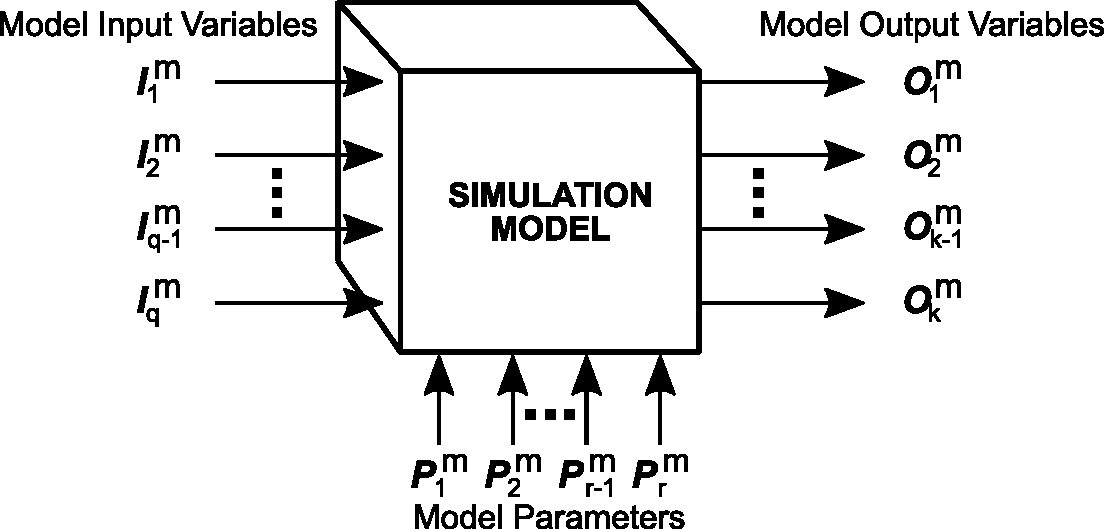
\includegraphics[width=.8\linewidth]{img/schema_parametres_balci.pdf}
	\caption[Les variables d'un modèle de simulation selon \citeauthor{balci_validation_1994}]{Les variables d'un modèle de simulation, adapté depuis \textcite[122]{balci_validation_1994}.\\
	\textit{N.B : ce schéma est tronqué, ne présentant que la partie \og modèle de simulation\fg{} alors que celle-ci est mise en miroir à une partie \og système\fg{} représentant les éléments du domaine empirique.}}
	\label{fig:parametres-Balci} 
\end{figure}

Dans ce schéma et l'article associé, et bien qu'il n'en définisse nulle part explicitement le sens, \citeauthor{balci_validation_1994} esquisse la composition d'un modèle de simulation.
Le modèle est alimenté par des variables en entrée (\textit{Model Input Variables}), qui sont globalement altérées par des paramètres (Model Parameters).
Après passage dans la \og boîte noire\fg{} que représente ici le modèle de simulation ($m$), cela aboutit sur des variables de sortie (\textit{Model Output Variables}).

Notons que si l'auteur du schéma symbolise les entrées, paramètres et sorties au moyen de quatre flèches à chaque fois, leur nombre est variable et sans correspondance.
Il y a ainsi $q$ variables en entrée, $r$ paramètres et $k$ variables en sortie.
Ces nombres différents représentent bien qu'il n'y a pas de lien direct entre les variables en entrée et celles en sortie : la variable en entrée $I_{1}^m$ et la variable en sortie $O_{1}^m$ ne se correspondent pas nécessairement.
De même, \citeauthor{balci_validation_1994} n'indique pas de lien entre les paramètres et les variables (en entrée ou en sortie) : les paramètres agissent à l'échelle du modèle de simulation, sans que les éléments affectés soient précisés.

\paragraph{Paramètres, variables, indicateurs : un essai de définition graphique.}\label{subsubsec:mes_definitions_params}

Dans ce travail de thèse, nous rendons compte de la construction d'un modèle complexe, doté de très nombreux paramètres, variables d'entrée et variables de sortie (selon la définition de \citeauthor{balci_validation_1994}).
Nous avons donc préféré développer notre propre \og ontologie\fg{} de ces termes, qui nous semble plus adaptée à la description d'un modèle tel que SimFeodal.

Comme chez \citeauthor{balci_validation_1994}, notre ontologie est organisée autour d'une opposition entre des \textbf{entrées} et des \textbf{sorties}.

\subparagraph{Les entrées du modèle.}
La \cref{fig:parametres-these-entrees} représente notre proposition de définition des entrées, utilisée dans ce travail de thèse.
Les entrées sont donc composées de deux types d'éléments, des variables et des paramètres.
Les \textbf{variables} ($V_n$) sont des variables informatiques dont la valeur évolue tout au long de la simulation.
Le nombre d'agrégats, par exemple, est une variable : une valeur est assignée à l'initialisation du modèle, et cette valeur est ensuite susceptible de changer à chaque pas de temps.

\begin{figure}[H]
	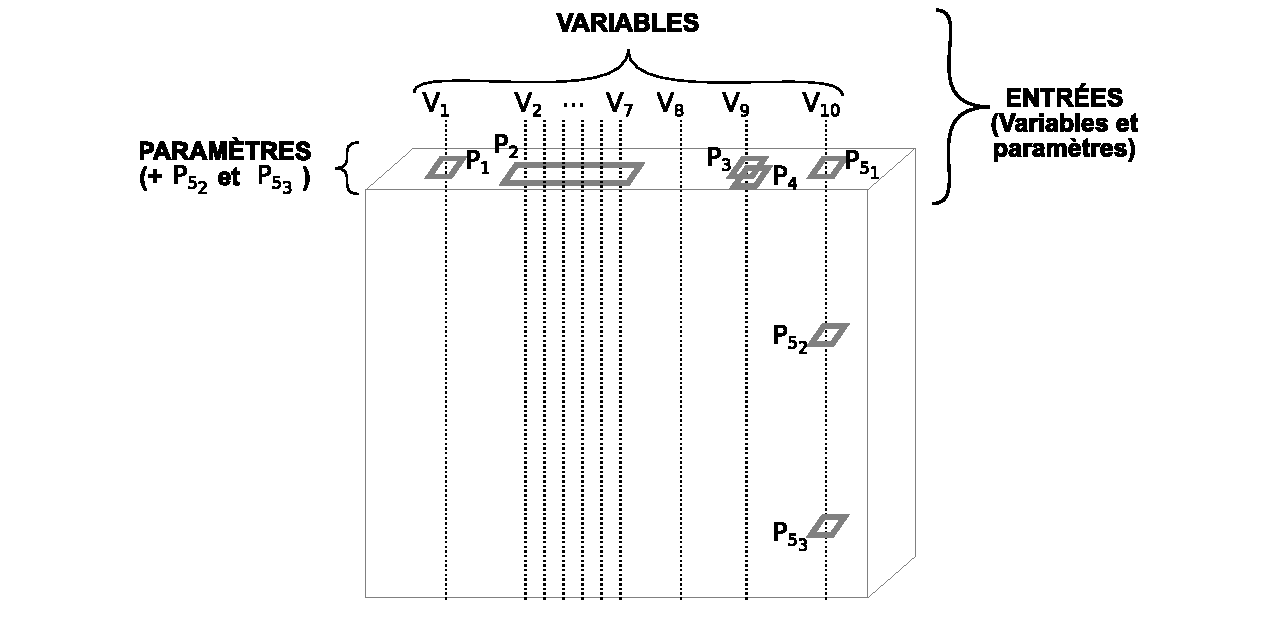
\includegraphics[width=\linewidth]{img/schemas_params_1_entrees.pdf}
	\caption{Les entrées : variables et paramètres.} 
	\label{fig:parametres-these-entrees} 
\end{figure}

Ces variables sont potentiellement affectées par des \textbf{paramètres} ($P_n$), qui peuvent avoir des effets directs sur une unique variable ($P_1$, qui pourrait par exemple représenter le paramètre régulant le nombre d'agrégats à l'initialisation), ou sur plusieurs variables ($P_2$, nombre de foyers paysans par agglomération secondaire antique dans la configuration initiale par exemple).
Plusieurs paramètres peuvent aussi affecter la même variable : dans la figure, la variable $V_9$ est affectée conjointement par les paramètres $P_3$ et $P_4$.
On peut illustrer ce type de cas avec l'exemple du nombre de foyers paysans, qui évoluera en fonction d'une part d'un paramètre définissant la population initiale et d'autre part en fonction d'un second paramètre définissant le taux de croissance.
Le dernier type de paramètre ($P_5$), assez fréquent dans SimFeodal, correspond aux paramètres dont les valeurs peuvent changer au cours de la simulation.
Par exemple, le besoin de protection des foyers paysans évolue au cours du temps simulé, et le paramètre correspondant aura donc plusieurs valeurs, correspondant aux pas de temps où appliquer les différentes modalités prises par le paramètre (voir \cref{sec:inputs}, \hl{chap 2, section 2.6}).
Dans la \cref{fig:parametres-these-entrees}, $P_{5_1}$, $P_{5_2}$ et $P_{5_3}$ correspondent par exemple à l'évolution du seuil de distance acceptable aux châteaux.


\subparagraph{Les sorties du modèle.}
À l'autre bout du modèle, dans la \cref{fig:parametres-these-sorties}, on retrouve encore les variables ($V_n$), dont certaines sont utilisées pour construire des \textbf{indicateurs de sortie} ($I_N$).

\begin{figure}[H]
	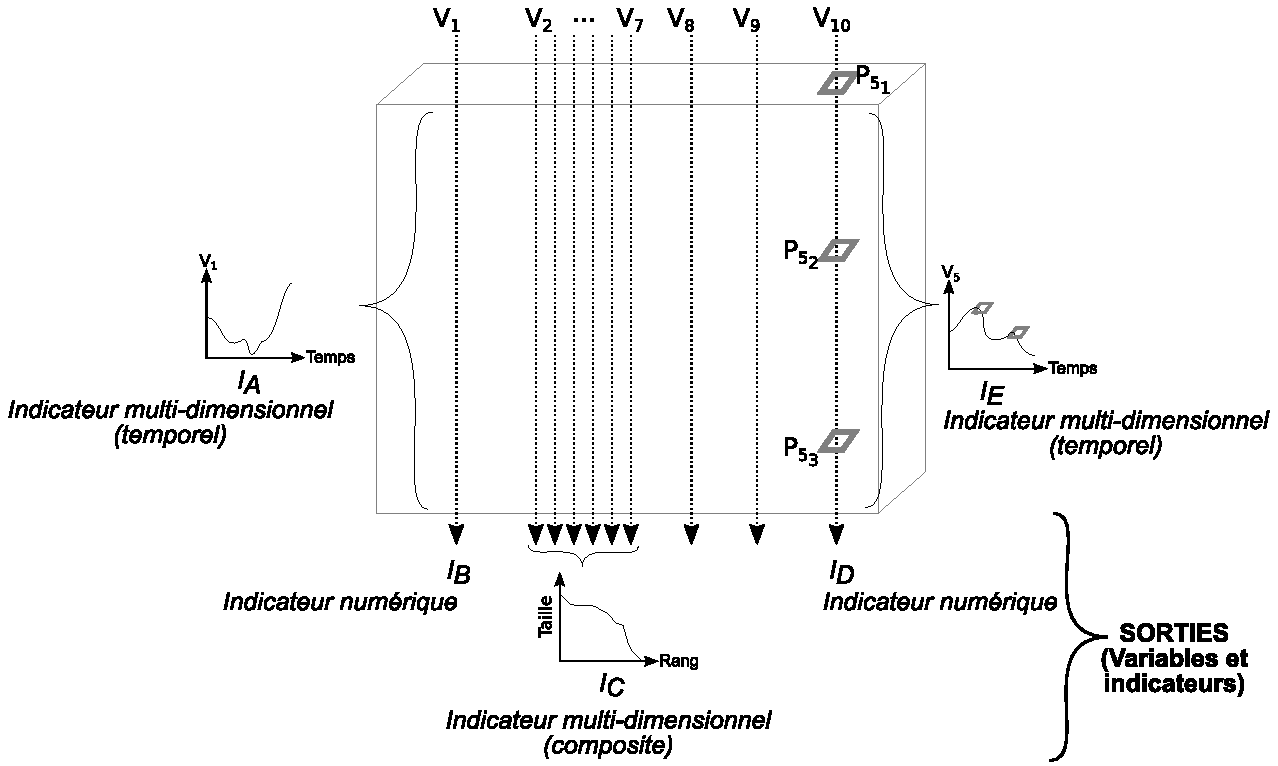
\includegraphics[width=\linewidth]{img/schemas_params_2_sorties.pdf}
	\caption{Les sorties : variables et indicateurs.} 
	\label{fig:parametres-these-sorties} 
\end{figure}

Parmi ces indicateurs de sortie, on identifie là aussi plusieurs types.
Certains indicateurs (ici, c'est le cas de $I_B$ et $I_D$) correspondent directement aux valeurs des variables correspondantes ($V_1$ et $V_{10}$ respectivement) en fin de simulation.
Ces indicateurs sont donc d'une forme numérique (cf. \cref{fig:schema_indices}) simple, et renseignent par exemple sur le nombre de foyers paysans ou d'agrégats de population en fin de simulation.
D'autres indicateurs sont dits \og multi-dimensionnels\fg{} (\cref{fig:schema_indices}) : ils correspondent soit à la combinaison de plusieurs variables en fin de simulation (indicateur $I_C$, qui peut par exemple représenter la courbe rang-taille issue, dans l'exemple de la \cref{fig:parametres-these-sorties}, des variables $V_2$ à $V_7$ qui seraient alors les populations des agrégats), soit à l'évolution temporelle d'une variable (ici ,c'est le cas de $I_A$ et $I_E$).
Ce sont dans ce cas des indicateurs de sortie multi-dimensionnels temporels.
Ceux-ci sont très fortement mobilisés dans l'évaluation de SimFeodal : évolution du nombre d'agrégats, du taux de concentration des foyers paysans, etc.

Notons que si toutes les variables, par définition, varient au cours de la simulation, toutes ne sont pas utilisées pour former des indicateurs de sortie ($V_8$ et $V_9$ dans la figure).
Elles ne sont pas \og inutiles\fg{} pour autant, parce qu'elles peuvent influencer/interagir avec d'autres variables par le biais des mécanismes des agents.
Leur variation aura alors une influence sur d'autres variables, et par conséquent sur différents indicateurs de sortie.

Dans la \cref{fig:parametres-these-sorties}, l'indicateur de sortie $I_E$, de type multi-dimensionnel et temporel, permet de garder à l'esprit que le lien entre variable et paramètre peut être étroit : la variable $V_{10}$, dont la valeur finale est utilisée dans l'indicateur $I_D$, ne peut être étudiée dans son évolution ($I_E$) sans prendre en compte l'influence forte du paramètre évolutif $P_5$.
On retrouve ainsi de fortes inflexions dans l'évolution des valeurs de $V_{10}$ au cours du temps simulé, quand les modalités $P_{5_2}$ et $P_{5_3}$ du paramètre $P_5$ changent.


\subparagraph{Entrées et sorties du modèle.}
La \cref{fig:parametres-these-complet} constitue une synthèse de cette \og ontologie\fg{} lexicale mobilisée dans cette thèse.
Un modèle de simulation comme SimFeodal contient donc en \textbf{entrée} des \textbf{variables}, dont la valeur peut changer au cours du déroulement d'une simulation.
Ces variables peuvent être initialisées ou affectées par des \textbf{paramètres}, qui agissent conjointement et selon des modalités qui peuvent varier au cours du temps.
En fin de simulation, on récupère des \textbf{sorties}, sous la forme d'\textbf{indicateurs de sortie} qui correspondent aux valeurs finales des \textbf{variables}, à leur combinaison, ou encore à leur évolution, temporelle, au cours de la simulation.

\begin{figure}[H]
	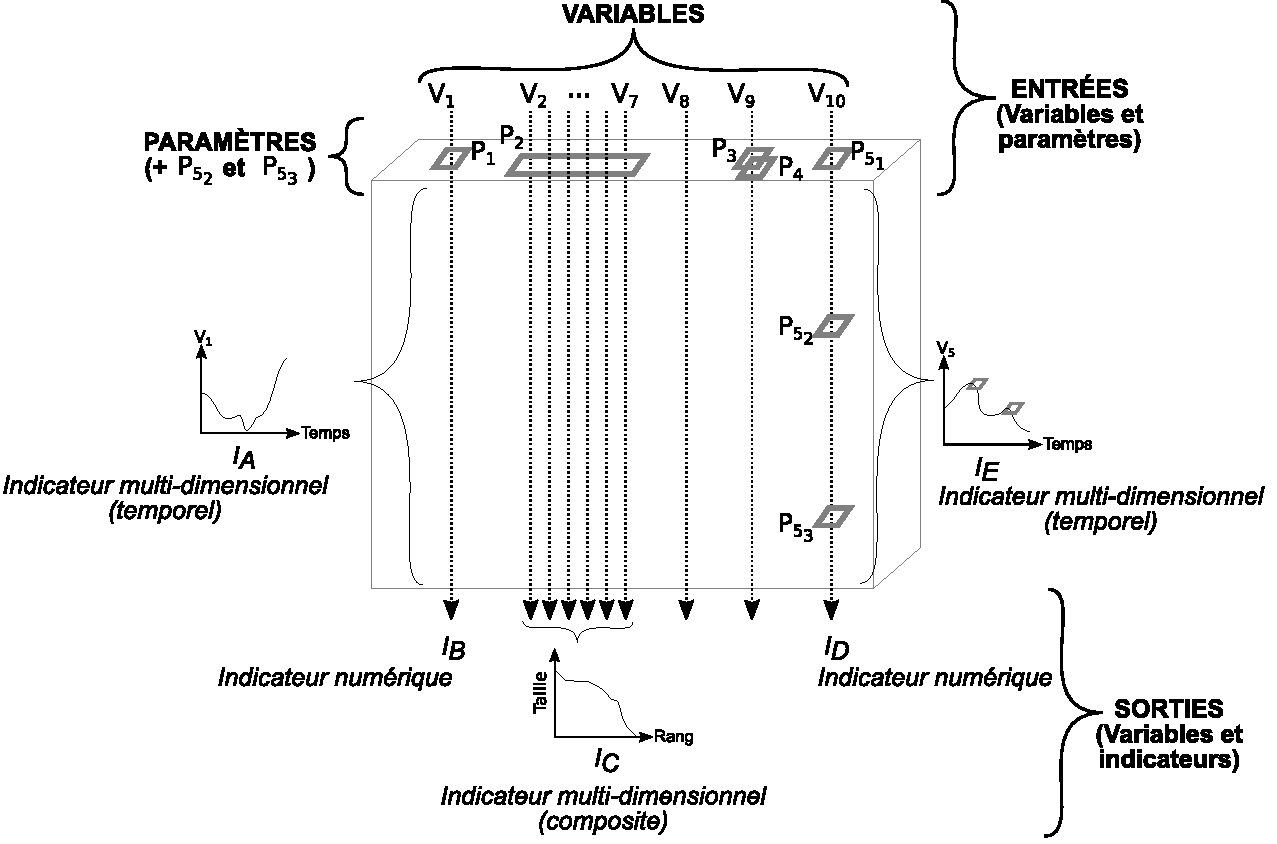
\includegraphics[width=\linewidth]{img/schemas_params_3_complet.pdf}
	\caption{Organisation des entrées et sorties du modèle.} 
	\label{fig:parametres-these-complet} 
\end{figure}

\subparagraph{Paramètres et expériences.}
Les paramètres ont des valeurs pré-définies, par définition, pour l'exécution d'une simulation ou de ses réplications (dans lesquelles les valeurs des paramètres sont volontairement identiques).
Quand bien même leurs modalités peuvent évoluer (c'est le cas de $P_{5_{1}}$, $P_{5_{2}}$ ou $P_{5_{3}}$ dans la \cref{fig:parametres-these-complet}) au cours du temps simulé, c'est un choix effectué avant la simulation et les valeurs et dates d'applications de ces valeurs n'évolueront pas.

Les valeurs des paramètres sont toutefois amenées à évoluer, non pas au sein d'une même simulation, ni même des réplications d'une simulation, mais au sein d'expériences (\cref{fig:parametres-these-experiences}), dont le but est justement de faire varier ces paramètres pour en comparer les effets.
Comme les paramètres varient ($P_2$, $P'_2$ ou $P''_2$ par exemple), il est attendu que les variables de chacune de ces expériences soient affectées différemment.
En faisant varier les paramètres selon les expériences, les indicateurs de sortie tirés de ces variables varieront aussi.
C'est à partir de ces indicateurs de sortie et leurs écarts d'une expérience à l'autre que l'on pourra qualifier les effets des paramètres sur le modèle.

\begin{figure}[H]
	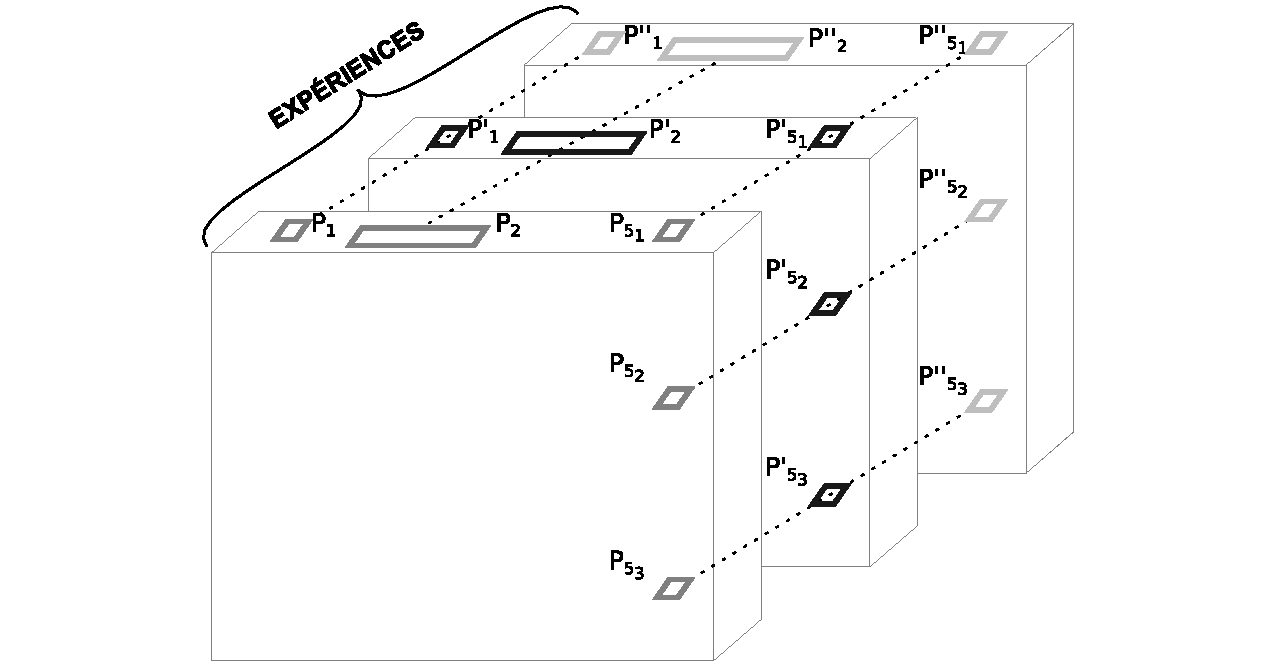
\includegraphics[width=\linewidth]{img/schemas_params_4_experiences.pdf}
	\caption{Variation des paramètres entre les expériences.} 
	\label{fig:parametres-these-experiences} 
\end{figure}


\subsubsection{Les paramètres dans le modèle SimFeodal \label{sssec:types-parametres}}

Les paramètres sont donc un sous-ensemble des entrées d'un modèle qui ont vocation à varier dans les différentes exécutions de ce modèle.
Pour autant, c'est un sous-ensemble assez divers, que ce soit par leur valeur ou par la manière dont ils varient.
Il convient donc d'identifier différents types de paramètres, non selon leur caractéristique propre (c'est-à-dire leurs propriétés, qui permettent de les différencier des sorties par exemple), mais selon leur usage et donc la manière dont on pourra les mobiliser.
À ce titre, la littérature en sciences humaines et sociales
%\footnote{
%	En physique ou en mathématiques par exemple, une telle distinction n'existe pas, la définition d'un paramètre prenant une considération plus simple d'élément rendu constant dans une exécution d'un modèle. \hl{pas clair, prendre une définition quelconque reprenant cette idée.}
%}
distingue souvent deux types de paramètres.
D'un côté, des paramètres empiriques, dont la valeur a une correspondance directe dans le domaine empirique (on peut donc l'observer), et d'un autre, les paramètres techniques\footnote{
		\textcite{mathian_formalisation_2015} utilisent le terme de paramètre mécanique pour définir ce type de paramètres.
		Nous trouvons l'usage du mot \og technique\fg{} plus approprié, en ce qu'il se différencie plus de l'empirique sur le pan de l'usage qui en est fait et que le terme de \og mécanique\fg{} peut rappeler celui de mécanisme, alors même que les paramètres, empiriques ou non, ont une implication pour les mécanismes.
}, pour lesquels cette correspondance n'existe pas.
Comme dans la plupart des typologies ayant trait à la catégorisation de valeurs numériques, de nombreux paramètres peuvent se trouver à l'interface de ces deux classes.
Comme les paramètres de SimFeodal sont nombreux (\hl{voir l'annexe N, tableau de tous les paramètres}) et seraient trop sommairement distingués dans ces deux catégories, nous avons choisi de mobiliser une typologie en quatre classes (voir \cref{enc:types-parametres}), relatives au sens de ces paramètres vis-à-vis du fonctionnement du modèle.
Cette typologie est mixte, entre d'une part le degré de connaissance empirique sur lequel chaque paramètre repose (paramètres techniques \textit{vs} les autres), et d'autre part l'usage qui en est fait dans le modèle (\textit{input} et contexte \textit{vs} les autres).
Cette typologie est notamment appuyée sur celle de \textcite[45]{tannier_analyse_2017}.

\begin{encadre}{Quatre types de paramètres}{types-parametres}
\renewcommand{\thempfootnote}{\alph{mpfootnote}}

Dans SimFeodal, nous avons choisi de différencier les paramètres en quatre \og types\fg{}, qui distinguent l'usage	qui est fait de chacun de ces paramètres dans le modèle, en particulier vis-à-vis des connaissances expertes sur lesquelles ils reposent ou non.\vspace*{-1em}
	
\subparagraph*{Paramètres d'\textit{input}.}
	Ce sont les paramètres qui définissent l'état du monde simulé lors de son initialisation.
	Ils sont fortement basés sur les connaissances empiriques, liés à la région qui est modélisée (la Touraine).
	À ce titre, ces paramètres d'\textit{input} ne sont donc pas amenés à varier en dehors d'application du modèle à d'autres cas d'étude, ou si de nouvelles connaissances empiriques viennent les modifier.\\
	\textit{Exemples : nombre de seigneurs, de villages, d'églises, etc. à l'initialisation, dimensions du monde modélisé\ldots}\vspace*{-1em}

\subparagraph*{Paramètres de contexte.}
	Les paramètres de contexte ont un ancrage empirique moins appuyé, mais agissent de manière globale et continuelle sur le contexte de déroulement du modèle.
	Ce sont les paramètres sur lesquels on peut s'appuyer majoritairement pour l'exploration des hypothèses thématiques du modèle.
	Leurs variations entre des expériences différentes est nécessairement guidée par l'empirie.\\
	\textit{Exemples : taux de croissance démographique, puissance des communautés, période de construction des châteaux\ldots}\vspace*{-1em}	

\subparagraph*{Paramètres de mécanisme.}
	Ces paramètres ont une assise empirique plus incertaine, s'appuyant plus sur des ordres de grandeur que les précédents.
	Ils agissent au niveau des mécanismes des agents, et peuvent varier, tout en restant dans les mêmes ordres de grandeur, lors du paramétrage du modèle.\\
	\textit{Exemples : seuils de distances aux églises et châteaux pour les foyers paysans, probabilité de dons de zones de prélèvement et de châteaux pour les seigneurs, attractivité relative des attracteurs qui composent les pôles\ldots}\vspace*{-1em}

\subparagraph*{Paramètres techniques}
	Il s'agit des paramètres dont les valeurs, ou même les ordres de grandeur, ne s'inscrivent sur aucune connaissance empirique.
	Ces paramètres ont pour raison d'être de permettre à d'autres types de paramètres de s'exprimer en valeurs compréhensibles et exploitables.
	Dès lors, leurs valeurs sont propres à chaque version, sous-version ou expérience du modèle formalisé, et une comparaison de ces valeurs entre les différentes versions d'un modèle n'apporte pas de connaissance.
	Ils sont amenés à varier d'une manière uniquement guidée par l'évaluation du modèle lors du paramétrage, sans que cela ait le moindre ancrage ou répercussion empirique.\\
	\textit{Exemples : distance de fusion entre les agrégats, pondération de la satisfaction matérielle des foyers paysans en fonction du nombre de droits acquittés, montants récupérés par les seigneurs selon les types de droits\ldots}
\end{encadre}

Avec cette typologie des paramètres basée non sur la nature de ceux-ci mais sur leur utilisation dans le modèle, nous nous inscrivons dans une vision fonctionnaliste et donc très subjective, rappelant la définition d'un modèle de \citeauthor{minsky_matter_1965}.
Selon l'usage que l'on fait du modèle, un même paramètre pourra donc être vu comme un paramètre de contexte ou de mécanisme (par exemple selon l'état des connaissances empiriques liées à ce paramètre sur le cas d'étude traité).

\paragraph*{Comment choisir les valeurs de paramètres ?}


Après avoir présenté notre définition des paramètres, nous pouvons désormais revenir sur le processus qui les mobilise et a demandé cette explicitation : le paramétrage.

Cette étape, que nous allons maintenant définir et illustrer, consiste ainsi notamment à \og ajuster\fg{} les valeurs des paramètres, ou plus exactement de certains des paramètres, en se basant notamment sur la typologie mise en place dans ces pages (paramètres d'\textit{input}, de contexte, de mécanisme, techniques).

\subsection{Le paramétrage}

Le paramétrage d'un modèle est souvent réduit à l'un de ses aspects, le \og calibrage \fg, étape finale de la construction d'un modèle qui cherchera à reproduire autant que possible un ensemble de données observées dans le domaine empirique en faisant varier les valeurs des paramètres jusqu'à ce qu'une combinaison de celles-ci soit satisfaisante.

Le plus souvent, une fois le modèle construit, le modélisateur s'attache à son \og calibrage\fg{}, en cherchant pour chaque paramètre la ou les valeurs qui permettront au modèle de s'approcher, au plus près, des données empiriques devant être reproduites, c'est-à-dire la conjugaison de \og valeurs optimales\fg{} de paramètres minimisant l'écart entre les données simulées et les données empiriques de contrôle.
Cette étape, que l'on nomme aussi souvent calibration par anglicisme, peut se faire de manière manuelle, par approximations successives, et on parle alors de  méthode \og essais-erreurs\fg{} (\textit{trial-and-error}), par exemple chez des auteurs tels que \textcite{batty_spatial_1973}\footnote{
	Les auteurs définissent ainsi cette méthode : \og
	The trial and error method of calibration involves running the model under different parameter values which are fixed systematically within some predetermined range.
	The performance of the model is assessed during each run and the range is gradually narrowed as the search homes in on what appears to be the best level of performance\fg{} \autocite[356]{batty_spatial_1973}.
	Notons que récemment, certains auteurs ont utilisé la dénomination de \og calibration qualitative\fg{} pour définir cette approche \autocite[253]{crooks_agent-based_2019}.
}.
Le calibrage peut aussi être effectué de manière semi-automatique, par exemple en effectuant des analyses de sensibilité.
\textcite[\S2.3--2.4]{thiele_facilitating_2014} mobilisent ainsi l'analyse de sensibilité, via échantillonnage, pour faire de l'estimation de paramètres.
Enfin, il est possible de mener le calibrage de manière entièrement automatique, souvent à l'aide de méthodes mathématiques d'optimisation.
\textcite{heppenstall_genetic_2007} et \textcite[188]{ngo_calibration_2012}, par exemple, effectuent le calibrage de leurs modèles à l'aide de d'une famille de méthodes informatiques nommées \og algorithmes génétiques\fg{}.

De nombreux auteurs ont montré que le paramétrage d'un modèle ne pouvait se réduire à cette étape, chacun employant des termes différents pour désigner le processus de paramétrage, processus le plus souvent inscrit comme l'une des composantes de l'évaluation des modèles (chez \textcite{ngo_calibration_2012}, cf. \cref{fig:schema_ngo} par exemple).

Dans notre travail, nous souhaitons revenir sur cette approche de la modélisation, ancrant le paramétrage comme étape ultime de la construction d'un modèle, en particulier en ce que nous considérons que cette pratique de recherches de valeurs optimales est un exercice qui devrait s'effectuer tout au long de la construction du modèle, de manière plus itérative que conclusive.

\subsubsection{Définition \label{sssec:definition-parametrage}}

Le terme de paramétrage recouvre deux sens différents, dont la distinction peut se faire selon qu'on l'utilise pour définir un processus ou pour caractériser une configuration.
Ici, nous emploierons plutôt le premier cas, définissant dès lors le paramétrage comme le processus, manuel ou automatique, visant à constituer une configuration optimale de paramètres.
Dans ce deuxième cas, le paramétrage désigne un ensemble de valeurs de paramètres, par exemple dans l'expression \og paramétrage par défaut\fg{}, ou un paramétrage optimal.
Pour ne pas risquer de contre-sens, nous réserverons le terme de paramétrage au processus, et nous utiliserons l'expression de \og jeu de valeurs de paramètres\fg{} pour désigner la seconde acceptation.

Le terme de paramétrage est très employé dans la littérature, le plus souvent comme un synonyme \og faible\fg{} de calibrage, c'est-à-dire sans l'aspect quantifié et \og final\fg{} que ce dernier terme contient.
Nous choisissons ici de nous distinguer de ces approches, en différenciant calibrage et paramétrage.
Dans un premier temps, cependant, il nous paraît important de re-situer le paramétrage (et le calibrage), en les incluant dans la construction du modèle plutôt que dans son évaluation, au contraire donc de l'approche de  \textcite{klugl_validation_2008} et \textcite{ngo_calibration_2012} visible dans les \cref{fig:schema_kluegl,fig:schema_evaludationl}.

Le paramétrage est en effet une pratique utile dans la construction du modèle, car les résultats auxquels il aboutit, c'est-à-dire les valeurs de paramètres qui semblent les mieux adaptées, renseignent aussi bien sur les biais des mécanismes adoptés que sur leur efficacité réelle.
Par exemple, quand, après avoir ajouté un mécanisme, on se rend compte que des variations dans les valeurs de paramètres ne changent pas réellement les sorties du modèle, cela peut être l'occasion de repenser le mécanisme dans son ensemble, ou plus souvent, la manière dont le paramètre est mobilisé dans ce mécanisme.
On retrouve cette logique dans l'exploration par Clara Schmitt du modèle SimpopLocal \autocite{schmitt_modelisation_2014}, qui a permis de réaliser que la variation de l'un des paramètres ($InnovationLife$) n'avait que peu d'impact sur les sorties du modèle, tout en rendant son calibrage plus complexe et instable :
\begin{quotation}
\noindent\og
	Au-dessous du seuil des 150 pas de simulation pour le paramétrage de InnovationLife, le calibrage du modèle est très difficile voire impossible.
	Au-dessus de ce seuil, le mécanisme associé au paramètre InnovationLife n'a plus d'effet sur le calibrage du modèle.
	Dans un souci de parcimonie du nombre et de la complexité des mécanismes simulés dans le modèle SimpopLocal, il est justifiable de retirer du modèle ce mécanisme qui n'est pas nécessaire à la simulation de la dynamique de croissance recherchée.
	\fg{}\\
	\mbox{}~ \hfill \textcite[224]{schmitt_modelisation_2014}
\end{quotation}


Dans ce travail de thèse, nous reprenons ainsi le sens du terme paramétrage tel qu'initialement employé par \textcite{hirtzel2015exploration}\footnote{
	\og
	La notion de paramétrage d'un modèle est souvent associée à celle de calibrage, et ces deux notions, bien que différentes, sont parfois confondues dans la littérature (Richiardi et al., 2006).
	Le calibrage consiste à tester plusieurs jeux de paramètres possibles pour une variable et à choisir l'un d'eux pour l'exécution des simulations, selon sa capacité à atteindre les objectifs définis.
	Il constitue ainsi une étape du paramétrage d'un modèle.
	Cette étape n'est pas forcément indispensable : si les valeurs initialement affectées permettent d'atteindre les objectifs du modélisateur, celui-ci n'a pas besoin de procéder à un calibrage.\fg{} \autocite[136]{hirtzel2015exploration}.
} et ensuite explicité par \textcite{tannier_analyse_2017} :
\begin{quotation}
\noindent \og 
Le paramétrage d'un modèle consiste à fixer les valeurs des variables et paramètres de mécanisme, au moyen d'analyses spatiales ou statistiques de données empiriques, de transcriptions de dires d'experts, ou de simulations avec le modèle.
Le paramétrage comprend une phase d'estimation (statistique ou autre) des valeurs des paramètres et variables, et une phase de calibrage si celle-ci est nécessaire.
\fg{}\\
\mbox{}~ \hfill \textcite[52]{tannier_analyse_2017}
\end{quotation}

Nous ne retiendrons pas dans ce travail la notion de phase d'estimation, mais trouvons nécessaire d'ajouter à cette définition une composante d'implémentation qui consiste à adapter l'implémentation des mécanismes de manière à en rendre le résultat plus satisfaisant.
Cela n'implique pas de changer le modèle conceptuel, et n'est pas non plus véritablement un changement dans l'implémentation du modèle.
Par exemple, changer l'ordonnancement du détail d'un mécanisme relève à notre sens du paramétrage.

On peut illustrer cela avec l'exemple du mécanisme de définition du contour spatial des agrégats (cf. \hl{méca, 2.7.2.1, chap2}): un \textit{buffer} est actuellement appliqué autour de l'enveloppe convexe formée par les foyers paysans membres d'un agrégat afin de fusionner d'éventuels agrégats très proches.
On peut adapter ce mécanisme en appliquant ce \textit{buffer} à la fin du mécanisme plutôt qu'au milieu, une fois que l'héritage des agrégats précédents a été transféré par exemple.

Cela n'aurait pas un impact important sur le plan conceptuel, ni même d'ailleurs lors de l'observation agrégée de tous les agrégats.
Toutefois, au niveau local, cela peut avoir un impact non négligeable sur l'historique des agrégats.
À notre sens, il s'agit d'une adaptation du modèle du même ordre qu'un changement de valeur de paramètre, et nous incluons ainsi ce type de modifications dans le processus de paramétrage.


\paragraph{Les étapes du processus de modélisation.}

De nombreux termes sont utilisés dans la littérature, souvent sans réelle distinction, pour désigner cette opération qui consister à choisir un jeu de paramètres pour un modèle.
Pêle-mêle, on y retrouve le paramétrage, le calibrage, l'ajustement, l'estimation, etc.
Nous proposons une représentation graphique, dans la \cref{fig:etapes-modelisation}, de notre usage du sous-ensemble de ces termes mobilisé dans cette thèse, et en donnons des définitions dans l'\cref{enc:termes-calibration}.

\begin{figure}[H]
	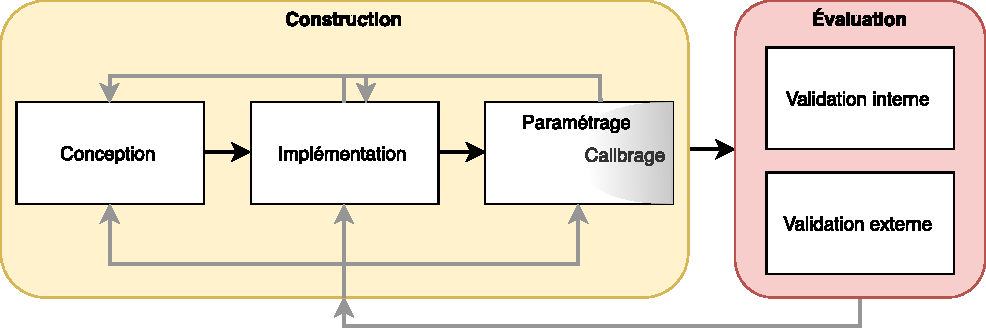
\includegraphics[width=1\textwidth]{img/schema_definition_parametrage.pdf}
	\caption{Étapes du processus de modélisation.} 
	\label{fig:etapes-modelisation} 
\end{figure}


\begin{encadre}{Construction, paramétrage et calibrage}{termes-calibration}
\renewcommand{\thempfootnote}{\alph{mpfootnote}}
	
La \cref{fig:etapes-modelisation} représente l'enchevêtrement des différentes étapes du processus de modélisation, dont nous allons brièvement détailler les parties relatives à la construction ici.
	
\subparagraph{Construction.}
Par construction, nous définissons l'ensemble des étapes relatives à la création du modèle, c'est-à-dire la conception du modèle conceptuel, son implémentation sous forme d'un modèle de simulation et le paramétrage du modèle.
À force d'allers-retours entre ses composantes, la construction aboutit à un modèle \og finalisé\fg{}, qui peut être évalué de manière globale (chacune des composantes de la construction pouvant être évaluée individuellement : l'implémentation est par exemple évaluée au moyen des méthodes de validation interne).\\
\textit{N.B. : Le terme de co-construction est d'un niveau de généricité supérieur à celui de la construction ici définie.
La co-construction, définie dans le \hl{chapitre 1}, désigne l'approche mise en place lors de chacune des étapes du modèle, et s'applique donc aussi bien à la construction qu'à l'évaluation.}
		
\subparagraph{Paramétrage.}
Le paramétrage du modèle est l'étape où l'on adapte le modèle après avoir vérifié sa cohérence vis-à-vis des éléments empiriques qu'il cherche à reproduire.
Lors du paramétrage, on ajuste les valeurs de paramètres, leur utilisation par les mécanismes et le détail du fonctionnement technique de ces mécanismes.
On cherche à obtenir un modèle plus satisfaisant du point de vue des dynamiques et résultats qu'il produit.
Une des définitions du nouveau petit Robert \autocite{robert_nouveau_1993} nous semble particulièrement représentative de cela :\\
\og Paramétrer (informatique): \og Programmer (un appareil complexe), en définissant les paramètres assurant son fonctionnement optimal.
Ex. \textit{Paramétrer une imprimante}\fg{}.
		
\subparagraph{Calibrage.}
On réserve souvent, et nous nous y tiendrons, ce terme à la dernière étape dans l'aboutissement d'un modèle.
Une fois les mécanismes fixés et des objectifs définis, on peut procéder au calibrage (aussi nommé, par anglicisme, \og calibration\fg{}), c'est-à-dire à une exploration de l'espace des paramètres ayant pour but de stabiliser les paramètres afin de se rapprocher autant que possible des objectifs.
Dans cette thèse, nous inscrivons le calibrage comme une des étapes, finale, du paramétrage.

\medskip
\noindent Notons que toutes ces étapes sont représentées de manière linéaire et chronologique, le paramétrage marquant la fin de la construction du modèle et l'évaluation la fin de l'\og{}évolution\fg{} du modèle.
Pour autant, les allers-retours entre ces étapes sont extrêmement nombreux (flèches grises), et la \cref{fig:etapes-modelisation} aurait aussi pu être représentée (en perdant en simplicité) sous forme d'une spirale, voire d'une hélice, comme la \og vis sans fin\fg{} d'Archimède.

\end{encadre}

\subsubsection{Paramétrer des modèles, illustrations}
Afin d'illustrer ces propos, on peut s'appuyer sur des modèles bien connus de la littérature, issus de deux champs disciplinaires différents : le modèle gravitaire (\cref{enc:param-gravitaire}) et le modèle de Schelling (\cref{enc:param-schelling}).


\begin{encadre}{Paramétrage du modèle gravitaire}{param-gravitaire}
	\renewcommand{\thempfootnote}{\alph{mpfootnote}}
\subparagraph{Description.}
Ce modèle, formalisé mathématiquement,
%\footnote{
%	Pour une description plus complète, se référer à l'ouvrage de \textcite{pumain_les_2001}.
%}
, dans la formulation qu'en a faite \textcite{stewart_demographic_1948}, vise à prédire des flux ($F_ij$) potentiels (démographiques, marchands, etc.) entre des lieux à partir d'une analogie avec la loi physique de la gravitation.
Dans le formalisme le plus simple, \og sans contrainte\fg{} \autocite{pumain_les_2001}, on peut l'exprimer ainsi :
\begin{equation*}
F_{ij} = \frac{k \times M_{i} \times M_{j}}{d_{ij}{}^\alpha}
\end{equation*}

Le modèle comprend deux paramètres ($k$ et $\alpha$).
$k$ est un paramètre technique (\cref{enc:types-parametres}), ses fluctuations ne donnent aucune information supplémentaire sur le système étudié.
$\alpha$ est un paramètre de contexte : il est basé sur une logique empirique, et conditionne fortement le modèle (et notamment les valeurs du paramètre $k$).
En faisant varier $\alpha$, on explore des hypothèses thématiques relatives à l'importance de la distance dans l'intensité des interactions entre les composantes du système modélisé.

À partir des variables empiriques $M_i$ et $M_j$ qui caractérisent les masses (populations, ou stocks de  marchandise par exemple) des lieux $i$ et $j$, et de la distance qui les sépare $d_{ij}$, on peut ainsi prédire $F_{ij}$, le potentiel d'interaction entre ces lieux.

\subparagraph{Objectif.}
Afin que ce modèle donne des ordres de grandeur réalistes quant aux quantités échangées, il faut le paramétrer en définissant une valeur de $k$, permettant dès lors d'obtenir un rapport entre les masses d'origine et les quantités échangées.
La valeur de ce paramètre est conditionnée par celle de $\alpha$, que l'on nomme fréquemment \og frein de la distance\fg{}, en ce qu'il permet de quantifier l'impact qu'aura un éloignement plus ou moins important sur la quantité de flux échangés.

\subparagraph{Paramétrage.}
Pour \og ajuster\fg{}\footnote{
	C'est le terme employé par \textcite{pumain_les_2001}, que l'on peut ici retenir comme équivalent de paramétrer.
	\textcite[298]{durand1995modeles} utilise pour sa part le terme de calibration à propos du même modèle.
} le modèle, il faut donc en réaliser le paramétrage en s'appuyant sur les éléments connus de l'équation (les valeurs empiriques).
$\alpha$ et $k$ étant liés dans l'équation, la valeur de chacun de ces paramètres dépend de celle choisie pour l'autre, et un changement dans l'un des paramètres entraînera la nécessité de modifier l'autre.

La technique la plus simple pour paramétrer le modèle consiste à réaliser une régression linéaire sur les logarithmes décimaux des distances et des flux observés, $k$ prenant alors la valeur du logarithme de l'ordonnée à l'origine et $\alpha$ celle du coefficient directeur de la courbe.	
Le modèle est alors calibré (voir \cref{enc:termes-calibration}).
Si on souhaite donner une valeur spécifique à l'un des paramètres, par exemple pour utiliser une valeur classique de 2 au frein de la distance ($\alpha$) \autocite{pumain_modegravitaire_2004}, il faudra alors le re-soumettre au paramétrage pour adapter $k$.
De même si l'on modifie les lieux et/ou les masses sur lesquels il s'applique.
\end{encadre}

La manière classique de mener le paramétrage du modèle gravitaire est donc directe et déterministe.
Pour une configuration donnée de masses et de distributions spatiales -- impliquant les distances --, un et un seul jeu de valeurs de paramètres permet un ajustement optimal, c'est-à-dire d'assurer un écart minimal entre les valeurs empiriques et les valeurs théoriques (simulées).
Le paramétrage de ce modèle se résume donc à l'étape de calibrage.


\begin{encadre}{Paramétrage du modèle de ségrégation de Schelling}{param-schelling}
\renewcommand{\thempfootnote}{\alph{mpfootnote}}

\subparagraph{Description.}
Le modèle de Schelling\footnote{
	Une description plus poussée accompagnée d'une description de l'exploration du modèle peut être lue dans \autocite{daude_comparaison_2006}
} est un modèle de simulation décrit par l'économiste \textcite{schelling_dynamic_1971} qui vise à montrer comment un espace peut passer d'un état correspondant à une répartition aléatoire, potentiellement intégrée, à un état ségrégé ethniquement à travers une succession de comportements individuels de mobilité résidentielle.
Il montre en particulier qu'on peut parvenir à un état ségrégé même quand les comportements individuels sont majoritairement tolérants à la présence d'individus d'un autre groupe.

L'espace du modèle est défini comme une grille carrée composée de $N$\footnote{
	Nous reprenons ici la notation $M(N, d, n, S)$ proposée par \textcite[433]{daude_comparaison_2006} en n'explicitant toutefois pas le paramètre $n$ décrivant le type de voisinage (4 ou 8) utilisé.
} cellules.
Au début de la simulation, des agents de deux types, en proportions similaires, sont distribués aléatoirement dans l'espace du modèle.
Chaque agent occupe une cellule, et le nombre total de cellules occupées (et donc d'agents) dépend d'un paramètre de densité $d$ qui représente la part (entre $0\%$ et $100\%$) du nombre de cellules qui sera occupée.
Chaque agent est défini par une satisfaction, fonction du voisinage des agents.
Ce voisinage correspond à la part de cellules voisines occupées par des agents \og étrangers\fg{}, c'est-à-dire d'un autre type : plus le voisinage contient d'étrangers, moins l'agent est satisfait.
Si cette satisfaction est inférieure à un paramètre de tolérance $S$, qui représente un seuil à ne pas dépasser, l'agent est considéré comme insatisfait et se déplace aléatoirement dans une cellule non occupée.
À terme, Schelling montre que même en considérant des valeurs de $S$ assez élevées, c'est-à-dire un comportement plutôt tolérant, la succession de choix individuels entraîne la mise en place d'une distribution spatiale très ségrégée.
On considère que le modèle a convergé quand l'ensemble des agents sont satisfaits, ce que ne permettent pas toutes les combinaisons de valeurs de paramètres.

Dans ce modèle, on peut donc identifier trois paramètres, $N$, $S$ et $d$.
$N$ peut être vu comme un paramètre d'\textit{input}, en ce qu'il définit une partie de la configuration spatiale, mais aussi comme un paramètre technique.
Il n'y a en effet aucune correspondance entre l'espace empirique modélisé et
sa représentation théorique dans le modèle de simulation.
$S$ est un paramètre de contexte : il a un ancrage empirique, certes limité, mais dont l'ordre de grandeur peut être estimé par des sociologues ou psychologues.
De plus, c'est le paramètre qui conditionne thématiquement la convergence ou non du modèle vers un état stable.
C'est donc le paramètre qui sera mobilisé pour tester les hypothèses, empiriques ou théoriques, des modélisateurs.
Le dernier paramètre, $d$, peut être vu comme un paramètre technique puisqu'il ne s'appuie sur aucune connaissance empirique, mais aussi comme un paramètre de mécanisme : il n'a de sens que parce que le mécanisme de déplacement des agents dirige ceux-ci vers un \og espace vide\fg{}, et agit donc comme un paramètre de régulation de ce mécanisme.
Avec un modèle conceptuel très proche, où les agents seraient capables \og d'échanger\fg{} leur position plutôt que de rejoindre une cellule non occupée, ce paramètre n'aurait pas de sens.

\subparagraph{Objectif.}
Le paramétrage de ce modèle consiste à fixer un $N$ constant et à faire varier $d$ et $S$ afin de trouver des valeurs permettant la convergence vers une situation stable.
Quand $d$ est très faible ($30$\% dans l'exemple de \textcite{daude_comparaison_2006}), quelles que soient les valeurs de $S$, le modèle converge rapidement :
	quand l'espace du modèle dispose d'une faible densité d'agents, il est facile pour ceux-là de créer des agrégats homogènes distants d'agrégats de l'autre type d'agents.
Quand $d$ est plus important ($\geq66$\%), l'espace disponible étant limité, toutes les valeurs de $S$ ne permettent pas la convergence du modèle.
Le paramétrage du modèle aura donc pour objectif de trouver la valeur maximale possible -- pour un $N$ et un $d$ donné -- que peut prendre le paramètre de tolérance $S$ tout en laissant le modèle converger.

\subparagraph{Paramétrage.}
Contrairement au modèle gravitaire, le modèle de Schelling est stochastique.
Les agents se déplacent en effet de manière aléatoire quand ils ne sont pas satisfaits.
Dès lors, deux exécutions du modèle avec le même jeu de paramètres n'entraîneront pas forcément la même configuration spatiale.
Qui plus est, pour certains jeux de paramètres, seules certaines exécutions convergeront.
Le paramétrage de ce modèle ressemble donc à celui qui est réalisé pour le modèle SimFeodal.
La manière \og traditionnelle\fg{}, c'est-à-dire manuelle et basée sur une méthode d'essais-erreurs, consiste à fixer un $d$, puis à essayer d'augmenter le $S$ tant que le modèle converge.
Si le modèle converge pour tout $S$, on augmente la valeur de $d$ et on recommence à chercher la valeur maximale possible pour $S$.
De part la nature stochastique du modèle, chaque jeu de paramètres doit être simulé plusieurs fois, le nombre de ces réplications dépendant de la part d'aléa dans le comportement du modèle.
Un modèle de Schelling calibré, c'est-à-dire dont le paramétrage est achevé,
donnera pour un $N$ fixé les valeurs maximales de $d$ et de $S$ atteignables.
\end{encadre}

Le paramétrage du modèle de Schelling est donc très différent de celui du modèle gravitaire.
Pour ce dernier, il s'agit d'un calcul résultant d'une estimation statistique, alors que dans le cas du modèle de Schelling, on mobilise l'approche d'essais-erreurs.
Cette approche nous semble plus représentative de la démarche classique de paramétrage des modèles de simulation à base d'agents.
Contrairement au modèle gravitaire, le paramétrage est ainsi exécuté de manière itérative et répétée : à chaque augmentation de la valeur de $d$, il faut ré-exécuter le calibrage du paramètre $S$, voire de $N$ si on choisit de faire varier ce paramètre aussi.


À travers ces deux exemples ayant traits à des méthodes différentes, on retrouve deux approches de paramétrage que l'on souhaite ici voire confondues :
	dans le premier cas, le paramétrage du modèle gravitaire tend à son calibrage, à la recherche d'une solution optimale, c'est-à-dire meilleure que toute autre.
Pour un phénomène donné (un jeu de données précis par exemple) et un formalisme donné (l'expression la plus simple du modèle, ici sans contrainte), seul un couple de paramètres $\alpha$ et $k$ permet ainsi d'obtenir des flux modélisés proches des flux observés.
Dans le cas du modèle de Schelling, il n'y a pas de recherche d'optimum.
On ne cherche en effet pas à reproduire, terme à terme, une répartition observée de deux populations.
Le paramétrage permet de comprendre le modèle en en définissant les limites en matière de convergence.
Une configuration de paramètres $S$ et $d$ ne sera pas meilleure qu'une autre, mais pour un $S$ donné, on saura quelle est la valeur maximale de $d$ permettant de parvenir, le plus souvent (en tenant compte de l'aléa) à cette convergence (et réciproquement).

\subsubsection{Paramétrer SimFeodal}

\paragraph{Que ou quand paramétrer ?} \label{sssec:parametrer-un-des-modeles}

Ce dernier exemple montre l'importance des allers-retours entre évaluation et paramétrage, et illustre la démarche itérative et incrémentale du paramétrage.
Parmi les étapes du paramétrage, le calibrage devrait ainsi être mené à chaque \og version\fg{} du modèle.
Ces versions, dans le modèle de Schelling, pourraient correspondre à un changement de valeur de $N$ ou de $d$, qui définissent le contexte du modèle.
Quand ces paramètres évoluent, il est ainsi nécessaire d'évaluer le modèle qui en résulte (y a-t-il convergence ?), et en fonction du résultat, de calibrer les autres paramètres de manière à obtenir une configuration optimale.

Sans aller jusqu'à voir dans ces versions successives des modèles à part entière -- ce que les tenant de la modélisation modulaire \autocite{grimm_pattern-oriented_2005,grimm_pattern-oriented_2012} ou multi-modélisation \autocite{pumain_chapter_2017} peuvent laisser entendre --, on peut tout de même considérer que chacune de ces versions requiert des cycles de construction et d'évaluations indépendants les uns des autres (cf. \cref{fig:etapes-modelisation}).
Chacune de ces versions devra dès lors être adaptée par un paramétrage dédié.

C'est, à notre sens, d'autant plus important que certaines versions de modèles peuvent donner lieu à des évolutions majeures, conceptuelles, méthodologiques ou techniques.
Le paramétrage est dans ce cas à \og re-faire\fg{} entièrement, c'est-à-dire que les étapes précédentes de paramétrages ne peuvent plus forcément aider à réduire l'amplitude des valeurs parmi lesquels fixer les paramètres par exemple.

Pour illustrer ce propos, on peut prendre l'exemple d'une modification qui a eu lieu sur SimFeodal au cours de son développement (dans la version \og 0\fg{}, cf. \cref{tab:historique-versions-simfeodal}).
On considérait jusque-là que pour prendre en compte la population rurale (hors Tours donc), une population de 1 000 foyers paysans correspondant à une estimation probable de la situation en 800 de l'espace considéré.
Lors d'une réunion, les thématiciens ont ré-évalué ce nombre, remarquant d'après d'autres connaissances expertes qu'il sous-estimait très largement la population réelle.
En menant de nouvelles estimations, ils ont conclu que le nombre de foyers paysans devait finalement être fixé à 4 000, et que le paramètre dédié devait ainsi être ajusté à cette valeur.

Les autres paramètres, fixés en bonne partie empiriquement, n'avaient \textit{a priori} aucune raison d'évoluer du fait de ce changement.
Les mécanismes  et effets de seuil étaient en effet conçus de manière à être relatifs aux masses manipulées, et le changement attendu était une augmentation linéaire des indicateurs de sortie.

Dans les faits, cette légère modification a cependant entraîné une obligation de repenser la quasi-totalité des autres paramètres et d'ajuster une bonne part des mécanismes, de la même manière qu'un changement de $N$ dans le modèle de Schelling (\cref{enc:param-schelling}) demande de revoir $d$ et $S$.

La concentration des foyers paysans était en effet bien trop rapide par un effet mécanique dû au nombre plus important d'individus, et donc à une densité accrue.
Le modèle convergeait en quelques pas de temps vers une configuration presque statique et très concentrée.
Tous les mécanismes de régulation de ce comportement étaient dès lors rendus ineptes, et il a fallu changer en profondeur la manière dont chaque paramètre et mécanisme interagissait avec les autres.

On peut illustrer les effets de ce changement de valeur de paramètre en analysant, de manière visuelle, l'évolution du modèle qui en a suivi.
Une étude des \og \textit{commits}\fg{} de SimFeodal a été menée à cet effet.
Les \textit{commits} sont des enregistrements de l'état d'un ensemble de fichiers, et contiennent en tant que telle la liste des changements apportés depuis l'enregistrement (\textit{commit}) précédent.
Les \textit{commits} peuvent contenir plusieurs modifications : un même \textit{commit} peut porter sur le changements de plusieurs valeurs de paramètres par exemple.
Les \textit{commits} peuvent aussi contenir des modifications situées dans plusieurs fichiers différents.
Comme le modèle SimFeodal est composé d'une dizaine de fichiers correspondant entre autre aux différents types d'agents, les \textit{commits} concernent souvent plusieurs fichiers : le changement de mécanisme d'un type d'agent sera souvent matérialisé dans le fichier de l'agent correspondant, dans le fichier gérant les \textit{outputs} du modèle, et par exemple dans le fichier régulant l'ordonnancement des mécanismes.

Ici, on a catégorisé, manuellement, les \textit{commits} des premières versions de SimFeodal selon les modifications conceptuelles apportées : ajout de mécanisme, modification de valeurs de paramètres ou autre (nouvelles expériences, documentation, débuggage, nettoyage de code, etc.)
Un même \textit{commit} peut contenir plusieurs ajouts de mécanismes, et/ou plusieurs modifications de valeurs de paramètres, et/ou encore plusieurs autres changements dans le code-source du modèle.
Dans la \cref{fig:comits-periodes}, on a représenté ces \textit{commits} selon la part de modifications relatives à chacune de ces catégories : une barre 100\% noire signifie que le \textit{commit} n'a porté que sur de l'ajout de mécanisme, une barre 50\% noire et 50\% grise correspond à un \textit{commit} qui a autant porté sur l'ajout de mécanisme que sur la modification de valeurs de paramètres, et une absence de barre indique un \textit{commit} dont tous les changements relèvent de la catégorie \og autre\fg{}.

\begin{figure}[H]
	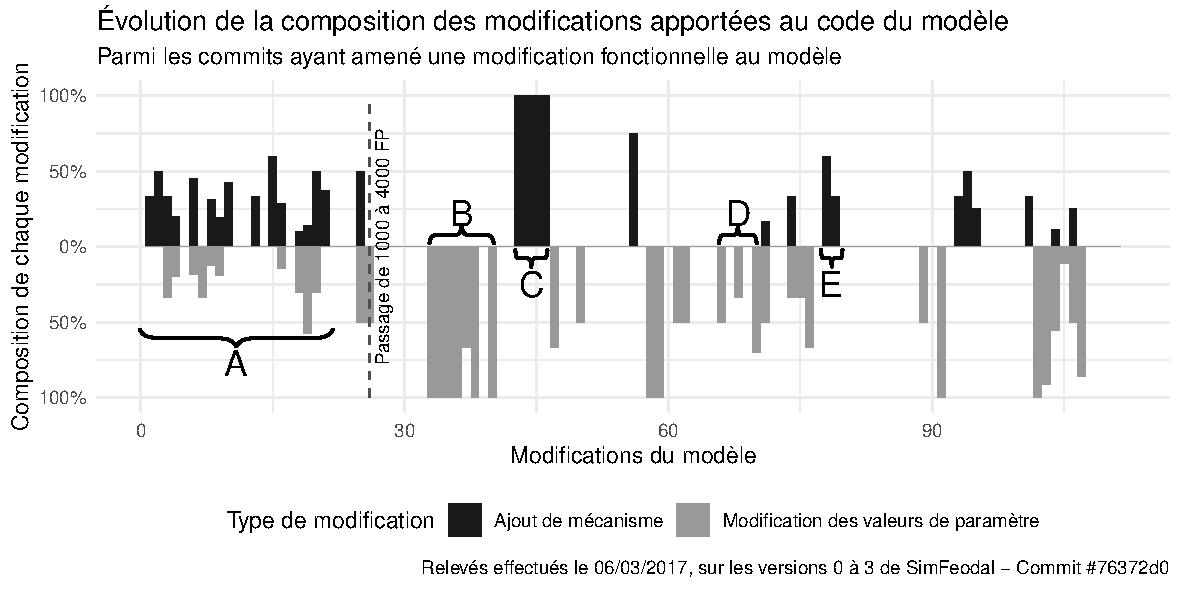
\includegraphics[width = \linewidth]{img/plotComits_clean.pdf}
	\caption[Temporalité du paramétrage du modèle.]{Temporalité du paramétrage du modèle.}
	\label{fig:comits-periodes}
\end{figure}

La \cref{fig:comits-periodes} permet de constater un changement majeur suite à la modification du nombre de foyers paysans, entre les périodes \textbf{A} et \textbf{B} de l'évolution du modèle.
Après le passage de 1000 à 4000 foyers paysans, suit ainsi une période intense de changements de valeurs de paramètres (\textbf{B}).
C'est une phase de calibrage, où l'on essaye d'ajuster les valeurs de chaque paramètre de manière à obtenir des résultats satisfaisants en sortie de simulation, résultats qui ont été bouleversés par le changement du nombre initial de foyers paysans.

L'étape \textbf{C} montre une succession d'ajouts et de changements dans les mécanismes : le calibrage des paramètres n'a pas été suffisant pour que le modèle produise une situation acceptable.
Le calibrage ne suffisant pas, on revient en effet à d'autres phases de paramétrages, en modifiant les mécanismes de manière itérative.
Entre les étapes \textbf{C} et \textbf{D}, on note quelques modifications de paramètres, quelques ajouts de mécanismes, et de nombreux \textit{commits} catégorisés comme \og autre\fg{} (il n'y a pas de barre) : cela correspond à des modifications plus substantielles dans le modèle.

L'enchainement des étapes \textbf{D} et \textbf{E} ressemblent à celui de \textbf{B} et \textbf{C} : on recommence ainsi un cycle de calibrage-paramétrage-changements d'implémentation de manière à améliorer le modèle de manière itérative, selon le principe classique de l'essai-erreur.
En catégorisant l'ensemble des \textit{commits} du modèle jusqu'à la dernière version en date, nous sommes convaincus que ce motif réapparaîtrait de manière fréquente et régulière.

Cet exemple, construit sur l'évolution effective de SimFeodal, illustre le caractère nécessaire du paramétrage, et qui plus est, montre que ce processus doit être mené de manière continue et répétée.
Dans un modèle exploratoire comme SimFeodal (\hl{cf. chap1 ou chap2}), le paramétrage ne peut pas être considéré comme une étape ultime, restreinte au calibrage, qui donnerait lieu à validation du modèle.
Un paramétrage répété, régulier, donnant lieu à des évaluations systématiques, est ainsi la seule manière de garantir la comparabilité des différentes versions et sous-versions successives d'un modèle.
Dans le cas contraire, on court le risque de disqualifier une version du modèle qui aurait pu être plus plausible que les suivantes mais n'a pas été ajustée comme elle aurait pu l'être.

\paragraph{Quels paramètres ?} \label{sssec:quels-parametres}

Dans la partie précédente, nous avons distingué plusieurs types de paramètres (voir l'\cref{enc:types-parametres} dans la \cref{sssec:types-parametres}), selon leur usage dans le modèle et leur niveau d'inscription dans les connaissances empiriques.
Cette distinction nous semble particulièrement utile pour dresser une hiérarchie des paramètres sur lesquels jouer pour ajuster le modèle.

Les \textbf{paramètres d'\textit{input}}, pour commencer, n'ont pas vocation à changer lors de l'évolution du modèle : ils ont été définis de manière empirique, et ne peuvent donc revêtir d'autres valeurs uniquement pour améliorer l'ajustement du modèle.
Toutefois, si les connaissances expertes évoluent, les phases de paramétrage du modèle sont l'occasion de répercuter ces nouvelles connaissances.
Les changements de ces paramètres peuvent résulter d'un besoin de préciser la mise en œuvre des connaissances empiriques\footnote{
	Un exemple d'un tel choix est présenté dans le \hl{chapitre 6} (\hl{partie 6.1.1.1}), où l'on a choisi de faire passer les dimensions du monde simulé de 100×100 km à 80×80 km.
}, ou simplement de la correction d'approximations inexactes\footnote{
	Comme c'est le cas dans l'exemple du passage de 1000 à 4000 foyers paysans présenté plus haut.
}.
Dans tous les cas, le paramétrage de ces paramètres n'est pas guidé directement par les résultats d'une version du modèle, mais par les connaissances qui y sont injectées.
Il en va de même pour les \textbf{paramètres de contexte} : ils peuvent être précisés ou corrigés, mais leur paramétrage ne doit pas être guidé par l'évaluation du modèle.

Les \textbf{paramètres techniques} sont des candidats naturels au paramétrage, et plus spécifiquement à sa composante de calibrage.
Puisqu'ils ne reposent sur aucune connaissance empirique, ils constituent ainsi des \og leviers\fg{} sur lesquels on pourra mener le paramétrage, y compris de manière automatisée pour ces paramètres dont on peut faire varier les valeurs de plusieurs ordres de grandeur sans conséquence conceptuelle ou empirique sur le modèle.
Le paramétrage des paramètres techniques est aisé mais n'apporte rien, d'un point de vue heuristique, en termes de connaissances supplémentaires sur le modèle où sur ce qui est modélisé.
Ces paramètres sont toutefois très \og pratiques\fg{} pour compenser le paramétrage des autres types de parmètres, comme dans l'exemple du modèle gravitaire (\cref{enc:param-gravitaire}).
Si de nouvelles connaissances viennent pousser à modifier un paramètre de contexte par exemple (comme le paramètre de frein de la distance $\alpha$), on peut espérer parvenir à compenser cette variation, sur les sorties, en modifiant un paramètre technique ($k$ dans le modèle gravitaire) en conséquence.

Le cas des \textbf{paramètres de mécanisme} est plus emblématique du processus de paramétrage : ils reposent sur des ordres de grandeur plus incertains, et leur valeur peut donc assez librement être modifiée.
Lors du paramétrage, il faut naturellement s'assurer de ne pas les faire varier en dehors des intervalles définis empiriquement, mais ils se prêtent très bien à des ajustements manuels.
On peut ainsi sans crainte procéder à des modifications successives, par allers-retours entre l'évaluation des sorties du modèle et le changement de valeur de ces paramètres.
On pourra de cette manière figer, temporairement -- en attendant de nouveaux ajustements dus au paramétrage d'autres paramètres --, des valeurs dont l'effet combiné sera plus satisfaisant sur le déroulement et l'aboutissement des simulations.

Rappelons aussi, comme indiqué lors de la définition (\cref{sssec:definition-parametrage}), qu'en dehors des valeurs des paramètres, le paramétrage est aussi l'occasion de modifier, d'une manière modérée, le détail de l'implémentation de certains mécanismes.

\paragraph{Historique de SimFeodal.}\label{par:historique-versions-simfeodal}

Tout au long de cette thèse, nous avons souvent mentionné les versions et sous-versions de SimFeodal.
Il nous paraît important ici de les exposer (\cref{tab:historique-versions-simfeodal}) ainsi que de décrire la logique de leur distinction.

\begin{table}[H]
\centering
\resizebox{1.2\textwidth}{!}{%
{\renewcommand{\arraystretch}{1.2}%
\begin{tabular}{|M{1.6cm}|M{2.25cm}|M{1.7cm}|M{2cm}|M{1.7cm}|M{7cm}|}
\hline
\textbf{Version} & \textbf{Date} & \textbf{Nom original} & \textbf{Nombre de sous-versions} & \textbf{Nombre de \textit{commits}} & \textbf{Changements principaux} \\ \hline
0 & 21/04/2014 & Base & ---\footnotemark[1] & 168 & ---\footnotemark[2] \\ \hline
2 & 13/04/2016 & Base2 & 3 & 31 &
\begin{itemize}[before=\vspace{.5em},after=\vspace{-1em},leftmargin=*]
	\item Mise en place d'une hiérarchie des attracteurs
	\item Ajout de la création de paroisses urbaines
	\item Ajout de la différenciation entre châteaux et gros châteaux
\end{itemize} \\ \hline
3 & 28/08/2016 & Base3 & 4 & 39 & \begin{itemize}[before=\vspace{.5em},after=\vspace{-1em},leftmargin=*]
	\item Réduction des distances de déplacement local
	\item Modification du mécanisme de construction de châteaux
	\item Modification de la logique de calcul de la satisfaction matérielle
\end{itemize} \\ \hline
4 & 25/04/2017 & Base4 & 7 & 59 & \begin{itemize}[before=\vspace{.5em},after=\vspace{-1em},leftmargin=*]
	\item Changement de la répartition initiale des foyers paysans
	\item Changement du mécanisme d’héritage/reconnaissance des agrégats
	\item Changement du mécanisme de définition des pôles
\end{itemize} \\ \hline
5 & 11/06/2018 & v5 & 4 & 60 & \begin{itemize}[before=\vspace{.5em},after=\vspace{-1em},leftmargin=*]
	\item Modification générale de l'ordonnancement des mécanismes
	\item Modification du mécanisme de définition des agrégats
	\item Modification du calcul de satisfaction des foyers paysans
	\item Mise en place de seuils évolutifs pour le déplacement local
\end{itemize} \\ \hline
6 & 09/01/2019 & v6 & \makecell{6 \\ \footnotesize{(22/09/2019)}} & 63 & \begin{itemize}[before=\vspace{.5em},after=\vspace{-1em},leftmargin=*]
	\item Renommage global et refactorisation des paramètres
	\item Suppression des mécanismes de lignage seigneurial
	\item Changement du mécanisme de répartition des nouveaux châteaux
	\item Changement des calculs de probabilité de construction de châteaux
\end{itemize} \\ \hline
\end{tabular}}
}
\caption{Historique des versions de SimFeodal.}
\label{tab:historique-versions-simfeodal}
\end{table}
\footnotetext[1]{Si le code était bien historisé à l'époque, la logique de versionnement n'était pas encore véritablement à l'œuvre.}
\footnotetext[2]{Cette version 0 est marquée par une forte instabilité et par de très fréquents changements.
	On notera d'ailleurs qu'il n'y a pas de version 1.
	En effet, si la version 0 est la première version \og complète\fg{} du modèle, c'est la version 2 qui est la première a avoir été un tant soit peu satisfaisante du point de vue de l'évaluation.}

À partir de la version \og 2\fg{} de SimFeodal nous avons partiellement suivi les règles de \og versionnement sémantique\fg{} (ou \og SemVer\fg{}\footnote{
	\og \textit{Semantic versioning}\fg{}, voir \href{https://semver.org/}{https://semver.org/}.
}), c'est-à-dire la numérotation des versions selon une logique de \og VersionMajeure.SousVersion.Patch\fg{}.

On différencie ainsi des versions selon leur rétro-compatibilité, notamment au niveau de leurs sorties : entre la version 5 et la version 6 de SimFeodal, on retrouve de très nombreuses modifications du code (paramètres, mécanismes, sorties) qui sont organisées selon des versions 5.0, 5.0.1, 5.1, 5.1.1, etc.
Le modèle passe à la version 6 quand les paramètres sont renommés et que les données en sortie ne sont donc plus directement organisées de la même manière qu'auparavant.
Il y a alors rupture dans la rétro-compatibilité, et on passe de la version 5.1.2 à la version 6.0.

Au sein de chaque version, on retrouve plusieurs sous-versions (appelées \og versions mineures\fg{} dans le modèle de versionnement SemVer), qui apportent toutes des changements suffisants pour justifier un changement de version (évolution de plusieurs paramètres et/ou mécanismes), mais dont la compatibilité avec les versions précédentes est totale.

Au sein de ces sous-versions, on peut encore distinguer des \og sous-sous-versions\fg{} (\og \textit{patchs}\fg{} en SemVer), qui concernent cette fois des modifications plus restreintes.
Dans l'évolution de SimFeodal par exemple, les sous-sous-versions correspondent à différents essais de changement de paramètres qui s'inscrivent dans la démarche d'essais-erreurs définie auparavant.
Ces sous-sous-versions ne constituent donc pas nécessairement une étape supplémentaire dans l'évolution \og linéaire\fg{} du modèle : les sous-sous-versions 5.0.1 et 5.0.2 sont concurrentes et correspondent à des essais.
L'itération suivante du modèle (la version 5.1 par exemple) pourra s'appuyer sur n'importe laquelle de ces sous-sous-versions, par exemple la 5.0.1 plutôt que la 5.0.2.

Au niveau de la granularité la plus fine enfin, chaque version, sous-version et sous-sous-version est composée de \og \textit{commits}\fg{}, c'est-à-dire d'enregistrements historisés du code du modèle à un instant \textit{t}.
Ces \textit{commits} contiennent un intitulé qui renseigne sur le contenu des modifications apportées, et surtout, ils intègrent une liste précise de ces modifications : les modifications de chaque ligne (de chaque fichier) modifiée sont ainsi conservées.
Souvent, les \textit{commits} de SimFeodal \footnote{
	Il y en a plus de 400 à l'approche du rendu de ce travail, consultables dans le dépôt logiciel de SimFeodal :\\
	\faGithub~ \href{https://github.com/SimFeodal/SimFeodal/commits/master}{https://github.com/SimFeodal/SimFeodal/commits/master}
} sont \og atomiques\fg{}, c'est-à-dire qu'ils ne contiennent et ne documentent qu'un seul changement : paramètre modifié, modification d'un mécanisme, ajout d'une expérience\ldots
Cette atomicité n'est pourtant pas constante, et un \textit{commit} peut contenir des centaines de modifications aussi bien qu'une seule.

Cette forte hétérogénéité des \textit{commits} met en évidence un dernier point qui nous paraît important.
L'énumération menée dans cette thèse des versions, des sous-version ou encore de tout changement du modèles, est exprimée selon un ordre chronologique, organisé au sein de la hiérarchie des versions, sous-versions et patchs.
Pour autant, comme indiqué dans le \hl{chapitre 1}, la réalité de la construction d'un modèle, qui plus est dans un contexte exploratoire et collectif, ne peut s'inscrire nettement dans cette linéarité et dans cet emboitement de versions.
Le paramétrage et la construction d'un modèle, et du nôtre en particulier, représentent en effet un travail constant d'allers-retours entre l'identification et la résolution de problèmes.
Par conséquent, la structure réelle de développement, que l'on peut retrouver dans l'historique des modifications du modèle (les \og \textit{commits}\fg{}), ne correspond donc pas exactement à la chronologie reconstruite visible dans le \cref{tab:historique-versions-simfeodal}.
De la même manière que la version 5.1 pouvait être basée sur la 5.0.1 plutôt que que la 5.0.2, la version 6.3 peut correspondre à une amélioration de la version 6.1, sans ré-utilisation de ce qui avait été modifié en 6.2.

\paragraph{Exploration de l'évolution d'un modèle exploratoire.}

Afin d'appuyer notre discours relatif à la nécessité de mener l'évaluation et le paramétrage de manière continuelle et systématique, il nous a semblé approprié d'illustrer ce discours autour de l'analyse \textit{a posteriori} de l'évolution d'un modèle de simulation.
Le cas de SimFeodal, modèle exploratoire, nous semble tout à fait convenir à une telle analyse exploratoire.

Le travail de qualification de chaque modification du modèle réalisé pour la \cref{fig:comits-periodes} était difficilement extensible à l'ensemble des \textit{commits} de SimFeodal\footnote{
	La \cref{fig:comits-periodes} résulte de la classification manuelle d'une centaine de \textit{commits}.
	Pour chacun, il a été nécessaire d'en regarder le contenu a posteriori, de vérifier les mécanismes affectés, les paramètres ajoutés, modifiés, renommés, etc.
	A la date de la version 6.5 du modèle, l'historique de versionnement est composé de plus de 400 commits, et il aurait donc été nécessaire de reproduire ce travail méticuleux et coûteux en temps sur plus de 300 \textit{commits} supplémentaires.
}.
Il nous cependant semblé intéressant et innovant, de mener une analyse exploratoire, moins détaillée (sans catégoriser manuellement chaque \textit{commit}) mais plus étendue, de l'évolution du modèle SimFeodal sur la durée complète, de plus de 5 ans, de son cycle de co-construction.

Pour mener cette analyse, nous avons analysé de manière automatique chacun des \textit{commits} de SimFeodal, en observant, pour chacun, le nombre de lignes de code qui avaient été modifiées.
Un changement d'une ligne de code, par exemple, correspond souvent à la modification de la valeur d'un paramètre, alors que la modification d'un mécanisme entraîne le changement d'une dizaine à une cinquantaine de lignes.
Pour ne pas biaiser l'analyse avec les changements de la documentation du modèle, ou encore avec les fichiers relatifs à l'exécution d'expériences, nous n'avons conservé que les changements de code effectués dans les fichiers relatifs au cœur du modèle.

Le \textit{commit} est une l'unité \og atomique\fg{} du versionnement, mais n'est pas nécessairement homogène pour autant, comme indiqué précédemment.
A ce titre, il arrive souvent qu'un \textit{commit} soit suivi rapidement après d'un second, voir d'un troisième \textit{commit} venant en corriger un tout petit aspect (faute de syntaxe dans le code, oubli de répercussion d'une modification dans les sorties\ldots).
Nous avons donc aussi agrégé ces \textit{commits} à l'échelle de la journée, en considérant que les commits d'une même journée de travail formaient un ensemble cohérent.
On aurait aussi pu agréger les commits sur une période plus longue, par exemple de deux ou trois jours.
Cela correspond dans les faits plus souvent au temps réel d'implémentation ou de test d'une changement dans le modèle.
Cette durée représente cependant aussi celle des sessions de travail collectif avec l'ensemble des concepteurs de SimFeodal, sessions pendant lesquelles l'activité est plus intense et le nombre de changements et d'allers-retours aussi.
L'agrégation à la journée nous a ainsi semblé la moins biaisée.
C'est un raccourci assez important, sans doute peu adapté pour de nombreux \textit{commits}, mais cela nous paraît utile d'une part pour diminuer le nombre d'éléments à analyser, et d'autre part pour diminuer la part des \textit{commits} négligeables correspondant aux oublis et corrections décrits auparavant.

On a ensuite caractérisé le contenu de ces agrégations de \textit{commits} journaliers en mesurant la taille médiane (en nombre de lignes de code modifiées) et la somme de ces modifications pour chaque jour (total des nombres de lignes de codes modifiées).
La \cref{fig:methodo-agreg-commits} présente un exemple de ces agrégations.

\begin{figure}[H]
	\centering
	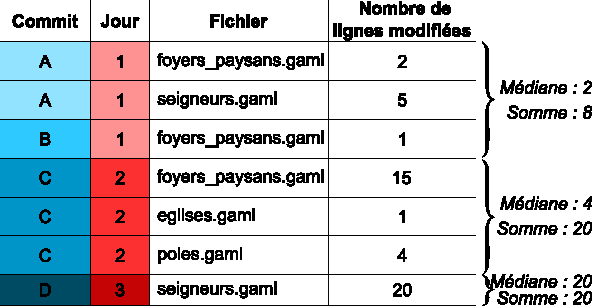
\includegraphics[width=.75\linewidth]{img/tableau_exemple_commits.pdf}
	\caption[Méthodologie d'agrégation des \textit{commits}.]{Méthodologie d'agrégation des \textit{commits}.}
	\label{fig:methodo-agreg-commits}
\end{figure}

La somme des modifications étant par nature d'un ordre de grandeur bien plus élevé que la médiane\footnote{
	Le changement médian maximal représente un changement de 300 lignes de codes, alors que la somme concerne, elle, plus de 1500 lignes\ldots
}, on a normalisé (réduction sans centrage) les valeurs afin qu'elles soient comparables graphiquement.
La \cref{fig:explo-edits-code} est une représentation de cette analyse\footnote{
	Dans cette figure, les modifications regroupées dans l'accolade \og B\&C\fg{} correspondent aux phases B et C identifiées dans la  \cref{fig:comits-periodes}.
}, qui permet de visualiser le \og rythme\fg{} des changements de SimFeodal et d'en tirer quelques remarques.


\begin{figure}[H]
	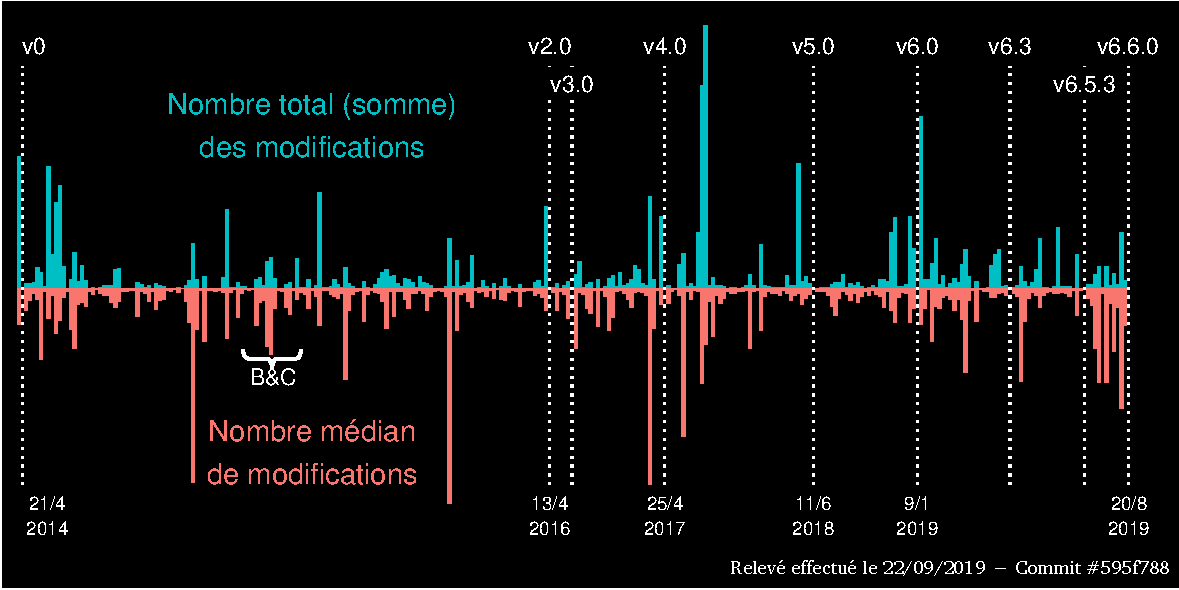
\includegraphics[width=1\linewidth]{img/explo_edits_code_clean.pdf}
	\caption[Une exploration visuelle du rythme des changements de SimFeodal.]{Une exploration visuelle du rythme des changements de SimFeodal.\\
		\textit{N.B. : L'axe des abscisses n'est pas linéaire du point de vue temporel : l'ordre chronologique y est respecté, mais le temps n'y est pas régulier.}
	}
	\label{fig:explo-edits-code}
\end{figure}

On y remarque en premier lieu un certain motif, qui pourrait presque s'apparenter aux pulsations cardiaques, où l'on note des changements majeurs, espacés, entre lesquels de plus faibles phases de modifications surviennent.
Ce \og rythme\fg{} est avant tout une scorie de la manière dont le modèle a évolué, autour des versions représentées sur le graphique.

Les phases de plus intenses modifications, concrétisées ou précédées par des changements de version, sont ainsi intimement liées au rythme de ce travail de co-construction interdisciplinaire : les pics marquent en général la préparation, l'exécution, et les résultats immédiats des séances de travail collectives.
Ces réunions étaient ainsi l'occasion d'évaluer le modèle, que ce soit en analysant ses sorties (évaluation externe) ou en ré-exposant les choix d'implémentation (évaluation interne), et en conséquence d'en mener le paramétrage, en faisant évoluer les paramètres et mécanismes.
Certains pics correspondent aussi à des moments de production de \og livrables\fg{}, que ce soit à l'occasion de publications ou de communications, où il fallait stabiliser le modèle pour en communiquer les résultats.

À un niveau d'observation plus fin, on peut noter, aussi bien sur la somme des modifications que sur leur médiane, que les pics principaux sont le plus souvent précédés par une augmentation de la taille et de la quantité totale de modifications, puis suivis d'une diminution de ces deux indicateurs.
Sur le plan \og temporel\fg{}, cela correspond aux phases de préparation des réunions, faite de petites explorations locales du comportement du modèle en vu de l'adapter, puis aux phases collectives résultant sur des choix de modifications plus importantes, modifications ensuite ajustées et finalement validées, jusqu'à la réunion suivante.
Cette figure donne ainsi à voir un aperçu concret du processus de co-construction qui a été privilégié dans notre groupe de travail.

Sur le plan conceptuel, cela correspond à différentes phases de construction du modèle : les modifications qui précèdent les changements de version sont d'abord assez modérées, en médiane comme en somme.
Cela correspond à du paramétrage assez modéré, portant sur la modification marginale de quelques valeurs de paramètres.
À mesure que la taille des \textit{commits} augmente, ces modifications sont de plus en plus importantes, et consistent ainsi à l'ajustement de plus de paramètres, à la modification plus fréquente de détails de mécanismes, etc.

Les changements de version résultent le plus souvent d'une insatisfaction vis-à-vis de l'aboutissement de ces phases de paramétrage : même en poussant le paramétrage, même en menant un calibrage approfondi on ne parvient pas à obtenir des résultats de simulation assez satisfaisants.
Il est alors nécessaire de revenir sur le modèle conceptuel et son implémentation (flèches grises de la \cref{fig:etapes-modelisation}), et donc de mener des modifications plus conséquentes, par exemple en transformant véritablement le fonctionnement de certains mécanismes.
Les mécanismes étant modifiés, avec ajout ou suppression de paramètres par exemple, la rétro-compatibilité des sorties du modèle n'est plus assurée\footnote{
	Sans même considérer d'ajout/suppression de paramètre, les modifications du sens et de l'utilisation effective de certains paramètres peuvent rendre leurs valeurs non comparables avec celles des versions précédentes.
}, et l'on change alors de version.

Après ces changements de version, la taille des modifications diminue, jusqu'à atteindre des niveaux très faibles : la somme des modifications devient négligeable (à mi-chemin entre les versions 4 et 5 dans la \cref{fig:explo-edits-code} par exemple)  et la médiane des \textit{commits} est elle aussi très faible.
Cela correspond exactement aux phases de paramétrages qui suivent les changements majeurs : le nombre de changements diminue, jusqu'à aboutir à des modifications difficilement discernables qui correspondent au calibrage.
Dans cette étape, seules une ou deux lignes de code changent en général, ce qui correspond aux modifications d'une valeur de paramètre.

On retrouve donc dans cette figure, et dans l'évolution effective de SimFeodal, l'ensemble des étapes décrites dans ce chapitre.
Des phases de construction et d'évaluation se succèdent, avec à chaque fois un travail de paramétrage, parfois suivi de nouvelles phases d'implémentation voire de conception.
On notera aussi que les versions sont assez visibles sur ce graphique, correspondant aux pics principaux, de même que les sous-versions, où les pics sont plus modérés : entre la version 6 et la fin du graphique (version 6.6), on arrive même sans difficulté à identifier chacune des sous-versions intermédiaires (6.1, 6.2\ldots).

\paragraph{Aboutissement du paramétrage.}

Avec cette analyse exploratoire et l'exercice d'interprétation qui l'accompagne, nous avons voulu illustrer d'une part le processus de paramétrage mis en œuvre dans le modèle SimFeodal, mais surtout, d'autre part appuyer notre proposition de démarche de co-construction de modèles.
Qui plus est dans un contexte interdisciplinaire, l'évolution du modèle ne peut ainsi passer que par des allers-retours fréquents entre son évaluation et sa modification.

\section*{Conclusion}
\label{sec:chap3-conclu}
\addcontentsline{toc}{section}{Conclusion}

Le paramétrage, et notamment sa composante de calibrage, ne peuvent être réduit à un exercice ultime et unique, qui viserai à \og finaliser\fg{} un modèle avant son emploi.
Au contraire, l'application fréquente et régulière de phases d'évaluation et de paramétrage permet de garantir que les différentes pistes de modélisation explorées sont bien comparables, car justement comparées sur des versions aussi finement ajustées que possible à chaque fois.

Dans ce chapitre, nous avons présenté et proposé une approche originale pour mener ces phases d'évaluation d'un modèle de simulation à base d'agents.
Cette approche, que nous nommons évaluation visuelle, nous paraît très adaptée à l'évaluation de modèles exploratoires construits dans un contexte interdisciplinaire.
L'évaluation visuelle propose une évaluation basée sur la multiplication des points de vue, au moyen de nombreux indicateurs de sortie.
Nous pensons en effet que l'apport des différents acteurs de la modélisation, chacun avec son expertise thématique propre, permet une évaluation approfondie d'un modèle et que cette étape participe pleinement de la dimension heuristique de la modélisation.
La mise en place d'une grille d'évaluation, \textit{a priori}, et la hiérarchisation des critères permet de plus de garantir une vision globale de la capacité d'un modèle à produire et faire émerger les faits stylisés que l'on cherche à modéliser au sein d'une approche générative.

La forte profusion et diversité des indicateurs de sortie identifiés constitue de plus une aide précieuse au paramétrage d'un modèle : en multipliant les perspectives d'analyse des sorties d'un modèle, on facilite l'identification des mécanismes les moins satisfaisants.
Avec des rapports détaillés sur le comportement d'un modèle, il est ainsi plus aisé de déterminer les composantes du modèle qui doivent être améliorés.
C'est un avantage indéniable face à l'utilisation d'un indicateur quantifié unique, qui requerrait un passage systématique par une exploration globale de l'influence des paramètres et mécanismes.
L'approche d'évaluation, visuelle, que nous proposons dans ce travail permet donc de faciliter, sur un plan conceptuel, le paramétrage, et avec lui les connaissances de chacun des membres impliqués dans la modélisation.

Nous avons toutefois aussi identifié le besoin impératif de mener cette étape de paramétrage aussi fréquemment que possible, à chaque modification du modèle.
Cela implique la nécessité de mener tout aussi fréquemment une évaluation du modèle, car c'est par les allers-retours entre l'évaluation et le paramétrage que le modèle progresse.

Alors que l'évaluation visuelle facilite l'identification des défauts du modèle, elle est en elle-même complexe à mener au regard de méthodes d'évaluation plus quantifiées et automatiques.
Pour permettre une bonne progression du modèle, et donc l'augmentation de la  fréquence des allers-retours entre évaluation et construction, il faut alors disposer d'outils permettant de faciliter et d'accélérer cette évaluation visuelle.
La mise en place de solutions techniques et méthodologiques permettant de mener l'évaluation visuelle d'une manière collective et fluide revêt ainsi une portée cruciale dans la démarche de co-construction de modèle proposée dans ce travail de thèse.
